\makeatletter
\def\input@path{{syspop/}}
\makeatother
\graphicspath{{syspop/figures/}}


\declarecommand{\projecturl}{\url{http://oscar.cs.stonybrook.edu/api-compat-study}}
\declarecommand{\compatmetric}{weighted completeness}
\declarecommand{\Compatmetric}{Weighted completeness}
\declarecommand{\CompatMetric}{Weighted Completeness}
\declarecommand{\usagemetric}{API importance}
\declarecommand{\Usagemetric}{API importance}
\declarecommand{\UsageMetric}{API Importance}
\declarecommand{\unwusagemetric}{unweighted API importance}
\declarecommand{\Unwusagemetric}{Unweighted API importance}
\declarecommand{\UnwusageMetric}{Unweighted API Importance}
%\declarecommand{\byinst}{{\tt by-inst}}
%\declarecommand{\byvote}{{\tt by-vote}}
\declarecommand{\osversion}{Ubuntu Linux 15.04}
\declarecommand{\osdist}{Ubuntu/Debian Linux}
\declarecommand{\osarch}{x86-64}
\declarecommand{\kernelversion}{3.19}
\declarecommand{\osinstaller}{{\tt APT}}
\declarecommand{\packagenum}{30,976}
\declarecommand{\binarynum}{66,275}
\declarecommand{\execnum}{34,376}
\declarecommand{\librarynum}{31,899}
\declarecommand{\syscallnum}{320}
\declarecommand{\popsamples}{2,935,744}
%% dp: The weird typesetting for libc seems excessive
\declarecommand{\libc}{libc}
\declarecommand{\Libc}{Libc}
\declarecommand{\libpthread}{libpthread}
\declarecommand{\glibc}{GNU libc}



\chapter{Compatibility Metrics}
\label{chap:metric}
%\section{Introduction}
%\label{sec:dcache:introduction}

Operating System kernels commonly cache file system data and metadata in 
a virtual file system (VFS) layer, which abstracts low-level file systems into a common API, 
such as POSIX.  
This caching layer has become a ubiquitous optimization
to hide access latency for 
persistent storage technologies, such as a local disk.
%whether a local disk or a network appliance, 
%have substantially higher access latencies than RAM,
%this caching layer 
%% SOSP Space - kind of quacking on
%% Caching
%% the file system directory hierarchy is particularly important because 
%% low-level file systems often spread this information across 
%% multiple disk sectors.
%% If an application wanted to open a single file on a system without a directory cache, 
%% most low-level file systems would issue numerous disk reads to locate the file and check the permissions
%% on the file and its parent directories;
%% a directory cache can commonly avoid these reads.
The directory cache is not exclusively a performance optimization; it also simplifies 
the implementation of {\tt mount}-ing multiple file systems, 
consistent file handle behavior,
and advanced security 
models, such as SELinux~\citep{selinux}.



%\fixmedp{Be charitable to developers, make our strong claims positively (we are really smarties) rather than calling them dummies}


%% Many observation shows that, in most systems, operations to storage are often
%% dominated by hierarchical structure traversal,
%% and fetching metadata of objects.\fixmetsai{references here}~\citep{duchamp94nfs}
%% In many file systems, traversal and metadata fetching
%% create random access patterns,
%% which are slower than sequential access patterns
%% on many storage media, e.g. magnetic disks.

% dp: I think this is getting down in the weeds.  We need to make the case for the work 
%     more strongly and generally first
%% Directory entry cache, a.k.a \dcache{},
%% is an important optimization in Linux kernels
%% to reduce storage operations for traversal and metadata fetching.
%% The design of \dcache{} is comparable to \vnode{} in BSD and \dnlc{} in Solaris.
%% \dcache{}, as well as \vnode{} and \dnlc{},
%% can be explained as a file system layer that
%% responds to requests on a cache hit,
%% but passes requests down to lower-leveled file systems on a cache miss~\citep{zadok06, skinner93}.

%\fixmedp{F1: Maybe thread together an argument about why no one would have tried a one-hop lookup before?}


%\marginpar{\scriptsize \textcolor{blue}{ Michael, I think the high-order bits are mostly right on Fig~\ref{fig:dcache:lookup-frac},
%but these number may change a bit as we refine the measurement}}

\begin{figure}[t]
\scriptsize
\centering
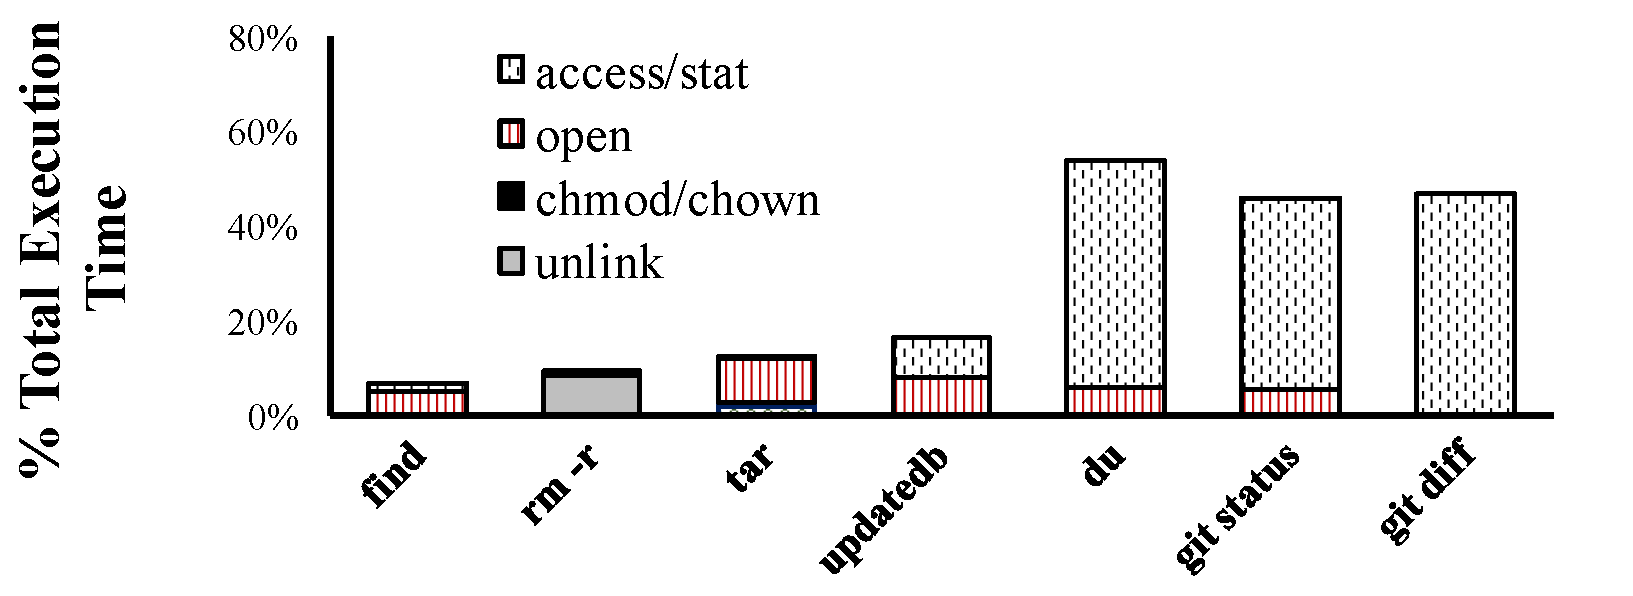
\includegraphics[width=5in]{dcache/plots/syscall-percentage.pdf} \\
\caption[Fraction of execution time on path-based system calls.]
{Fraction of execution time in several common utilities spent
executing path-based system calls with a warm cache, as measured with ftrace.}
\label{fig:dcache:lookup-frac}
%\vspace{-10pt}
\end{figure}

%\fixmedp{Please check these \% against time.  I think git diff is too high.  git status seems ok.}

Directory caches are essential for good application performance.
%Unix was designed such that ``(almost) everything is a file'',
%thus even accesses to in-memory file systems, device files, FIFOs and domain sockets
%first pass through the directory cache.
%In other words, 
Many common system calls must operate on file paths,
which require a directory cache lookup.
For instance, between 10--20\% of all system calls in the iBench system call traces do a path lookup~\citep{filenotafile}. 
Figure~\ref{fig:dcache:lookup-frac} lists the fraction of total execution time
%, as well as system time, 
several common command-line applications spend executing path-based system calls
(more details on these applications and the test machine in \S\ref{sec:dcache:eval}).
We note that these system calls include work other than path lookup,
and that these numbers include some instrumentation overhead;
% are coarse measurements that include  and work than path lookup;
%, and includes some time 
%for synchronous I/O (e.g., during {\tt rename}) as well as non-path tasks (e.g., creating 
%a file handle as part of {\tt open});
nonetheless, in all cases except {\tt rm},
the system call times and counts are dominated by
{\tt stat} and {\tt open}, for which 
%can be serviced from cache and for which 
path lookup is a significant component of execution time.
For these applications, path-based system calls account for 6--54\% of total execution time.
%and 25--77\% of system time.  
This implies that
lowering path lookup latency is
 one of the  biggest 
opportunities for a kernel to improve these applications' execution time.




\begin{figure}[t!]
\centering
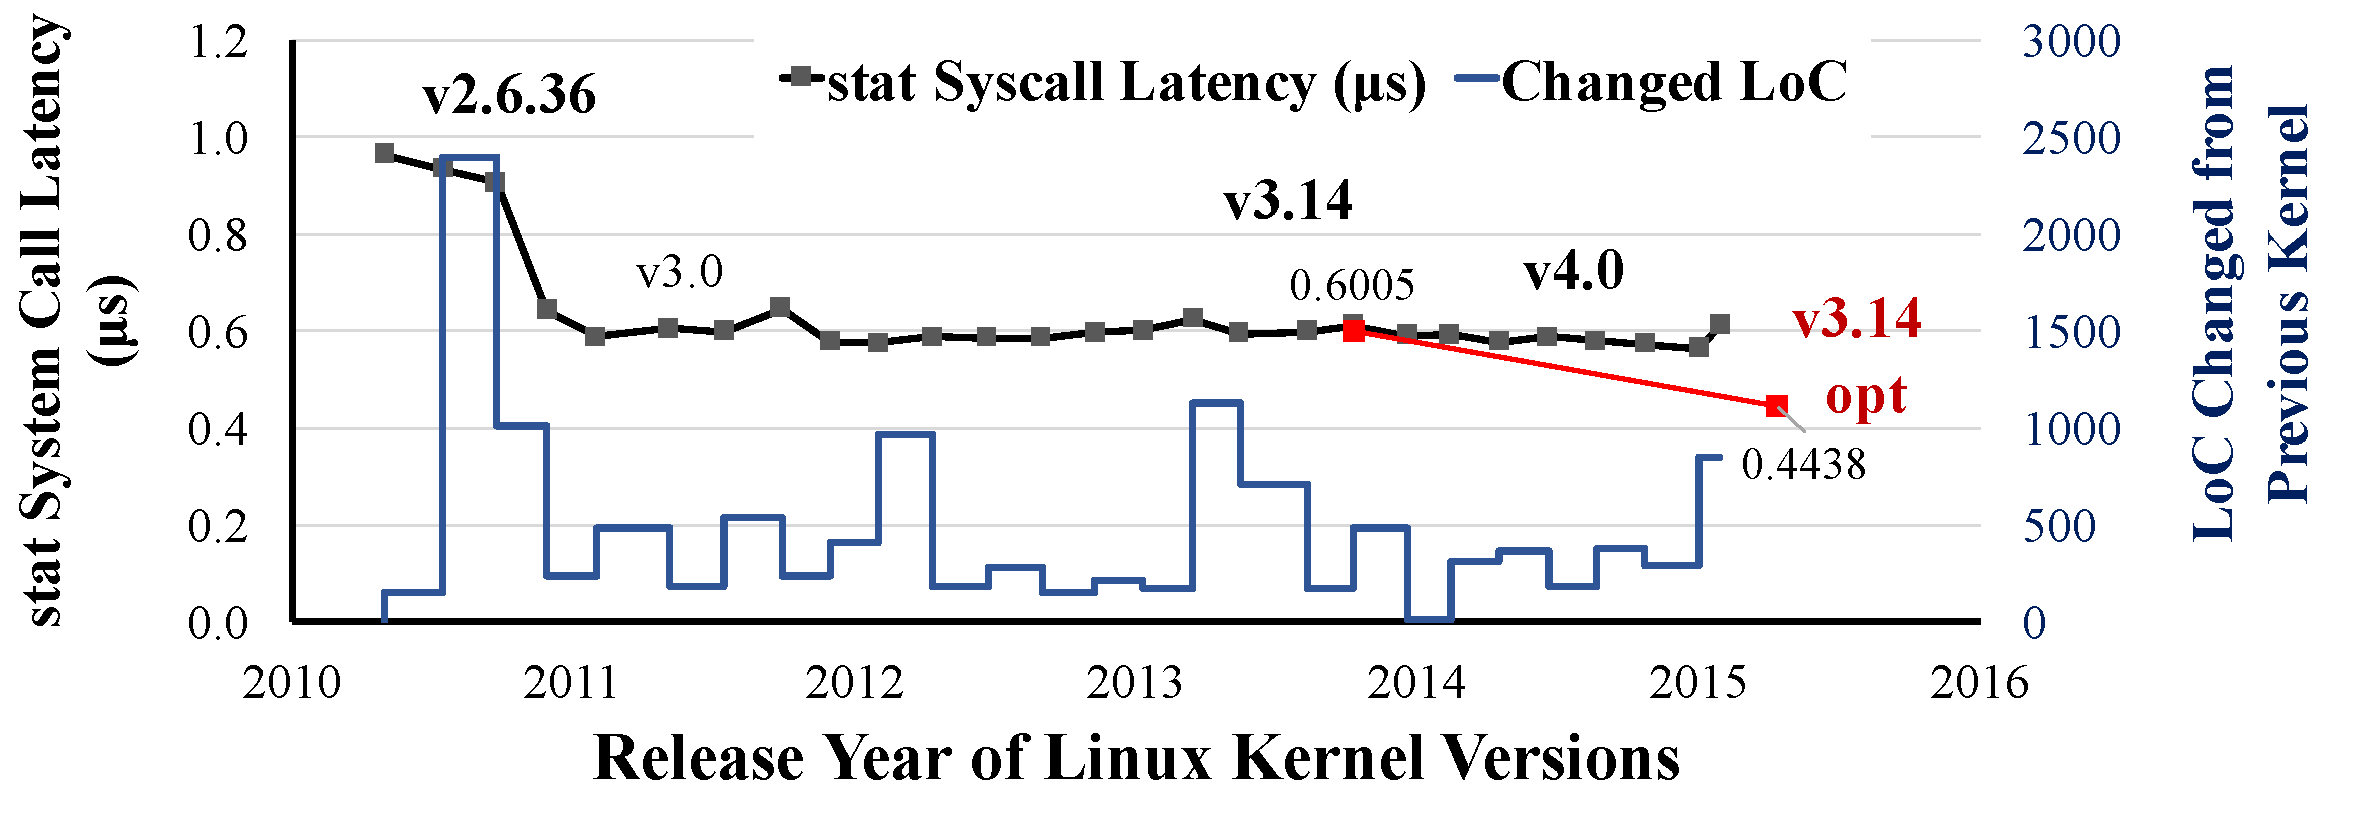
\includegraphics[width=6in]{dcache/plots/latency-by-version.pdf}
\footnotesize
\caption[Lantecy of {\tt stat} system call over years.]
{Latency of {\tt stat} system call with a long path {\tt XXX/YYY/ZZZ/AAA/BBB/CCC/DDD/FFF} on Linux over four years (lower is better), as well as the churn within the directory cache code (all insertions in {\tt dcache.c}, {\tt dcache.h}, {\tt namei.c}, {\tt namei.h} and {\tt namespace.c}). 
%Our optimizations significantly improve performance that has otherwise plateaued, despite significant ongoing developer effort.  
Our optimized \linuxver{} kernel 
further reduces {\tt stat} system call latency by \statspeedup{}\%.}
%\vspace{-15pt}
\label{fig:dcache:by-version}
\end{figure}


%\fixmedp{Add more evidence of lookup importance here: For instance, fraction of lookup time in file-related syscalls, or total lookup time in applications bound on file lookup latency.  }
Unfortunately, even directory cache hits are costly---0.3--1.1 \us{} for a {\tt stat} on our test Linux system, compared to only .04 $\mu$s for a {\tt getppid} and 0.3 \us{} for a 4 KB {\tt pread}. 
%\fixmetsai{Don, check this, I think read will be a better example, getppid is too trivial.}
This issue is taken particularly seriously in the Linux kernel community, which has 
made substantial revisions and increasingly elaborate optimizations to reduce the hit cost
of its directory cache, such as removing locks from the read path or replacing lock ordering with deadlock avoidance in a retry loop~\citep{corbet09jls,dcache-rcu}.
Figure~\ref{fig:dcache:by-version} plots directory cache hit latency against  lines of directory cache code changed 
over several versions of Linux, using a path-to-inode lookup \microbench{} on the test system described
in \S~\ref{sec:dcache:eval}.
These efforts have improved hit latency by 47\% from 2011 to 2013, but have plateaued
for the last three years.
%\fixmedp{if time, filter irrelevant changes from code deltas}
%at the cost of substantial developer effort.
%This latency appears to have plateaued 

The root of the problem is that the POSIX path permission semantics
seemingly require work that is linear in the number of path components,
and severely limit the kernel developer's implementation options.
%The root of this problem is that current directory cache
%designs reflect a straightforward implementation of the POSIX specification,
%which would seemingly require work that is linear in the number of path components.
For instance, in order to open file {\tt /\fnone{}/\fntwo{}/\fnthree{}} 
%for reading, 
one must have search permission
to parent directories {\tt /}, {\tt /\fnone{}}, and {\tt /\fnone{}/\fntwo{}},
as well as permission to access file {\tt \fnthree{}}.
The Linux implementation %of this specification is straightforward, 
simply walks the directory
tree top-down to check permissions.  
Unfortunately, when the critical path is dominated by 
walking a pointer-based data structure, 
including memory barriers on some architectures for multi-core consistency, 
modern CPUs end up stalling on hard-to-prefetch loads.
Moreover, because so many Linux features are built around this behavior, such as Linux Security Modules (LSMs)~\citep{wright+lsm},
namespaces, and mount aliases, it is not clear that any data-structural enhancements
are possible without breaking backward-compatibility with other Linux kernel features.
A priori, it is not obvious that a faster lookup algorithm, such as a single hash table lookup, 
can meet these API specifications and kernel-internal requirements; to our knowledge,
no one has tried previously.

%This paper proposes a decomposition of the directory cache, which allows
%most lookup operations to execute with a single hash table lookup (\S\ref{sec:dcache:dcache}),
%as well as optimizations to reduce the miss rate based on information that is {\em already in the cache}, but not used effectively (\S\ref{sec:dcache:readdir}).
%Our design maintains compatibility (\S\ref{sec:dcache:generalize}) through 
%several essential insights, including 
%how to separate the indexing of paths from checking parent permissions,
%and how to effectively and safely memoize the results of access control checks.


%% This paper proposes several new ways to organize a directory cache, which can yield 
%% substantial performance improvements over the current state of the art.
%% %This paper demonstrates that, despite this developer effort, there is still a substantial 
%% %missed opportunity hiding behind historical, intuitive, but not fundamental design choices.
%% Most of the Linux directory cache design reflects a straightforward implementation of the POSIX 
%% specification. %, with a division of labor that is suitable for mainstream file systems.

%This paper presents an alternative directory cache organization, which 
%improves performance by separating logical tasks, such as separating path indexing from permission checking; yet the design is sufficient to retain compatibility with POSIX.
%In the case of path lookup, 
%this paper demonstrates how 
%a per-component tree walk can be replaced with a single hash table lookup (\S\ref{sec:dcache:dcache}).
% without violating POSIX compliance.

%Our optimizations improve the performance of frequent lookup operations, but 
%introduce several costs, described in \S\ref{sec:dcache:dcache} and measured in \S\ref{sec:dcache:eval},
%which  we believe are acceptable and a net improvement for applications.
%First, these optimizations slow down infrequent modifications to the directory hierarchy, such as {\tt rename}, {\tt chmod},
% and {\tt chown} of a directory. 
%However, these slower operations
%account for less than .01\% of the system calls in the iBench traces~\citep{filenotafile}.
%Second,  the memory overheads of the dcache are increased.
%%(45\% per \dentry{}, as well as some  in our prototype).
%%(\fixmedp{XX MB} in our tests).  
%Third, lookup has a 
%probability of error from signature collisions that can be adjusted to be negligible
%%($2^{-141}$ in our configuration), 
%and within acceptable thresholds widely used by data deduplication systems~\citep{Debnath:2010:CSU:1855840.1855856, Srinivasan:2012:ILI:2208461.2208485, Quinlan:2002:VNA:645371.651321, Zhu:2008:ADB:1364813.1364831}.
%%, as well as how to remove
%%all memory barriers from the lookup path (\S\ref{sec:dcache:update}).
%In the micro-benchmark of Figure~\ref{fig:dcache:by-version}, our directory cache 
%optimizations improve lookup latency by 
%%revisions improve latency of accessing a long path
%%by 
%\statspeedup{}\% over unmodified Linux.
%%Our design addresses other missed
%%opportunities, such as identifying new opportunities to reduce the miss rate
%%through caching directory completeness.
%%\fixmedp{Do we want to highlight LoC?  3K is more than anything in the graph} \fixmetsai{Probably just mention in the evaluation. It's a metric that we should provide, but it's not awfully interesting.}
%%The total lines of code changed are fewer than 3,000 out of \fixmedp{XX}.
%%\fixmedp{Can we get 
%%, yet changes fewer than 3,000 lines of code.

%% SOSP cut - kind of long-winded
\begin{comment}
This paper rethinks current Linux directory cache design choices in light of the following goals:
\begin{compactitem}
\item {\bf Minimize the cost of a cache hit.} (\S\ref{sec:dcache:dcache}).
This means maximizing the benefit of temporal locality for frequent operations,
while pushing extra work of consistency maintenance onto less frequent, already-expensive operations.
%such as handling cache miss or updating massive metadata,
%in order to improve very frequent operations.
\item {\bf Maintain legacy compatibility.} (\S\ref{sec:dcache:generalize}).  Unix path semantics are complex, required by applications, file systems, and security modules, frustrating otherwise straightforward optimizations.  However tempting it may be to redesign path behavior to facilitate caching, path operations must exhibit the same behavior, with lower latency.
\item {\bf Never miss the same request twice in quick succession.} (\S\ref{sec:dcache:readdir}).  A number of less-frequent operations, such as reading a directory or secure temporary file creation, always miss in the cache {\em even if enough information is in cache to satisfy the operation.}  
%Of course, infrequent accesses should still be subject to a cache replacement policy, such as LRU.
\end{compactitem}
%Although directory caches must implement more complex semantics than a hardware memory cache,
%these principles should seem familiar to the reader with a basic architecture background.
%sadly, the Linux directory cache design violates all three.
\end{comment}

%This paper introduces several techniques to improve the performance of a directory cache,
%This paper explains several practical directory cache optimizations,
This paper demonstrates that these techniques improve performance for applications that use the directory cache heavily,
and the harm is minimal to applications that do not benefit.
%and that the worst case \microbench{} is only 12\% slower within \fixmedp{XX}\% of unmodified Linux.
%Each optimization we describe improves performance in isolation, and all can be combined.
%These optimizations change very few lines of code, and are backward-compatible with 
%legacy applications.  
%These changes are encapsulated in the VFS---individual file systems do not have to change their code.
%This paper describes a  prototype of these improvements implemented in Linux \linuxver{}.
%\S~\ref{sec:dcache:background} explains that the directory cache structure of Mac OS X, FreeBSD, and Solaris 
%are sufficiently similar that these principles should generalize.
%we compare and contrast Linux's directory cache
%with Mac OS X, FreeBSD, and Solaris in \S\ref{sec:dcache:background}, and explain inline how each
%optimization could be generalized to these other OS kernels.





%% \item {\bf Modularization and stackability}:
%% Any changes or optimizations must be implemented as modules inside Linux's VFS,
%% and can be stacked on top of the original design or any future optimizations. 
%% \item {\bf Backward compatibility}:
%% Any changes or optimizations must maintain least requirement of modifying any
%% file systems.
%% \item {\bf Generalization to other OSes}: Any changes or optimizations must be portable to other OSes with reasonable effort and change of design.




%% \dcache{} is proven to be effective on improving storage performance.
%% Experiments shows that,
%% in a Linux 3.x kernel, a \dcache{} with a xxx\% hit rate can speed up
%% metadata lookup and fetching time by xxx times.
%% \fixmetsai{experiment result, Linux version, and fs specs here}
%% However, we observed that Linux maintainers have made
%% constant and non-trivial efforts to improve \dcache{} in the Linux kernel.
%% We studied all \dcache{}-related source files in the Linux kernel Git repository,
%% and discovered that maintainers have committed
%% on average xxx revisions per source files.

%% We tested metadata lookup time on primary \dcache{}-related revisions.
%% Most changes on \dcache{} system only create xxx\%-xxx\% speed-up
%% than their predecessor.
%% \fixmetsai{result and graph here}.
%% Moreover, improvement to \dcache{} is still work-in-progress
%% for Linux maintainers.
%% \fixmetsai{reference to threads for latest dcache discussions}. 
%% All the evidences show that,
%% despite of significant reduction of storage operations,
%% efficiency of \dcache{} system internally still remains as a concern.

%% We argue that the design of \dcache{} needs to be carefully re-examined,
%% to fundamentally identify any missed opportunities that
%% improve value of \dcache{}.
%% At a high level, most optimization works for \dcache{} are focused on
%% improving ``how to cache'',
%% but we want to also lay eyes on ``what to cache'',
%% to ensure any valuable information returned from file systems
%% be captured by \dcache{} system.

%The contributions of this paper are as follows:
%\begin{compactitem}
%\item A performance analysis of the costs of path lookup and the opportunities
%to improve cache hit latency.
%\item A directory cache design that improves path lookup latency with a combination of techniques, including:
%  \begin{compactitem}
%  \item Indexing the directory cache by full path, reducing average-case lookup from linear to constant in the number of path components.
%  \item A Prefix Check Cache (PCC) that separates permission checking from path caching.  The PCC memoizes permission checks, and is compatible with LSMs~\citep{wright+lsm}.
%  \item Reducing the cost of checking for hash bucket collisions with path signatures.
%  \end{compactitem}
%\item Identifying opportunities to leverage metadata the kernel already has to reduce miss rates, such as tracking whether a directory is completely in cache.
%\item Carefully addressing numerous, subtle edge cases that would frustrate rote application of these techniques, such as integration with symbolic links and Linux namespaces.
%\item A thorough evaluation of these optimizations.  For instance, our optimizations improve throughput
%of the Dovecot IMAP server by up to \dovecotspeedup\% and latency of 
%updatedb by up to \updatedbspeedup{}\%.
%%git version control system by up to 25\%.
%
%\end{compactitem}

\section{API compatibility metrics}
\label{sec:metric:definitions}

We started this study from a research perspective, in search of a better way to evaluate
the completeness of system prototypes with a Unix compatibility layer.
In general, compatibility is treated as a binary property
(e.g., bug-for-bug compatibility), which loses 
important information when evaluating a prototype that is almost certainly incomplete.
Papers often appeal to noisy indicators that the prototype probably covers all important use cases,
such as the number of total supported system or library calls, as well as the variety
of supported applications.


These metrics are easy to quantify, but problematic.
Simply put, not all APIs are equally important: some are indispensable (e.g., \syscall{read} and \syscall{write}),
whereas others are very rarely used (e.g., \syscall{preadv} and \syscall{delete\_module}).
A simple count of system calls is easily skewed by 
system calls that are variations on a theme (e.g., \syscall{setuid}, \syscall{seteuid}, and \syscall{setresuid}).
Moreover, some system calls, such as \syscall{ioctl},
export widely varying operations---some used by 
by {\em all} applications and many that are essentially never used (\S\ref{sec:study:opcodes}).
%We use the term {\em vectored system call} for calls, such as {\tt ioctl},
%which essentially export a nested system call table, selected by an opcode argument.
%by {\em any} applications in Ubuntu 
Thus, a system with ``partial support'' for \syscall{ioctl}
is just as likely to support all or none of the Linux applications distributed with Ubuntu.



%This paper considers system APIs (``APIs'') broadly:
%this includes system calls, as well as any other means by which OS kernel functionality is
%requested, such as a pseudo-file system ({\tt /proc}).
%This paper also considers
%libraries like libc, which are typically responsible for exporting an API, like POSIX,
%as well as the primary way application developers interact with the OS kernel.
%For applications, system libraries are also system APIs. Modern applications rarely use the kernel interfaces like system calls directly, but instead call library APIs as wrapper or translation layer of kernel interfaces. 
%For Linux platforms, \libc{}, or {\em Standard Library C}, is the most ubiquitously used system libraries, providing a large fraction of
%general-purpose APIs commonly used by every application.


%%%  for the rest of the paper) as channels upon which
%%% applications request system functionalities,
%%% based on the contract between users and OS developers.
%%% The basic form of APIs on UNIX platforms is the system call,
%%% but others exist.
%%% For example, other APIs can be used through accessing system pseudo files or devices,
%%% such as {\tt /proc} files,
%%% or even communicating with administrative services using specific protocols (not covered in this paper).
%%% Although a API can contain multiple channels ---
%%% for instance, {\tt stat} system call provides several file attributes, or a pseudo file can be either read or written ---
%%% we group the usage data by system call numbers, vectored system call operation codes, and file paths,
%%% as the basic granularities of our analysis.  



%and easy to miss important cases in single system calls with a wide variety of options, such as {\tt ioctl}.

One of the ways to understand the importance of a given interface
is to measure its impact on end-users.  
In other words, if a given interface were not supported, how many users would notice its absence?
Or, if a prototype added a given interface, how many more users would be able to use the system?
%% probably don't need this note to Bianca
%\note{Drop footnote here.}
%\footnote{This assumes that the prototype is well-supported by the developers, and the maintainers have reasonable
%  installation instructions, are responsive to bug reports, etc.  The issues around maturity and support
%  of research prototypes are orthogonal to the question of which APIs need to be present
%  in a proof-of-concept system.}
To answer these questions, we must consider both the 
difference in API usage
among applications,
and the popularity of applications among end-users.
We measure the former by analyzing application binaries,
and determine the latter from installation statistics collected
by Debian and Ubuntu~\citep{ubuntu-popularity,debian-popularity}.
An {\bf installation} is a single system installation, and can 
be a physical machine, a virtual machine, a partition in a multi-boot system,
or a chroot environment created by {\tt debootstrap}.
Our data is drawn from over 2.9 million installations
(2,745,304 Ubuntu and 187,795 Debian).
%\fixmedp{Add a summary about how big this data set is (i.e., millions of systems)}
%Although difficult to measure directly, we approximate this based on package installation statistics~\citep{ubuntu-popularity}.


%%% This paper borrows the notion of installations from the package installation statistics.
%%% An {\em installation} represents a set of software installed in a standalone environment
%%% using the provided Ubuntu or Debian package installer.
%%% An installation does not necessarily represent a physical machine;
%%% it can be a partition in a multi-boot system,
%%% a virtual machine,
%%% or even a subsystem installed by 

We introduce two new metrics: one for each API, and one for a whole system.
For each API, we measure how disruptive its absence
would be to applications and end users---a metric we call {\bf  \usagemetric{}}.
For a system, we compute a weighted percentage we call {\bf \compatmetric{}}. 
For simplicity, we define a {\bf system} as a set of implemented or translated APIs,
and assume an 
application will work on a target system if the application's API footprint is implemented on the system.
These metrics can be applied to all system APIs,
or a subset of APIs,
such as system calls 
or standard library functions.
%pseudo-file system interfaces ({\tt /proc}),
%device interfaces ({\tt /dev}), or standard library functions.
%These metrics , and is fully generalizable to other families of OS distributions.



This paper focuses on \osdist{}, as it is a well-managed Linux distribution with a wide array of 
supported software, which also collects
package installation statistics.
The default package installer on \osdist{} is \osinstaller{}.
A {\bf package} is the smallest granularity of installation, typically
matching a common library or application.
A package may include
multiple executables, libraries, and configuration files.
Packages also track dependencies, such as a package containing 
Python scripts depending on the Python interpreter.
%Note that a package may install multiple executables,
%but the granularity of a package
%typically matches a single application or a set of 
%common, supporting libraries.
%one or more application binaries, but installation statistics are only collected
%at package granularity.
\osdist{} installation statistics are collected at package granularity
and collect several types of statistics.
This study is based on
data of how many
Ubuntu or Debian installations
installed a given target package.
%Other installation statistics are ignored,
%because they do not provide complete information about users' actual choices of packages.}
%\byinst{} shows how many systems installed the package,
%and \byvote{} shows how many systems regularly use the package.
%We calculate our measurements based on both data, depending on
%whether one is interested in supporting
%{\it all} packages installed on a system, or prioritizing {\it important} packages.

%%% For a system, a package is the smallest unit of installation.
%%% %by the package installer.
%%% Each package is a set of files that will be placed into the
%%% file systems. %when the package is installed.
%%% Note that a package does not always include standalone executables.
%%% Other files that can be found in a package
%%% includes scripts, shared libraries, configuration files,
%%% or even kernel extensions (modules).
%%% For those packages that do not include executables,
%%% our study tracks their dependencies. %of those packages.
%%% For example, a package containing Python scripts will depend on
%%% the Python package.
%%% We mark both packages as compatible if Python itself is supported.



For each binary in a package---either as a standalone executable or shared 
library---we use static analysis to identify all possible APIs the binary could call,
or the {\bf API footprint}.
The APIs can be called from the binaries directly,
or indirectly through calling functions exported by other shared libraries.
A package's API footprint is the union of the API 
footprints of each of its standalone executables.
We weight the API footprint of each package by its installation frequency
to approximate the overall importance of each API.
%Based on installation statistics of the package, we approximate the transitive importance of the system calls in each binary's footprint.
Although our initial focus was on evaluating research,
our resulting metric and data analysis provide insights for
the larger community, such as trends in API usage.



% Bug-for-bug compatibility beyond our scope; techniques largely orthogonal to this study; we assume that, once a given system call (say write) is supported and works for a reasonable sample of applications, handling edge cases should be straightforward engineering.  That said, for system calls 

%%% Put current metric discussion here

%% Then a subsection on approach and assumptions



\begin{comment}
API compatibility is one of most important system properties, for maintaining the availability of the whole system and decoupling the development of the OS and every applications.
For an OS of the size of Linux or Microsoft Windows, millions of softwares and subsystems are implemented on top of the platform,
counting on the API contracted to provide its services.
If a system engineer decides to change the API,
an inevitable risk is to sweep and update every existing applications accordingly, which are designed and maintained by countless third parties in the world.

Then, why would a system engineer try to change the API of an OS?
The answer is related with the procedure of developing an OS.
When an OS prototype is built, developers have to rely on experiences and instincts to make educated guess about what to be the ideal API of the system.
As time goes by, the OS gains a larger user base, and receives feedbacks about how the API should really be designed.
As soon as a developer realizes that refining the API can effectively improve either efficiency, robustness, security or user-friendliness of the system,
the risk of losing compatibility {\em slightly} can be totally worthy.

Unfortunately, the reality is that system engineers are frighten by the cost of refining the API for being unable to know how compatibility can be effected.
Since there is no data set about the actual usage of the API among applications, they must assume any application developers can potentially depend on the API.
It often takes a very long time, says 6 years \fixmetsai{LSB took 6 years, reference?}, to confirm, announce, communicate or simply wait until the API is officially deprecated.

We argue that knowing the API usage is the first step of understanding and evaluating compatibility.
Instead of using a realistic metric, system engineers often express the affects on API compatibility by numbers of interfaces that are implemented or modified.
Evaluation by counting the interfaces is extremely inaccurate, because every part of the API have different importance among applications.
Some interfaces are simply more frequently used and thus more important than others; for example, the consequence of changing system call {\tt open}, which is used ubiquitously,  is not the same as changing others like {\tt msgget}.
\end{comment}


\begin{comment}
%Bhushan: - Begin here -
Knowing the values of system interfaces among users is the prerequisite of evaluating platform compatibility.
When OS developers test their systems, a common approach is to prepare numerous test cases that exercise individual system interfaces.
It is often a natural thing to do for OS developers to maintain a list of supported system interfaces,
for either development purpose or advertisement.
However, because system interfaces have different values for users, they cannot be equal while evaluating platform compatibility of the OS.
A frequently used system interface should be considered more important for compatibility than a rarely used one.
\end{comment}

\subsection{\Usagemetric{}}

System developers can benefit from an importance metric for APIs,
which can in turn guide optimization efforts, deprecation decisions,
and porting efforts.  
Reflecting the fact that users install and use different software packages,
%Because users install different software on different systems, 
we define
\usagemetric{} as the probability that
an API will be indispensable to 
 at least one application on a randomly selected 
installation.
We want a metric that decreases
as one identifies and removes instances
of a deprecated API,
and a metric that will remain high for an indispensable API, 
even if only one ubiquitous application uses the API.



%, the  of that API will decrease.
%Similarly, an \usagemetric{} near 100 percent indicates an API is indispensable,
%at least for one ubiquitous application.
%The unsupported API with the highest \usagemetric{} creates an upper bound on 
%the system's overall  \compatmetric{}.
%For instance, if a system is missing an API with an \usagemetric{} of 20\%,
%the \compatmetric{} will never be higher than 80\% (but could be significantly lower).


%%% Given a complete list of installed applications in an OS installation,
%%% by examining the API footprint of every application,
%%% we can easily determine whether removing an API is disruptive for such an installation.
%%% %The result is a binary property: whether the API is important to
%%% %the installation or not.
%%% However, it is hard to predict what applications an installation will include.
%%% Thus, we define the metric for API usage as the probability
%%% that that target API
%%% is indispensable for an random installation.

%\vspace{0.1in}
%{\noindent
%\fbox{\begin{minipage}{\linewidth}
%\setlength{\parindent}{-0.1in}
%\setlength{\leftskip}{0.1in}
%\setlength{\rightskip}{0.1in}
% Definition: {\bf \UsageMetric{}.} \\
%For a given API, the probability that an installation includes
%at least one application requiring the given API.
%at least one broken application
%(whose API footprint covers the target API),
%if the target API was removed.
%\end{minipage}}}
%\vspace{0.1in}

\noindent Intuitively, if an API is used by no packages or installations,
the \usagemetric{} will be {\em zero}, causing no negative effects if removed.
We assume all packages installed in an OS installation are indispensable.
As long as an API is used by at least one package,
the API is considered {\it important} for the installation.
Appendix \ref{sec:defs:usagemetric} includes a formal definition of \usagemetric{}.
 
%% Besides the metric, the popularity of system interfaces can be important development hints as well.
%% Knowing the most and least valuable system interfaces of an OS,
%% the developers can make better decision on prioritizing the maintenance or retirement of the interfaces.
%% More influences of system interface popularity are discussed in \fixmetsai{later section?}.

%We define the popularity of a system interface by the probability that an installation become unsupported if the interface is removed.
%In other word, the popularity indicates the {\em cost} or {\em penalty} of deprecating an interface.

\begin{comment}
\paragraph{Formal Definition.}
A given system installation ($\mathtt{Inst}$)
is a set of packages installed ($\{\mathtt{pkg}_1, \mathtt{pkg}_2, ..., \mathtt{pkg}_k \in \mathtt{Pkg}_\mathtt{all}\}$).
For each package $\mathtt{pkg}$ in the \osdist{} repository,
our framework generates the API footprint as 
${\mathtt{Footprint}}_\mathtt{pkg} = \{\mathtt{api}_1, \mathtt{api}_2, ..., \mathtt{api}_k \in \mathtt{API}_\mathtt{all}\}$.  
For an API supported by the OS, we calculate the \usagemetric{} as the product 
of probabilities that an installed package will require this API.
This is calculated as follows:
\begin{align*}
&\mathtt{Dependent}_\mathtt{api} = \{\mathtt{pkg}|\mathtt{api} \in \mathtt{Footprint}_\mathtt{pkg}\} \\
&\mathtt{Importance}(\mathtt{api}) = Pr\{\mathtt{Dependent}_\mathtt{api} \bigcap \mathtt{Inst} \neq \emptyset\} \\
&= 1 - Pr\{\forall \mathtt{pkg} \in \mathtt{Dependent}_\mathtt{api}, \mathtt{pkg} \notin \mathtt{Inst}\} \\
&= 1 - \prod_{\mathtt{pkg} \in \mathtt{Dependent}_\mathtt{api}} Pr\{\mathtt{pkg} \notin \mathtt{Inst}\} \\
&= 1 - \prod_{\mathtt{pkg} \in \mathtt{Dependent}_\mathtt{api}} (1 - \frac{\text{installation of $\mathtt{pkg}$}}{\text{total installation}})
\end{align*}
\end{comment}


\subsection{\Compatmetric{}}

We also measure compatibility at the granularity of an OS,
which we call \compatmetric{}.
\Compatmetric{} is the fraction of applications that are likely to work,
weighted by the likelihood that these applications will be installed on a system.
%\fixmedp{check this synopsis}
% function of the APIs supported, weighted by the popularity 
%of the applications that require these APIs.

The goal of \compatmetric{} is to measure the degree to which a
new OS prototype or translation layer is compatible with a baseline OS.
In this study, the baseline OS is \osdist{}.



%%  as a function of the API footprint of each potentially-installed
%% application, weighted by the popularity of each application.
%% We introduce the metric , which we define in terms of an OS installation (i.e.,
%% the libraries and applications) and a target API implementation, which may provide a subset
%% of the original system's APIs.


%% An accurate metric for API compatibility must take into account at least two factors:
%% \begin{compactenum}
%% \item For each interface in the API, what are the applications that rely on it and could be affected if the interface is removed? ({\em application footprint})
%% \item For each application, how many installations of the system in the world has included it? ({\em application popularity})
%% \end{compactenum}


%% \fixmedp{Term for each call, vs system overall: API Importance and Effective Coverage?}

%% To accurately evaluate compatibility, we design a metric that is quantifiable, \fixmetsai{one more word here}, and easy to interpret.

\begin{comment}
We defined {\bf platform compatibility} as "{\em the probability of porting any installation of an OS distribution onto the target OS without any effort}".
The definition of an {\em installation} is a combination of application setup on a standalone OS instance.
An Installation can exist on physical machines,
or any machines of generalized sense such as a virtual machines, containers or subsystems.
In our model, installations represent customers of the OS, who are considered equal when providing any services.
\end{comment}

%\vspace{0.1in}
%\fixmetsai{Find a good name for our metric} 
%{\noindent
%\fbox{\begin{minipage}{\linewidth}
%\setlength{\parindent}{-0.1in}
%\setlength{\leftskip}{0.1in}
%\setlength{\rightskip}{0.1in}
%Definition: {\bf \CompatMetric{}.} \\
%For a target system, the fraction of applications supported,
%weighted by the popularity of these applications.
%For any installation, the expected fraction of installed applications that can work on the target OS.
%\fixmedp{shouldn't the weight go in the definition?}
%\Compatmetric{} is the total size of all supported applications,
%weighted by the popularity of each application.
%\end{minipage}}}
%\vspace{0.1in}

%\noindent In terms of porting effort, we are primarily interested in avoiding code changes, 
%such as {\tt \#ifdef LINUX}; although we leave this notion somewhat vague.
%We consider recompilation, relinking, or other mechanical processes acceptable.

%% Our analysis framework scans through all available packages in the \osdist{} repository and generates system interface footprint data for individual package.
%% The footprint data is based on static analysis,
%% and it lists all potentially used system interfaces regardless of the applications' runtime coverage. 
%% To build the metric, we also import the package popularity statistics from the official \osdist{} reports~\citep{ubuntu-popularity, debian-popularity}.

The methodology for measuring the \compatmetric{} of a target system's API subset is summarized as follows:
\begin{compactenum}
\item Start with a list of supported APIs of the target system, either identified from the system's source, or as provided by the developers of the system.
\item Based on the API footprints of packages, the framework generates a list of supported and unsupported packages.
\item The framework then considers the dependencies of packages. If a supported package depends on an unsupported package, both packages are marked as unsupported.
\item Finally, the framework weighs the list of supported packages based on package installation statistics.
As with \usagemetric{}, we measure the effected package that is most installed;
\compatmetric{} instead calculates the expected fraction of packages in a typical installation that will work on the target system.
%Specifically, each package's weight is based on 
%and the framework calculates the expected fraction of packages from a typical installation that will work on the target system.
\end{compactenum}
%\fixmedp{``typical installation'' raised some hackles.  Can we either use a different term, or talk more about this concept?}

\begin{comment}
\paragraph{Formal Definition.}
Suppose an OS supports a set of APIs ($\mathtt{API}_\mathtt{Supported}$),
% = \{i_1, i_2, ..., i_n\}$
which is a subset of the APIs of the original system ($\mathtt{API}_\mathtt{all}$).
In this study, $\mathtt{API}_\mathtt{all}$ is the sum of Linux APIs, including
the system call table, sysctl, proc, and so forth.
%(total APIs are $\Sigma = \{i_1, i_2, ..., i_m\}, m \geq n$).
A list of supported packages ($\mathtt{Pkg}_\mathtt{Supported}$) can be generated by checking whether the API footprint is
a subset of the target system's supported APIs ($\mathtt{API}_\mathtt{Supported}$):
\begin{align*}
\mathtt{Pkg}_\mathtt{Supported} = \{\mathtt{pkg} | \mathtt{Footprint}_\mathtt{pkg} \subseteq \mathtt{API}_\mathtt{Supported}\}
\end{align*}
\end{comment}


\vspace{10pt}
We note that this model of a typical installation is useful in reducing the metric to a single number,
but also does not capture the distribution of installations.
This limitation is the result of the available package installation statistics,
which do not include correlations among installed packages.
%Using package installation statistics has the important limitation that 
%which package installations are correlated.
This limitation requires us to 
assume that package installations are independent,
except when \osinstaller{} identifies a dependency.
For example, if packages {\em foo} and {\em bar} are both reported as being installed once,
we cannot tell if they were on the same installation, or if two different installations.
If foo and bar both use an obscure system API, we assume that two installations would be affected if the obscure API were removed.
If foo depends on bar, we assume the installations overlap. % overlapping installations are on the same system.
%We note that packages do include installation dependences, which could be used in future work to reduce this over-approximation.
%\fixmedp{Check my edit: I was confused by the old wording}
Appendix \ref{sec:defs:compatmetric} formally defines \compatmetric{}.



%% In our experiment, we assume installation of any packages to be {\em independent events}.
%% This is a strong assumption that can affect the precision of the metric.
%%  We introduce the assumption for the following reasons:
 
%%  \begin{compactenum}
%%  \item The official \osdist{} package popularity reports contain no relative popularity between packages. Neither is the raw data of individual installation published. 
%%  \item Most of the packages depend on others due to library dependency. Our analysis combines the popularity among libraries into the statistics of executables, and only counts executables for evaluation. 
%%  \end{compactenum}
 
%% As a limitation, we do not consider the case where executables may have relative popularity due to users' preference. For example, Apache-PHP-Mysql is a combination installed on many machines that provide web services.
%% In our experiment, we assume installation of each package is irrelevant with others.

\begin{comment}
Formally, \compatmetric{} is the expected fraction of packages on a given system($\mathtt{Inst}$)
having an API footprint within the target 
system's supported APIs.
%We approximate the expected value as follows:
%Based on the list of supported packages, we can calculate the probability of an installation $\zeta = \{p^{\zeta}_1, p^{\zeta}_1, ..., p^{\zeta}_q\}$ to be fully compatible as follows:
By assuming independence of package installation, we can calculate the probability of supporting an installation as follows:
\begin{align*}
&\mathtt{Weighted Compliance}(\mathtt{API}_\mathtt{Supported}) =\\
&E(\frac{|\mathtt{Pkg}_\mathtt{Supported} \bigcap \mathtt{Inst}|}{|\mathtt{Inst}|}) \sim \frac{E(|\mathtt{Pkg}_\mathtt{Supported} \bigcap \mathtt{Inst}|)}{E(|\mathtt{Inst}|)} \\
&\sim \frac{\sum_{\mathtt{pkg} \in \mathtt{Pkg}_\mathtt{Supported}} (\frac{\text{installation of $\mathtt{pkg}$}}{\text{total installation}})}{\sum_{\mathtt{pkg} \in \mathtt{Pkg}_\mathtt{all\hspace{0.21in}}} (\frac{\text{installation of $\mathtt{pkg}$}}{\text{total installation}})} \\
&\text{where E}(\mathtt{x})\text{ is the Expectation of }\mathtt{x}\text{ occurring.}
\end{align*}
\end{comment}

%% dp:Meh
%\subsection{Justifying the Practicability of the Metric}

\section{Data collection}
\label{sec:metric:collection}

We use static binary analysis to identify the system call footprint of a binary.  This approach has the advantages
of not requiring source code or test cases.  Dynamic system call logging using a tool like {\tt strace} is simpler,
but can miss input-dependent behavior.  A limitation of our static analysis is that we must assume the disassembled binary
matches the expected instruction stream at runtime.  In other words, we assume that the binary isn't deliberately obfuscating
itself, such as by jumping into the middle of an instruction (from the perspective of the disassembler).
%In practice, such obfuscation is generally done only by malware, and our results are not concerned with system security.
To mitigate this, we spot check that static analysis returns as superset of {\tt strace} results.

We note that, in our experience, things like the system call number or even operation codes are fairly straightforward
to identify from a binary.  These tend to be fixed scalars in the binary, whereas other arguments, such as the contents of a write buffer,
are input at runtime.
We assume that binaries can issue system calls directly with inline system call instructions, or can call system calls through a library, such as \libc{}.
Our static analysis identifies system call instructions and constructs a whole-program call graph.

\begin{figure}[t!]
\centering
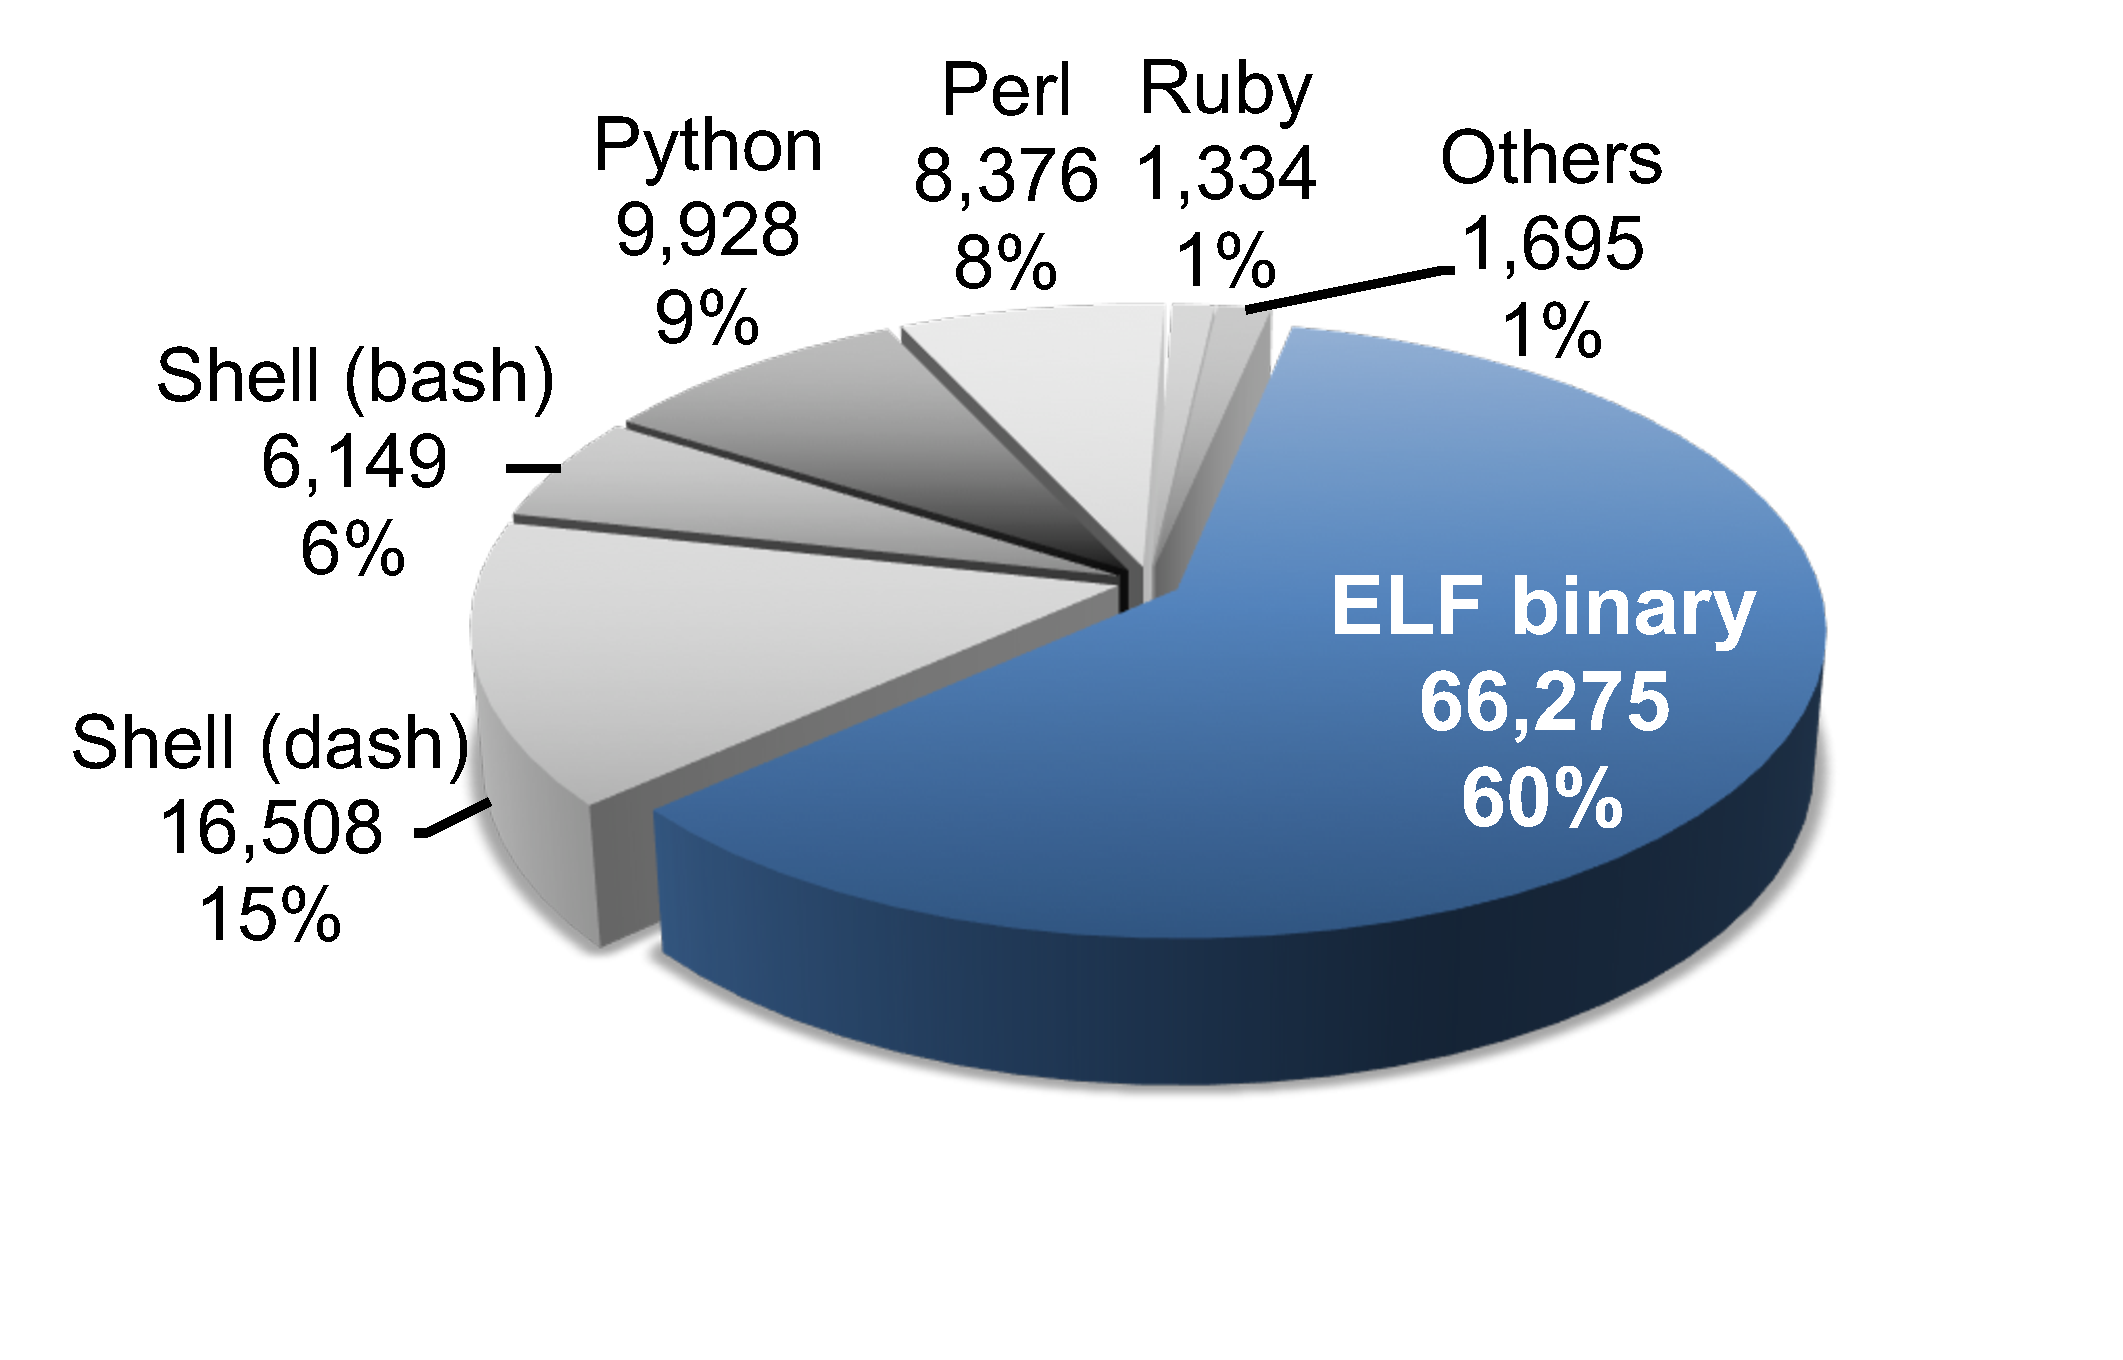
\includegraphics[width=3.2in]{executable-type.pdf}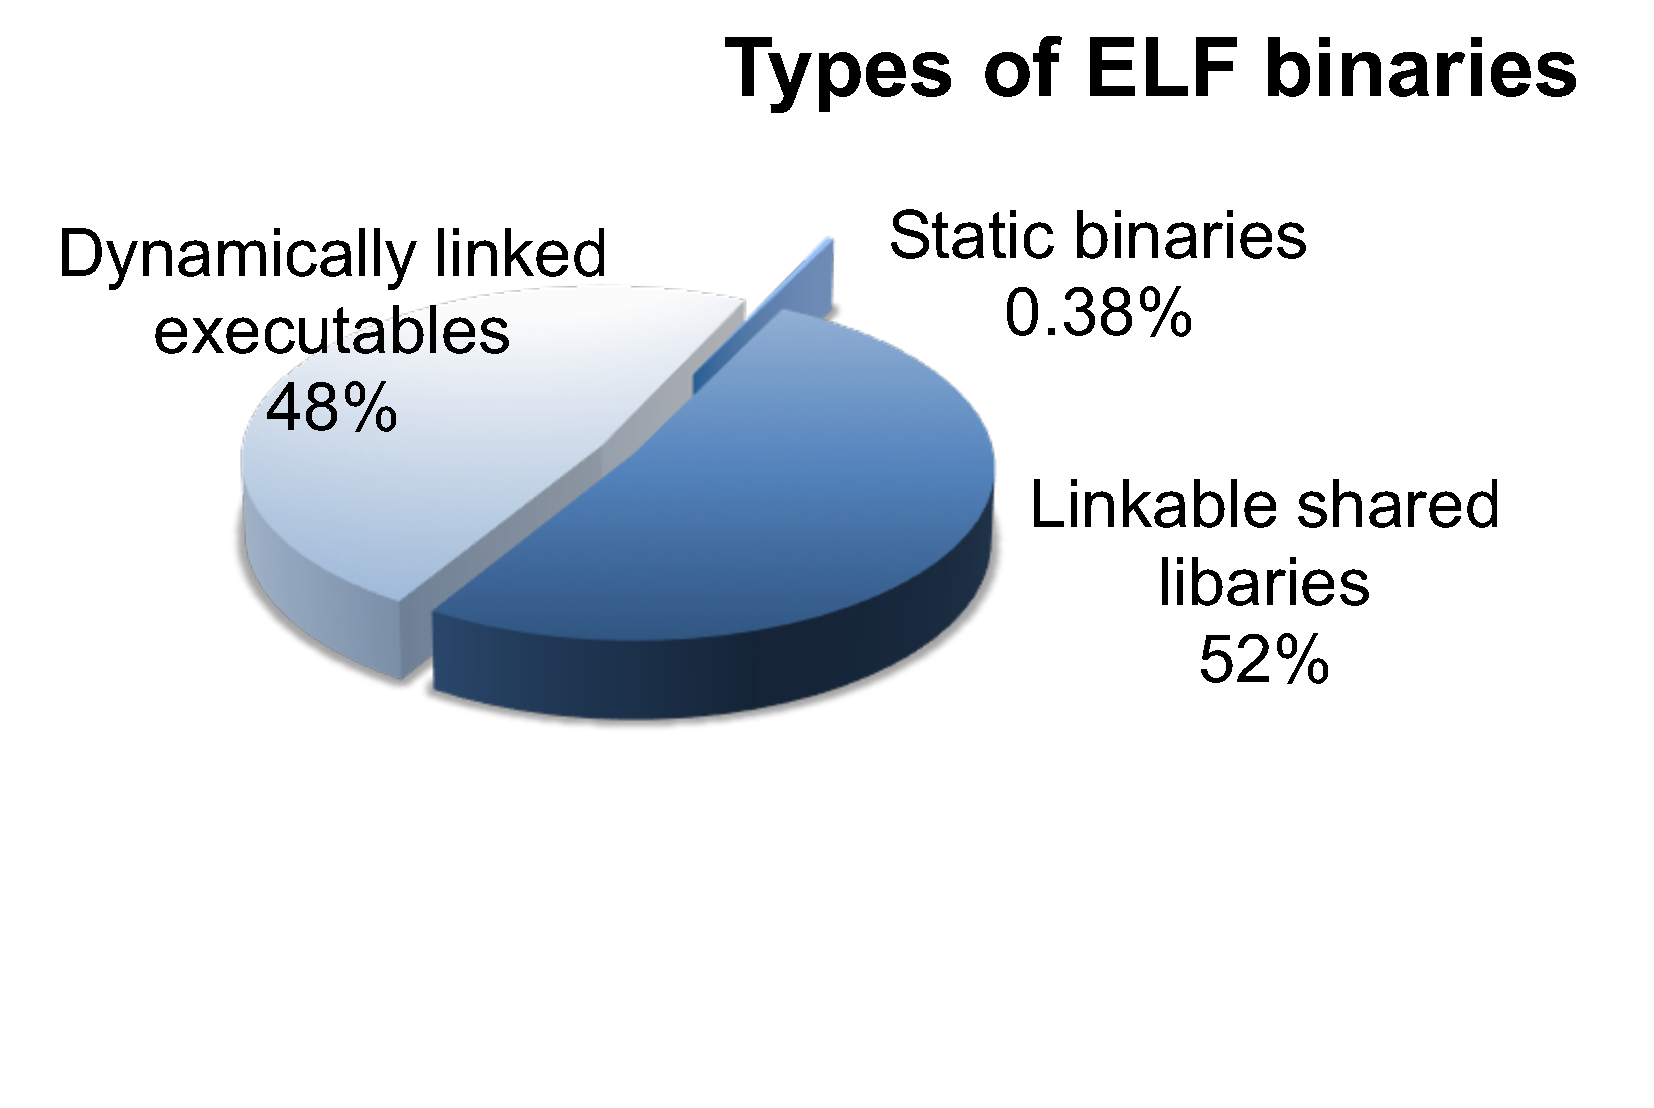
\includegraphics[width=2.4in]{elf-binary-type.pdf}
\vspace{-0.5in}
\footnotesize
\caption{Percentage of ELF binaries and applications written in interpreted languages among all executables in the \osdist{} repository, categorized by interpreters. ELF binaries include static binaries, shared libraries and dynamically-linked executables. Interpreters are detected by {\em shebangs} of the files. Higher is more important.}
\label{fig:syspop:executable-type}
\end{figure}

Our study focuses primarily on ELF binaries, which account for the largest fraction of Linux applications
%which account for the plurality of Linux applications
(Figure~\ref{fig:syspop:executable-type}).
For interpreted languages, such as Python or shell scripts,
we assume that the system call footprint of the interpreter and major supporting libraries over-approximates the expected system call footprint of the applications.
Libraries that are dynamically loaded, such as application modules or
language native interface (e.g.,JNI, Perl XS) are not considered in our study. 
%\fixmedp{Does the analysis handle JNI, Perl XS, or other wrappers for native libraries?  I 
%could imagine the answer being yes if a .so is shipped, but possibly no 
%if it is somehow inlined}

%\fixmedp{Maybe move this up and merge with discussion above}

%% Similarly, there is a distinction between installation and regular use.  Ideally, one might filter applications
%% that were installed but never used, or have a second variant of \usagemetric{} that is weighted by frequency of use.
%% %Although we leave this for future work
%% However, we hasten to note that some infrequently-used applications are nonetheless important to users,
%% and frequency-independent metrics are still important.
%Similarly, there is a distinction between installation and regular use.
%Figure~\ref{fig:package-popularity} shows the trend of package installation statistics for the 500 most commonly installed packages.
%The \byinst{} data may {\it over-approximate} the \usagemetric{} of a package,
%whereas the \byvote{} may {\it under-approximate} important, but infrequently used packages.
%We err on the side of over-approximating \usagemetric{}, using \byinst{}
%weighting where not otherwise specified,
%although we present measurements based on both when appropriate.
%instead under-approximating is a safer strategy to quarantee the compatibility requirements to be fully deliverable.
%In this paper, we present measurements based on both \byinst{} and \byvote{} statisitcs to draw more observations.

%\begin{figure}[t!]
%\vspace{-0.1in}
%\center{
%\includegraphics[width=3.6in]{figures/package-popularity.pdf}
%}
%\footnotesize
%\vspace{-10pt}
%\caption{Package installation statisitics in \osdist{}, for 500 most installed packages managed by the repository. \byinst{} shows installations of packages. \byvote{} shows regularly used packages voted by installations. Higher is more popular.\fixmebj{Change the scale.}}
%\label{fig:package-popularity}
%\end{figure}


\section{Implementation Details}
\label{sec:syspop:framework}

This section provides additional implementation details of our analysis framework. % for mining the API footprint for ELF executables and libraries.

%Analyzing the footprint of an applications requires interpretation of its behavior. As discussed in section~\ref{sec:measure:analysis}, we choose to build our framework by using {\bf static analysis} technique instead of dynamic analysis. The reason is that static analysis can trace potential executions of the applications, regardless of the runtime coverage of the code.

Our analysis is based on disassembling binaries inside each application package, using the standard {\tt objdump} tool.
This approach eliminates the need for source or recompilation, and can handle closed-source binaries.
We implement a simple call-graph analysis to detect system calls reachable from the binary entry point ({\tt e\_entry} in ELF headers). 
%\fixmedp{You do actually parse the elf header for e\_entry, right?}
%In our study, we only count executables during measuring both \usagemetric{} and \compatmetric{}.
We search all binaries, including libraries, for system call instructions ({\tt int \$0x80}, {\tt syscall} or {\tt sysenter}) or calling the {\tt syscall} API of \libc{}.
We find that the majority of binaries --- either shared libraries or executables --- do not directly choose system calls, but 
rather use the GNU C library APIs.
Among 66,275 studied binaries, only 7,259 executables and 2,752 shared libraries issue system calls.

% system calls. Therefore, analyzing the libraries that an executable depends on is necessary for retrieving a complete set of API footprint.


%, to predict its runtime behaviors.
%The framework requires no scanning of the source code, or recompiling of the applications with additional debug symbols.
%Consider the size and complexity of Ubuntu repositories,
%static analysis of ELF binaries is certainly easier to automate, and is able to analyze the applications that are close-sourced.

%To trace the footprint of applications, it require {\em Call-Graph Analysis} to rip off potential control flows that can eventually lead to usage of system API.
%Challenges of analyzing call-graph is a known issues for researchers in many area such as security, robustness, etc.

Our call-graph analysis allows us to only select system calls that are actually used by the application, not all the system calls that appear in \libc{}.
Our analysis takes the following steps:
\begin{compactitem}
\item For a target executable or a library, generate a call graph of internal function usage.
\item For each library function that the executable relies on, identify the code in the library that is reachable from each entry point called by the executable.
%trace coverage of code in the binary, and generate the minimal subset of the library's footprint that the function could actually link to.
\item For each library function that calls another library call, recursively trace the call graph and aggregate the results. 
\end{compactitem}
\vspace{10pt}

Precisely determining all possible call-graphs from static analysis is challenging.
Unlike other tools built on 
call-graphs, such as control flow integrity (CFI), our framework can tolerate the error caused by over-approximating the analysis results.
For instance, 
programs sometimes make function call based on a function pointer passed as an argument by the caller of the function. 
Because the calling target is dynamic, it is difficult to determine at the  call site.
Rather, we track sites where the function pointers are assigned to a register, such as using the {\tt lea} instruction with an address
relative to the current program counter.
%Instead of precisely tracking calling target at the {\tt call} instruction, 
%A function pointer is mostly assigned by {\tt lea} instruction to generate a relative address to the current program counter. 
This is an over-approximation because, rather than trace the data flow, we assuming that a function pointer assigned to a local variable will be called.
This analysis could be more precise if it included a data flow component. 
%\fixmedp{As an aside, this level of data flow analysis shouldn't be that hard, right?  Not  that it matters, except for the thesis/journal version.}

We also hard-code for a few common and problematic patterns.
For instance, we generally assume that the registers that pass a system call number to a system call,
or an opcode to a vectored system call, are not the result of arithmetic in the same function.
We spot checked this assumption, but did not do the data flow analysis to detect this case.

%must trace the register values such as {\tt RAX/EAX} for system call number or {\tt RBX/EBX} for parameter to vectored system calls. 

%Based on {\em Case-by-case study}, we assume no arithmetic but direct assignment of integers is possible when the program is issuing a system call. 

%If our analysis cannot precisely determine whether an API is used, we 
%err on the side of assuming an API is used.

%In the case of a run

%allow slightly enlarge the traced footprint of application, to gain simplicity for complex call-graph analysis corner cases. 
%For the specific run-time scenario of the application that can hard to interpret, we do a {\bf Case-by-Case study} to find out strategy of analyze the footprint practicably.

%  that call-graph analysis is complex for generating the accurate control flow of the run time. Fortunately, unlike other studies that relies on 

%In our study, we specifically call it {\bf Over-approximation}. 


%The following is a few example of using {\bf Over-approximation} and {\bf Case-by-Case study} to simplify call-graph analysis:
%\begin{compactenum}
%\item 
%\item 
%\end{compactenum}

Finally, the last mile of the analysis is to recursively aggregate footprint data. We insert all raw data into a {\tt Postgresql} database, and 
use recursive SQL queries to generate the results. 
To scan through all \packagenum{} packages in the repository, collect the data, and generate the results takes roughly three days.

   




\chapter{Evaluation}
\label{chap:eval}

\subsection{Limitations}
\label{sec:metric:limitations}

%\fixmedp{Make sure we explain these:  the fact that the new metrics cannot distinguish between APIs that are critical to a small population, in that their functionality cannot be provided any other way, because they are new APIs not yet widely adopted, or because they are old APIs that are no longer used or were never used.}

\paragraph{Popularity Contest Dataset.}
The analysis in this paper is limited
by the \osdist{}'s package installer, \osinstaller{},
and their package installation statistics.
Because most packages in \osdist{} are open-source,
our observations on Linux API usage may have a bias toward open-source development patterns.
Commercial applications that are purchased and distributed
through other means are not included in this survey data,
although data from other sources could, in principle, be incorporated
into the analysis if additional data were available.
%the analysis can only be conducted manually,
%thus making it really hard to collect large amounts of samples.

We assume that the package installation statistics provided by \osdist{} are representative.
%The \osdist{} repository hosts \packagenum{} packages that contain application executables and libaries. 
The popularity contest dataset is reasonably large (\popsamples{} installations),
but reporting is opt-in.
Moreover,
%\fixmedp{check this para}
%The popularity contest dataset does not correlate 
%package installations, only shows how often each package is installed.
%Thus, we assume the installation of every package
%as an independent event, unless \osinstaller{} identifies the dependency otherwise.
the data does not show how often these packages
are actually used, only how often they are installed.
Finally, this data set does not include sufficient historical data
to compare changes to the API usage over time.


%% Another limitation of using
%% the package installation statistics
%% is that the statistics only show
%% the installation count of each package,
%% but no details about which packages each installation contains or
%% relative preferences among packages.
%% Therefore, our study must 




%% dp: This is covered elsehwere
%The usage statistics collected in this paper generate
%convincing observations and measurements for Linux-compatible platforms,
%due to the large-scale analysis of software packages in the \osdist{} repository.
%Although our analysis does not require source code,
%our resulting dataset is mostly focused on open-source applications.
%Only very few applications in the \osdist{} repositories are close-source,
%such as the Nvidia driver utilities.
%Our analysis only requires application binaries, and our resulting dataset covers 
%both open-source and closed-source applications. \fixmedp{Right?  Double check that do include some closed binaries}
%Because we focus on \osdist{} applications, and most are open-source (xx\% \fixmetsai{Need to find this number, it's not hard.}),
%the data may be biased toward open-source applications. 
%As a result, our observations on Linux API usage are largely biased toward open-source applications.
%Because the repositories for close-source applications
%are more scattered
%(even though they can be downloaded by \osinstaller{} if manually configured),
%it is hard to collect large amount samples about them.

%% Our study is focused on applications managed by \osinstaller{},
%% which are mostly open-source
%% (even though our approach requires no source code for analysis).

\paragraph{Static Analysis.}
Because our study only analyzes pre-compiled binaries, some compile-time customizations may be missed.
Applications that are already ported using macro like {\tt \#ifdef LINUX} will be considered dependent to Linux-specific APIs,
even though the application can be re-compiled for other systems.
Our static analysis tool only identifies 
whether an API is potentially used,
not how frequently the API is used during the execution.
Thus, it is not sufficient to draw inferences about performance.

%This study is only sufficient to draw conclusions or insight about compatibility, not about any impact on performance.
%The static analysis on application binaries only tells
%Also the package installation statistics provide no information
%about how often a package is used.
%This study cannot provide evidence for whether any APIs may dominate
%execution time.


%\note{Move this here}
We assume that, once a given API (e.g., {\tt write}) is supported and works for a reasonable sample of applications,
handling missed edge cases should be straightforward engineering that is unlikely to invalidate the experimental results of the project.
That said, in cases where an input can yield significantly different behavior, e.g.,
the path given to {\tt open},
we measure the \usagemetric{} of these arguments.
Verifying bug-for-bug compatibility generally requires techniques largely orthogonal to the ones used in this study,
and thus this is beyond the scope of this work.

We do not do inter-procedural data-flow analysis.  As a result,
we were unable to identify system call numbers for 2,454 call sites (4\% of the
relevant call sites)
across all binaries in the repository.  As a result,
some system call usage values may be underestimated, and may go up 
with a more sophisticated static analysis.


%% The package installation statistics provided by \osdist{}
%% show only information about how often packages are ``installed'',
%% not how often packages are ``used''.
%% Our study is based on an over-approximation of the actual package usage:
%% installed packages in any installation contain
%% at least the packages actually used.


\paragraph{Metrics.}
The proposed metrics are intended to be simple numbers for easy comparison.
But this coarseness loses some nuance. 
For instance, our metrics cannot distinguish between
APIs that are critical to a small population, such as those that offer 
functionality that cannot be provided any other way, 
versus APIs that are rarely used because the software is unimportant.
Similarly, these metrics alone cannot differentiate a new API 
that is not yet widely adopted from an old API with declining usage.


%% Although studying historical data may provide more insight about
%% how developer or user behaviors change, our approach requires more historical data to make any conclusions.
%% The installation statistics contain no version information,
%% so it is insufficient to determine the adoption time of any application changes.
%% For packages, \osinstaller{} only keeps the latest version of each package in each maintained snapshot.
%% The only way to backtrace all historical versions of a package
%% is to pull from a version-control repository maintained by the package developers, which may not always exist.

\section{Implementation Details}
\label{sec:syspop:framework}

This section provides additional implementation details of our analysis framework. % for mining the API footprint for ELF executables and libraries.

%Analyzing the footprint of an applications requires interpretation of its behavior. As discussed in section~\ref{sec:measure:analysis}, we choose to build our framework by using {\bf static analysis} technique instead of dynamic analysis. The reason is that static analysis can trace potential executions of the applications, regardless of the runtime coverage of the code.

Our analysis is based on disassembling binaries inside each application package, using the standard {\tt objdump} tool.
This approach eliminates the need for source or recompilation, and can handle closed-source binaries.
We implement a simple call-graph analysis to detect system calls reachable from the binary entry point ({\tt e\_entry} in ELF headers). 
%\fixmedp{You do actually parse the elf header for e\_entry, right?}
%In our study, we only count executables during measuring both \usagemetric{} and \compatmetric{}.
We search all binaries, including libraries, for system call instructions ({\tt int \$0x80}, {\tt syscall} or {\tt sysenter}) or calling the {\tt syscall} API of \libc{}.
We find that the majority of binaries --- either shared libraries or executables --- do not directly choose system calls, but 
rather use the GNU C library APIs.
Among 66,275 studied binaries, only 7,259 executables and 2,752 shared libraries issue system calls.

% system calls. Therefore, analyzing the libraries that an executable depends on is necessary for retrieving a complete set of API footprint.


%, to predict its runtime behaviors.
%The framework requires no scanning of the source code, or recompiling of the applications with additional debug symbols.
%Consider the size and complexity of Ubuntu repositories,
%static analysis of ELF binaries is certainly easier to automate, and is able to analyze the applications that are close-sourced.

%To trace the footprint of applications, it require {\em Call-Graph Analysis} to rip off potential control flows that can eventually lead to usage of system API.
%Challenges of analyzing call-graph is a known issues for researchers in many area such as security, robustness, etc.

Our call-graph analysis allows us to only select system calls that are actually used by the application, not all the system calls that appear in \libc{}.
Our analysis takes the following steps:
\begin{compactitem}
\item For a target executable or a library, generate a call graph of internal function usage.
\item For each library function that the executable relies on, identify the code in the library that is reachable from each entry point called by the executable.
%trace coverage of code in the binary, and generate the minimal subset of the library's footprint that the function could actually link to.
\item For each library function that calls another library call, recursively trace the call graph and aggregate the results. 
\end{compactitem}
\vspace{10pt}

Precisely determining all possible call-graphs from static analysis is challenging.
Unlike other tools built on 
call-graphs, such as control flow integrity (CFI), our framework can tolerate the error caused by over-approximating the analysis results.
For instance, 
programs sometimes make function call based on a function pointer passed as an argument by the caller of the function. 
Because the calling target is dynamic, it is difficult to determine at the  call site.
Rather, we track sites where the function pointers are assigned to a register, such as using the {\tt lea} instruction with an address
relative to the current program counter.
%Instead of precisely tracking calling target at the {\tt call} instruction, 
%A function pointer is mostly assigned by {\tt lea} instruction to generate a relative address to the current program counter. 
This is an over-approximation because, rather than trace the data flow, we assuming that a function pointer assigned to a local variable will be called.
This analysis could be more precise if it included a data flow component. 
%\fixmedp{As an aside, this level of data flow analysis shouldn't be that hard, right?  Not  that it matters, except for the thesis/journal version.}

We also hard-code for a few common and problematic patterns.
For instance, we generally assume that the registers that pass a system call number to a system call,
or an opcode to a vectored system call, are not the result of arithmetic in the same function.
We spot checked this assumption, but did not do the data flow analysis to detect this case.

%must trace the register values such as {\tt RAX/EAX} for system call number or {\tt RBX/EBX} for parameter to vectored system calls. 

%Based on {\em Case-by-case study}, we assume no arithmetic but direct assignment of integers is possible when the program is issuing a system call. 

%If our analysis cannot precisely determine whether an API is used, we 
%err on the side of assuming an API is used.

%In the case of a run

%allow slightly enlarge the traced footprint of application, to gain simplicity for complex call-graph analysis corner cases. 
%For the specific run-time scenario of the application that can hard to interpret, we do a {\bf Case-by-Case study} to find out strategy of analyze the footprint practicably.

%  that call-graph analysis is complex for generating the accurate control flow of the run time. Fortunately, unlike other studies that relies on 

%In our study, we specifically call it {\bf Over-approximation}. 


%The following is a few example of using {\bf Over-approximation} and {\bf Case-by-Case study} to simplify call-graph analysis:
%\begin{compactenum}
%\item 
%\item 
%\end{compactenum}

Finally, the last mile of the analysis is to recursively aggregate footprint data. We insert all raw data into a {\tt Postgresql} database, and 
use recursive SQL queries to generate the results. 
To scan through all \packagenum{} packages in the repository, collect the data, and generate the results takes roughly three days.

   






\chapter{Linux API Study}
\label{chap:study}
\section{Linux API Study}
\label{sec:syspop:study}

%\note{about 3 pages, include graphs}
%\note{try to break the page here so the whole observation can start on a new page}

%This section presents measurements of API usage,
%as well as several trends in how APIs are used. Of particular note is that
%the OS interface required by essentially all applications is 
%%the total OS interface that essentially all applications require is
%substantially larger than the roughly 300 Linux system calls---the required interface
%also includes several vectored system call operations, such as {\tt ioctl}, and special filesystem interfaces like {\tt /sys} and {\tt /proc}.
%We also note that a number of system calls and other APIs are so rarely used that they can be deprecated with little disruption or effort.
%
%This section first examines the use of system calls in Linux applications.
%Section~\ref{sec:observation:hello} analyzes the most efficient path to add system calls
%to a prototype, outlining a path from the minimal footprint for ``hello world'', 
%up through the most demanding application (qemu), maximizing the number
%of supported applications at each step.
%Section~\ref{sec:observation:vector} analyzes the importance of operations
%under vectored system calls, such as {\tt ioctl}.
%Section~\ref{sec:observation:pseudo} evaluates the \usagemetric{} of 
%pseudo-files, such as those under {\tt /proc}.
%Finally, Section~\ref{sec:observation:libc}
%examines current usage patterns for \libc{}.
%Throughout the section, we identify several points at which APIs could be gainfully
%restricted, removed, or refactored,
%as well as identifying points where unexpected APIs can be essential to performance or
%functionality.
%We highlight key insights and recommendations in boxes.

%% \rev{Explain the structure.}{In the following subsections,
%% we will discuss our findings on the API usage of different interface types,
%% followed by %boxed take-aways our quick tips (in double-framed boxes)
%% the lessons or insights in boxes.} 
%% \fixmedp{If a reviewer asked for a structure, I expect they want to know something like:
%% We first present system calls, then ioctls,
%% then pseudo file systems, etc.  In other words, what is the organizing principle for 
%% the following sub-sections?  Not that we discuss and then have a box} 

%\subsection{\usagemetric{} of Linux System Calls}
\subsection{System calls}
\label{sec:syspop:study:syscall}

%We begin by looking at the \usagemetric{} of each system call, 
%ordered by total application installations and regularly used applications 
%in order to answer the following questions:
%\begin{compactitem}
%\item Which system calls are the most important to support when implementing a new system,
%or have high costs to replace, if desired?
%%1) do we definitely need to support any of the surveyed systems?
%%2) are used by at least one frequently used application on the surveyed systems?
%\item Which system calls are very rarely used and candidates for deprecation?
%\item Which system calls are not supported by the OS, but still attempted by applications?
%\end{compactitem}
%\vspace{10pt}

There are \syscallnum{} system calls defined in \osarch{} Linux \kernelversion{} (as listed in {\tt unistd.h}). 
Figure~\ref{fig:syscall-popularity-trend} shows the 
distribution of system calls by importance.
The Figure is ordered by most important (at 100\%) to least important (around 0\%)---similar
to inverted CDF.
The figure highlights several points of interest on this line.

%The trends \byinst{} are useful to answer questions about supporting complete installations, 
%while the trends \byvote{} are useful to answer questions about supporting most popular 
%applications on most of the systems.
Over two-thirds ({\em 224 of \syscallnum{}}) 
of system calls on Linux are indispensable:
required by 
at least one application on every installation.
%only a little 
%over one-thirds ({\em 121 of \syscallnum{}}) of system calls are required 
%by at least one regularly used application (\byvote{}).
%\fixmedp{Would be nice to have more to say here, like filling out weighted compliance and the number of packages}
Among the rest, 33 system calls are important on more than ten percent of the installations.
44 system calls have very low \usagemetric{}:
less than ten percent of the installations include at least one application
that uses these system calls.
%Moreover, less than 10\% of the systems require 43 system calls.
%and 58 system calls are regularly used on less than 10\% of the systems (\byvote{}).
%For instance, {\tt timer\_delete}, {\tt timer\_create} and {\tt timer\_settime} are used by 
%at least one application on all the systems, however, the applications using these 
%system calls are regularly used only on 17\% of the systems. 
%Another system call 
%{\tt tkill} used by {\tt strace} installed ubiquitously on all systems 
%is used regularly only on 3\% of the systems. So, even if the installation statistics imply that 
%{\tt tkill} needs to be supported to support at least one of the machines,
%only 3\% of those machines regularly use that system call.

Our study also shows the contributors
to an API's importance. %\usagemetric{}.
For instance, Table~\ref{tab:syspop:wrapped} lists system calls that are
only called by one or two particular libraries
(e.g., \libc{}).
These system calls are wrapped by library APIs,
so applications depend on them only because the libraries do.
To eliminate the usage of these system calls,
developers only have to pay minimum efforts to re-implement the wrappers in libraries.

\begin{figure}[t]
\centering
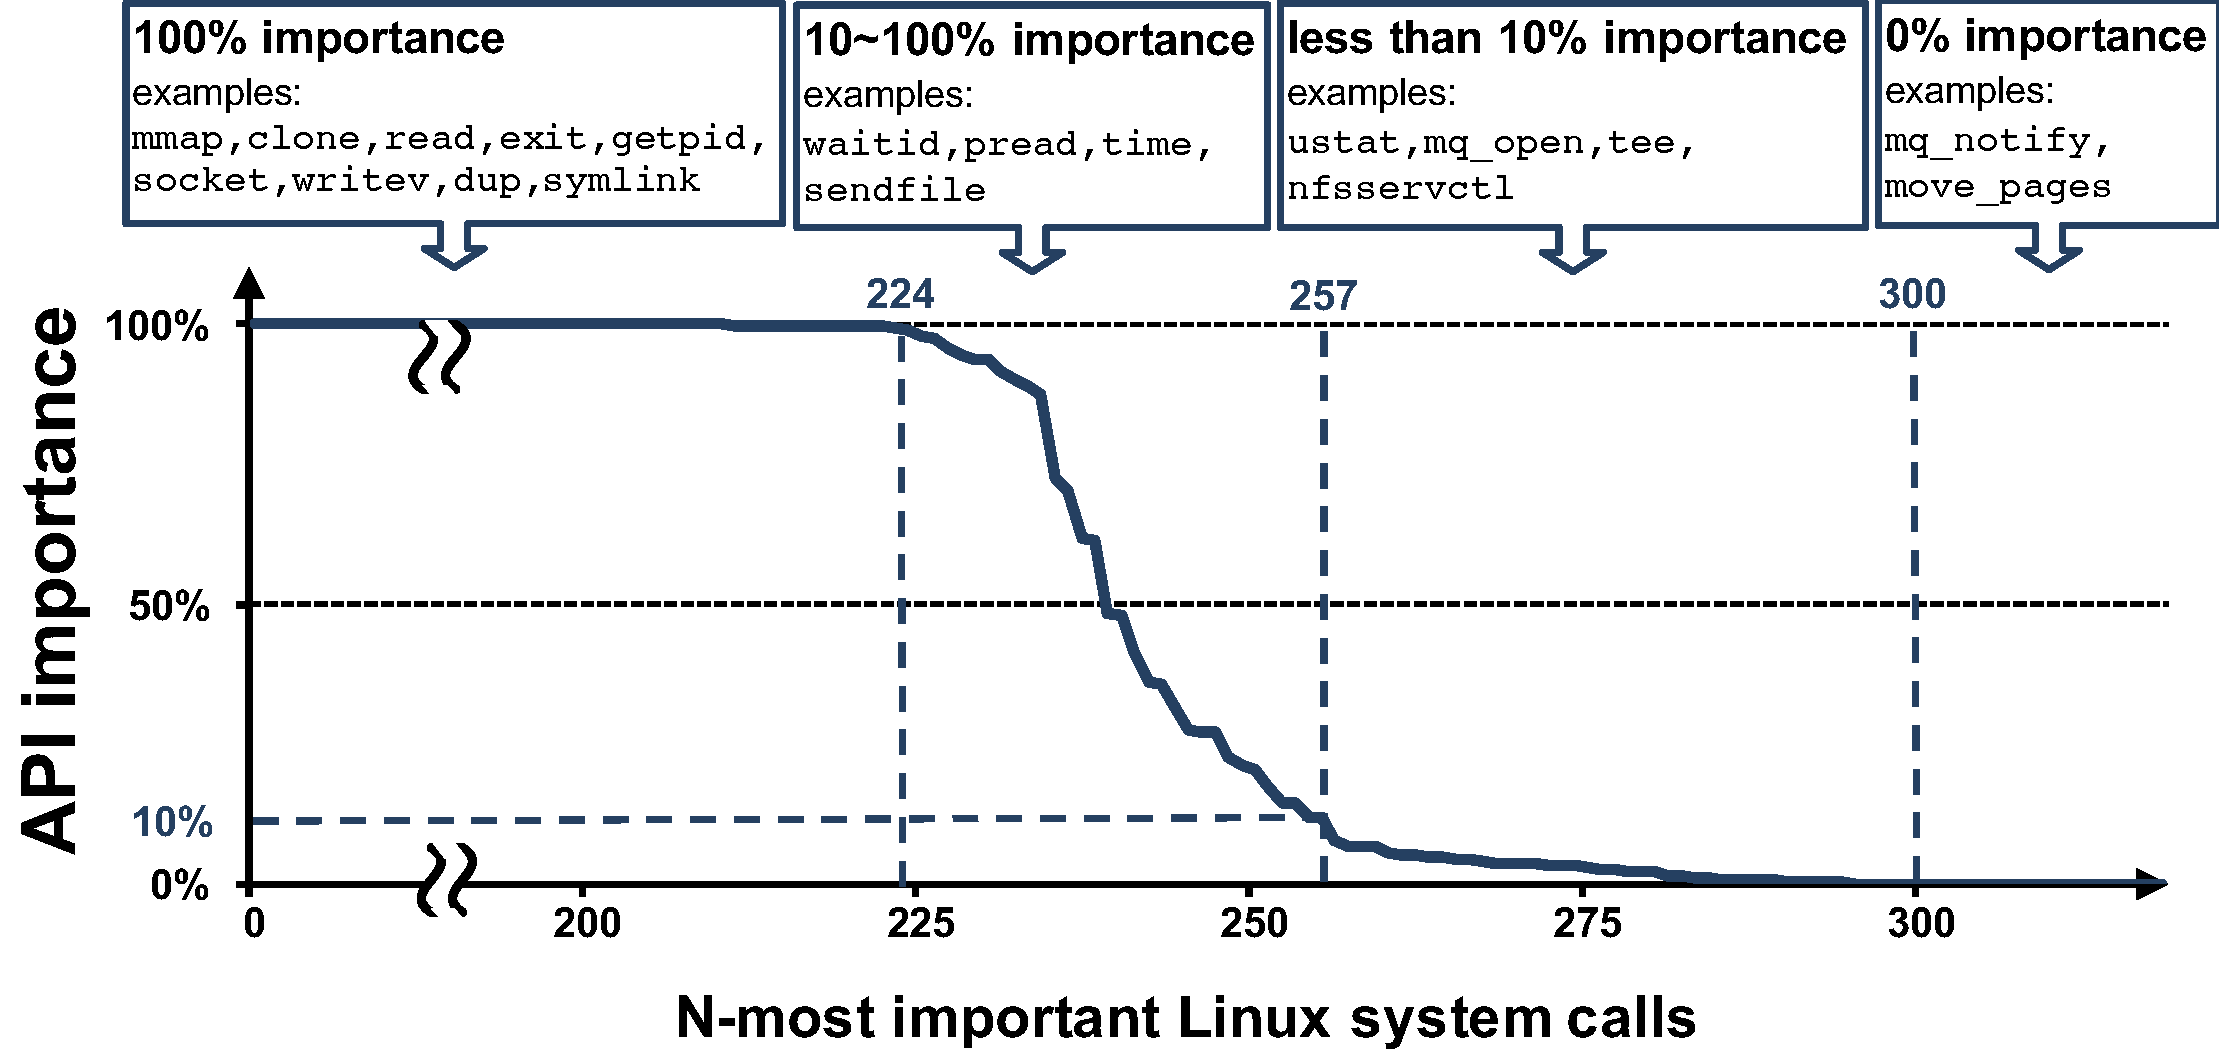
\includegraphics[width=\textwidth]{syscall-popularity-all-by-inst.pdf}
\caption[N-most important system calls in Linux.]
{The trend of \usagemetric{} as N-most important system calls among total \syscallnum{} system calls of \osversion{} with Linux kernel \kernelversion{}. .
Higher is more important; 100\% indicates all installations include software that make the system call.}
\label{fig:syscall-popularity-trend}
\end{figure}

%\callout{It is easy to support regularly used parts of an installation than complete installations of the surveyed systems.} 

Among the 44 system calls with a \usagemetric{} above zero but less than ten percent,
some are cases where a more popular alternative is available.
%developers appear more motivated by 
%portability than security.
%, the bottom 20 non-zero are listed in Table~\ref{tab:syscall-popularity-bottom}, along with the packages that use these interfaces.
%%11 of the bottom 20 system calls are Linux-specific.
%%This shows that portability to other Unix variants
%%has a significant effect on adoption.
%%bP: These conclusions cannot be made with weighted importance.
For instance, Linux supports both POSIX and System V message queues.
The five APIs for POSIX message queues have a lower
\usagemetric{} than System V message queues.
We believe this is attributable to System V message queues %provide a better designed interface, they
being more portable to other UNIX systems.
%they are not adopted by most popular applications.}
Similarly, we observed that {\tt epoll\_wait} (100\%) has a higher \usagemetric{} than {\tt epoll\_pwait} (3\%),
even though {\tt epoll\_pwait} is commonly considered more robust
for the same purpose---waiting on file descriptor events.
Table~\ref{tab:dominated} lists
system calls used by only one or two packages---generally special-purpose utilities,
such as {\tt kexec\_load}, which is used by {\tt kexec-tools}).
%,These system calls are mostly used by special-purpose utilities (e.g., 
%and generally address  because their semantics are not friendly enough.

\begin{table}[t!b!]
  \centering
  \small
  \begin{tabular}{>{\footnotesize\raggedright\arraybackslash}p{1.45in} >{\raggedleft\arraybackslash}p{0.25in}>{\raggedright\arraybackslash}p{1.15in}}
\toprule
{\bf System Calls} & {\bf Imp.} & {\bf Packages}\\
\midrule
{\tt clock\_settime}, {\tt iopl}, {\tt ioperm},  {\tt signalfd4}  & 100\% & libc \\
{\tt mbind}             & 36.0\% & libnuma, libopenblasp \\
{\tt addkey}            & 27.2\% & libkeyutils \\
{\tt keyctl}            & 27.2\% & pam\_keyutil, libkeyutils \\
{\tt requestkey}        & 14.4\% & libkeyutils \\
{\tt preadv}, {\tt pwritev}   & 11.7\% & libc \\
    \end{tabular}%
   \caption{System calls which are only directly used by particular libraries, and their \usagemetric{} (``Imp.''). Only system calls with \usagemetric{} larger than ten percent are shown.
These system calls are wrapped by library APIs,
thus they are easy to deprecate by modifying the libraries.  
}
  \label{tab:wrapped}%
\end{table}%

\begin{table}[t!b!]
\centering
\small
\begin{tabular}{>{\palign[\footnotesize]{l}}p{2.9in} >{\palign{r}}p{1.1in}>{\palign{l}}p{2in}}
\toprule
{\bf System Calls} & {\bf \UsageMetric{}} & {\bf Used Packages}\\
\midrule
{\tt seccomp}, {\tt sched\_setattr}, {\tt sched\_getattr}  & 1\% & coop-computing-tools \\
\hline
{\tt kexec\_load} & 1\% & kexec-tools \\
\hline
{\tt clock\_adjtime} & 4\% & systemd \\
\hline
{\tt renameat2} & 4\% & systemd, coop-computing-tools \\
\hline
{\tt mq\_timedsend}, {\tt mq\_getsetattr} & 1\% & qemu-user \\
\hline
{\tt io\_getevent} & 1\% & ioping, zfs-fuse \\
\hline
{\tt getcpu} & 4\% & valgrind, rt-tests \\
\hline
\end{tabular}%
\caption[System call usage dominated by particular package(s)]
{System calls with usage dominated by particular package(s), and their \usagemetric{}. This table excludes system calls that are officially retired.}
\label{tab:dominated}%
\end{table}%


In some cases, system calls are effectively offloaded to a file in {\tt /proc} or {\tt /sys}.
For instance, some of the information that was formerly available via 
{\tt query\_module} can be obtained from {\tt /proc/modules}, {\tt /proc/kallsyms} 
and the files under the directory {\tt /sys/module}. Similarly, the information that can be obtained from the {\tt sysfs} system call
is now available in {\tt /proc/filesystems}.

%We found five  API that have very low 
%compared to the System V message queue API.

We also found five system calls {\tt uselib}, {\tt nfsservctl}, {\tt afs\_syscall}, {\tt vserver} and {\tt security} system calls that are officially retired, but still have a low, but non-zero, \usagemetric{}. 
For instance {\tt nfsservctl} is removed from Linux kernel 3.1 but
still has \usagemetric{} of seven percent,  %\fixmedp{Do we have some examples of apps that use it?}
because it is tried by NFS utilities such as {\tt exportfs}.
These utilities still attempt the old calls for backward-compatibility with older kernels.
%Application maintainers of packages using these retired system calls need to be notified to port their applications to support latest kernel.


%\callout{System developers can use our framework to actively notify relevant package maintainers while retiring system calls.} 
%\callout{Among 43 least-used system calls, some are replaceable
%by alternatives with higher \usagemetric{};
%5 are officially retired but still tried by few applications.
%System developers could use this data to identify relevant applications,
%accelerating replacement of these system calls.}




\begin{table}[t!b!]
\centering
\small
\begin{tabular}{>{\palign[\footnotesize]{l}}p{.5\textwidth} >{\palign{l}}p{.45\textwidth}}
\toprule
\textbf{Unused System Calls} & \textbf{Reason for Disuse}\\
\midrule
{\footnotesize
{\tt set\_thread\_area}, {\tt tuxcall}, {\tt create\_module}, and 7 more. } & Officially retired.\\
\hline
{\tt sysfs} & replaced by {\tt /proc/filesystems}.\\
\hline
{\tt rt\_tgsigqueueinfo}, {\tt get\_robust\_list} & Unused by applications.\\
\hline
{\tt remap\_file\_pages} & No non-sequential ordered mapping; repeated calls to mmap preferred.\\
\hline
{\tt mq\_notify} & Unused: Asynchronous message delivery.\\
\hline
{\tt lookup\_dcookie} & Unused: for profiling.\\
\hline
{\tt restart\_syscall} & Transparent to applications.\\
\hline
{\tt move\_pages} & Unused: for NUMA usage. \\
\hline
\end{tabular}%
\caption{Unused system calls and explanation for disuse.}
\label{tab:syspop:unused}%
\end{table}%



%On the other end of the spectrum, 

In total, 18 of \syscallnum{} system calls in Linux \kernelversion{} are not used by any application in the \osdist{} repository. We list these system calls in Table~\ref{tab:syspop:unused}.
In addition to the issues discussed above,
Ten of these system calls do not have an entry point, but are still defined in the Linux headers.
%\fixmedp{Why are they in the count then?  do you mean 320 defined system call numbers}
%Similarly, we analyze the 21 system calls with 0 \usagemetric{} as shown in 
%Table~\ref{tab:unused}. 
%{\tt sysfs} is replaced by alternate interface {\tt /proc/file\linebreak[0]systems}.
%%On the other hand, even though {\tt remap\_file\_pages} system call was added to map pages of a file into memory in a non-sequential order since Linux version 2.6 (in 2003), no application is actually using it. This indicates that either no application is mapping pages in non-sequential order or applications are repeatedly using the more popular generic system call like {\tt mmap}.
%Similarly, {\tt mq\_notify} system call for receiving asynchronous notification about new messages in message queue is not used, because \usagemetric{} of message queue interfaces is less than 5\% in the first place and applications using message queue do not use asynchronous communication.
Five of the unused system calls such as {\tt rt\_tgsig\linebreak[0]queueinfo}, {\tt get\_robust\_list}, {\tt remap\_\linebreak[0]file\_pages}, {\tt mq\_notify}, {\tt lookup\_dcookie} provide an interface that is not used by the applications. These system calls can be potential candidates for deprecation.
However, even though {\tt restart\_\linebreak[0]syscall} is not used by any application, it is internally used by the kernel. % transparent to userspace.
%Finally, 4 NUMA related system calls are not used 
%\rev{rewrite}{because none of our samples is written to be NUMA-aware}.
%\fixmetsai{Check if libnuma uses these system calls.}

%\callout{In addition to ten already retired system calls, we found seven other candidate system calls for deprecation or in need of more exposure to developers.}

\begin{comment}
\begin{table}[t]
\center{
\footnotesize
\begin{tabular}{m{0.45\linewidth}m{0.45\linewidth}}
\hline
Syscalls & Packages\\
\hline
process\_vm\_writev & coop-computing-tools, care, proot, stress-ng \\
vserver & util-vserver\\
syncfs & ceph-test, ploop, ruby-passenger, ceph\\
io\_getevents & ioping, zfs-fuse\\
uselib & mupdf, mupdf-tools\\
afs\_syscall & openafs-fileserver, openafs-kpasswd, openafs-krb5, openafs-client, openafs-dbserver\\
kexec\_load & kexec-tools\\
mq\_getsetattr, mq\_timedsend & qemu-user, qemu-user-static\\
vmsplice & criu, qemu-user-static, fio, stress-ng, qemu-user\\
timer\_gettime & ben, galax-extra, libocamlnet-ocaml-bin, ocsigenserver, galax, approx, qemu-user-static, galaxd, matita, cduce, qemu-user, turnserver, stress-ng\\
timerfd\_gettime & ben, approx, libocamlnet-ocaml-bin, ocsigenserver, openclonk, matita, galax, galaxd, qemu-user-static, galax-extra, cduce, qemu-user\\
eventfd & blktap-utils, julia, nodejs\\
semtimedop & tgt, dahdi, gtk-gnutella, prayer, libopenni-sensor-primesense0, libopenni-sensor-pointclouds0\\
timer\_getoverrun & emacs24-lucid, emacs24, qemu-user-static, qemu-user, emacs24-nox, rt-tests, reconserver, miredo\\
mq\_timedreceive & qemu-user-static, nilfs-tools, xjadeo, rt-tests, qemu-user\\
acct & watchdog, acct, qemu-user-static, qemu-user, scm, atop\\
fanotify\_init, fanotify\_mark & fatrace, fnotifystat, health-check, clamav-daemon\\
open\_by\_handle\_at & qemu-system-mips, qemu-system-misc, qemu-system-sparc, qemu-system-ppc, qemu-system-arm, qemu-system-x86\\
\hline
\end{tabular}
}
\footnotesize
\caption{20 system calls with the lowest \usagemetric{} among 297 used system calls in \osversion{} with Linux Kernel \kernelversion{}, except the ones with \usagemetric{} lower than 0.01\% (considered negligible).}
\label{tab:syscall-popularity-bottom}
\end{table}
\end{comment}

\begin{comment}
There are 43 system calls with low non-zero \usagemetric{} of less than 10\%.
%, the bottom 20 non-zero are listed in Table~\ref{tab:syscall-popularity-bottom}, along with the packages that use these interfaces.
%%11 of the bottom 20 system calls are Linux-specific.
%%This shows that portability to other Unix variants
%%has a significant effect on adoption.
%%bP: These conclusions cannot be made with weighted importance.
We found 5 POSIX message queue API that have very low 
\usagemetric{} compared to the System V message queue API because 
even if POSIX message queues provide a better designed interface, they are less 
widely available. We also found 5 system calls {\tt uselib}, {\tt nfsservctl}, {\tt afs\_syscall}, {\tt vserver} and {\tt security} system calls that are officially retired, and have non-zero albeit negligible \usagemetric{}. 
For instance {\tt nfsservctl} is removed from Linux kernel 3.1 but
still has \usagemetric{} of 7\%. Application maintainers of packages using these retired system calls need to be notified to port their applications to support latest kernel.
Also, we observed that {\tt epoll\_wait} (100\%) has more \usagemetric{} than {\tt epoll\_pwait} (3\%)
even though {\tt epoll\_pwait} is safer to use to wait for a file descriptor to become available.
In some cases, system calls are effectively offloaded to a file in {\tt /proc} or {\tt /sys}.
For instance, some of the information that was formerly available via 
{\tt query\_module} can be obtained from {\tt /proc/modules}, {\tt /proc/kallsyms} 
and the files under the directory {\tt /sys/module}. Also same information obtained from {\tt sysfs} is
also available from {\tt /proc/filesystems}.

\callout{System developers can use our framework to actively notify relevant package maintainers while retiring system calls.} 
\end{comment}

%%% \begin{figure}[H]
%%% \center{
%%% \includegraphics[height=1.1in]{figures/syscall-popularity-top-1.pdf}
%%% \hspace{-0.3in}
%%% \includegraphics[height=1.1in]{figures/syscall-popularity-top-2.pdf}
%%% }

%%% \begin{minipage}[t]{\linewidth}
%%% \scriptsize
%%% \vspace{-0.1in}
%%% \setlength{\parindent}{-0.2in}
%%% \setlength{\leftskip}{0.2in}
%%% {\bf * Top-1:} \hspace{0.1in}(195 system calls) \hspace{0.1in}\usagemetric{} = 1.0000\\
%%% {\tiny\tt
%%% read,write,open,close,stat,polllseek,mmap,brk,rt\_sigprocmask,ioctl,access,pipe,select,shmget,nanosleep,socket,clone,vfork,kill,
%%% etc.
%%% }

%%% \vspace{0.1in}
%%% {\bf * Top-2:} \hspace{0.1in}(8 system calls) \hspace{0.1in}\usagemetric{} = 0.9999\\
%%% {\tiny\tt
%%% reboot,timer\_create,iopl,getitimer,accept4,
%%% etc.
%%% }
%%% \end{minipage}
%%% \footnotesize
%%% \caption{20 groups of system calls with the highest \usagemetric{} among 279 used system calls in \osversion{} (Linux Kernel \kernelversion{})}
%%% \label{fig:syscall-popularity-top}
%%% \end{figure}

%\begin{figure}[H]
%\center{
%\includegraphics[height=1.15in]{figures/syscall-popularity-bottom.pdf}
%}
%\footnotesize
%\caption{20 system calls with the lowest \usagemetric{} among 279 used system calls in \osversion{} (Linux Kernel \kernelversion{}), except the ones with \usagemetric{} lower than 0.0001 (considered negligible).\fixmedp{Convert to table}}
%\label{fig:syscall-popularity-bottom}
%\end{figure}

%\subsection{From ``Hello World'' to Qemu}
%\label{sec:observation:hello}

Figure~\ref{fig:syscall-compatibility} shows the optimal path of adding system calls to a prototype system,
using a simple, greedy strategy of implementing the N-most important APIs, which in turns
maximizes \compatmetric{}.
In other words, the leftmost points on the graph are the most important APIs,
but the y coordinate only increases once enough system calls
are supported that a simple program, such as ``hello world'' can execute. %\fixmedp{Right?}
Similar to a CDF, this line
continues up to 100\% of Ubuntu applications.  The graph highlights several 
points of interest in this curve.

Essentially, one cannot run even the most simple programs without at least 40 system calls.
After this, the number of additional applications one can support by adding another system call increases
steadily until an inflection point at 125 system calls, or supporting extended attributes on files,
where \compatmetric{} jumps to 25\%.
To support roughly half of \osdist{} applications, one must have 145 system calls, and
the curve plateaus around 202 system calls.  
On the most extreme end, qemu's MIPS emulator (on an \osarch{} host) requires 270 system calls~\citep{Bellard05}.
A \compatmetric{} of 100\% implies that
%all Linux system calls
all Linux applications ever used
are supported by the prototype.

\begin{figure}[t]
\centering
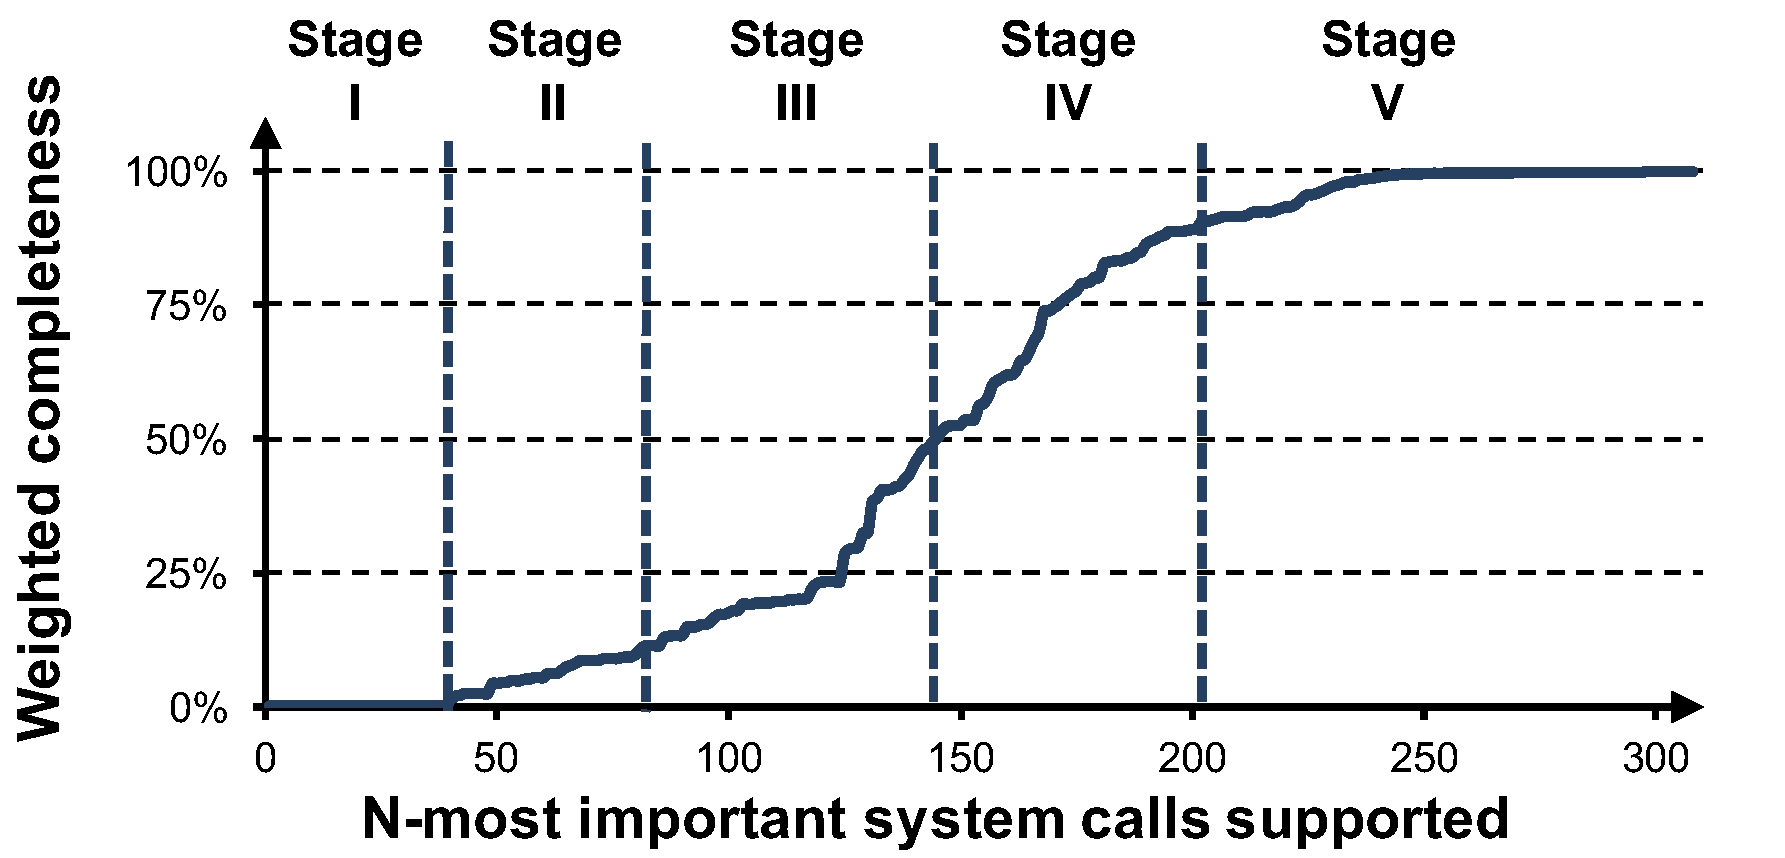
\includegraphics[width=.8\textwidth]{syscall-compatibility.pdf}
\caption{Accumulated \compatmetric{} when N top-ranked system calls are implemented in the OS. Higher is more compliant.}
\label{fig:syscall-compatibility}
\end{figure}

\begin{table}[t]
\center{
\begin{tabular}{c>{\footnotesize\raggedright\arraybackslash}m{.5\textwidth}>{\raggedleft}m{.15\textwidth}>{\raggedleft\arraybackslash}m{.15\textwidth}}
\toprule
Stage & {\normalsize Sample System Calls} & \# syscalls & {\footnotesize \CompatMetric{}} \\
\addlinespace
\midrule
I &
{\tt mmap}, {\tt vfork}, {\tt exit}, {\tt read},
{\tt gettid}, {\tt fcntl}, {\tt getcwd}
{\tt sched\_yield}, {\tt kill}, {\tt dup2}
& 40 & 1.12 \% \\
\midrule
II &
{\tt mremap}, {\tt ioctl}, {\tt access}, {\tt socket},
{\tt poll}, {\tt recvmsg}, {\tt dup},
{\tt unlink}, {\tt wait4}, {\tt select}, {\tt chdir}, {\tt pipe}
& +41 (81) & 10.68 \% \\
\midrule
III &
{\tt sigaltstack}, {\tt shutdown}, {\tt symlink},
{\tt alarm}, {\tt listen}, {\tt pread64}, {\tt getxattr}, 
{\tt shmget}, {\tt epoll\_wait},
{\tt chroot}
& +64 (145) & 50.09 \% \\
\midrule
IV &
{\tt flock}, {\tt semget}, {\tt ppoll},
{\tt mount}, {\tt brk}, {\tt pause},
{\tt clock\_gettime}, {\tt getpgid}, {\tt settimeofday},
{\tt capset}
& +57 (202) & 90.61 \% \\
\midrule
V & {\normalsize All remaining} & +70 (272) & 100 \% \\
\bottomrule
\end{tabular}
}
\footnotesize
\caption[Proposed steps of Linux system call implemetation prioritzed by importance]
{Five stages of implementing system calls based on the \usagemetric{} ranking. For each stage, a set of system calls is listed, with the work needed to accomplish (\# of system calls) and the \compatmetric{} that can be reached.}
\label{table:syscall-stage}
\end{table}

Table~\ref{table:syscall-stage} breaks down the recommended development phases by rough categories of required system calls.
We do not provide a complete ordered list here in the interest of brevity, but this list is available as part of our dataset, 
at \projecturl{}.

A goal of \compatmetric{} is to help guide the process of developing new system prototypes.
Section~\ref{sec:observation:syscall} showed that 224 out of \syscallnum{} system calls on \osdist{} have 100\% \usagemetric{}.
In other words, if one of these 224 calls is missing, at least one application on a typical system will not work.
\Compatmetric{}, however, is more forgiving, as
it tries to capture the fraction of a typical installation that could work.
Only 
40 system calls are needed to have \compatmetric{} more than 1\%.
%However, to achieve non-zero \compatmetric{} to \osdist{}, it does not require a system to support all 226 system calls;
%only 
%% The reason of such a gap is that \usagemetric{} is
%% a metric more sensitive to the API usage of individual applications:
%% as long as at least one application in every installation uses
%% a specific API, its \usagemetric{} will be 100\%.
%% \compatmetric{} is a metric made relatively relaxed:
%% this metric evaluates the expected fraction of any installation that can be supported,
%% to provide meaningful measurements

%\callout{It takes the most effort to support first and last 10\%
%of any installation (0--10\% and 90--100\% \compatmetric{}).
%The gain in functionality is precipitous when adding the 81st--202nd system calls.}

For simplicity, Table~\ref{table:syscall-stage}
only includes system calls, % \compatmetric{} based on system ,
but one can construct a similar path including other APIs, % the metric also considers other APIs,
such as vectored system calls, pseudo-files and library APIs.
For example, developers need not implement every operation of
{\tt ioctl}, {\tt fcntl} and {\tt prctl}
during the early stage of developing a system prototype.
%\fixmedp{Would it make sense to do this after the ioctls and files are covered, and include important ioctls and files?  Also, check my rewrite}

%\fixmedp{This callout is not really justified by the text  I took the point to be that the right 132 and 202 system calls are ``sweet spots'' on the path to maturity.}

\subsection{Vectored System Calls}
\label{sec:syspop:study:vector}

%\fixmedp{I think RD is right: can we give more landscape of what the long tail of vectored calls are for?  Why do they exist?}

Some system calls, such as {\tt ioctl}, {\tt fcntl},
and {\tt prctl}, essentially export a secondary system call table, 
using the first argument as an operation code.
These {\it vectored} system calls significantly expand the system API, 
dramatically increasing the effort to realize full API compatibility.
%and essentially make it harder to implement a compatibility layer.
It is also difficult to enforce robust security policies on these interfaces,
as the arguments to each operation are highly variable.
%\fixmedp{Can we comment on what, say SELinux or AppArmor actually do with ioctl?}


The main expansion is from {\tt ioctl}.
Linux defines 635 operation codes, and 
Linux kernel modules and drivers can define additional operations.
In the case of {\tt ioctl}, we obverse that there are 52 operations with the 100\% \usagemetric{} (Figure~\ref{fig:syspop:opcode-popularity}),
each of which are as important as the 226 most important system calls.
Of these 52 operations,  47 are frequently used operations for TTY console (e.g., {\tt TCGETS}) or generic operations on IO devices (e.g., {\tt FIONREAD}).

%A narrow vectored system call like {\tt fcntl} has eighteen operations in , and {\tt prctl} has 44 operations so far.
%A wider vectored system call like 
%which are further 



On the narrow end, {\tt fcntl} and {\tt prctl} have 18 and 44 operations, respectively, in Linux kernel \kernelversion{}.
Unlike {\tt ioctl}, {\tt fcntl} and {\tt prctl} are not extensible by modules or drivers,
and their operations tend to have higher \usagemetric{} (Figure~\ref{fig:syspop:opcode-popularity}).
For {\tt fcntl}, eleven out of eighteen {\tt fcntl} operations in Linux \kernelversion{} have \usagemetric{} at around 100\%.
For {\tt prctl}, only nine out of 44 operations have \usagemetric{} around 100\%,
and only eighteen has \usagemetric{} larger than 20\%.
%Because of the more equally important operations, {\tt fcntl} is a less urgent target for reformation, while {\tt prctl} has plenty of unused or infrequently used read-only operations that can be moved to pseudo-file system interfaces like {\tt /proc}.


Thus, developers of a new system prototype should support these 47 most important {\tt ioctl}
operations, about half of the {\tt fcntl} opcodes, and only 9--20 {\tt prcntl} operations.


%% Although the 47-most important ioctl operations have 100\% \usagemetric{},
%% promoting any of these operations to system calls is not beneficial.
%% Vectored system calls with limited amounts of operation codes
%% are almost equally easy to secure and maintain
%% as normal system calls.
%% However the disruptiveness of removing these operations codes
%% is unbearable for applications. 

%% However, knowing the most important operations for vectored system calls,
%% developers of new system prototypes can choose to
%% implement only part of these vectored system calls to obtain significant improvement on \compatmetric{}.
%% %For instance, Graphene library OS~\citep{tsai14graphene} only implements {\tt FIONREAD} of {\tt ioctl} to satisfy the most common usage in applications. 

%\callout{In building a prototype system, a relatively small set of operations
%in vectored system calls are essential.}
%Highly important operations in vectored system calls
%can be implemented first, to achieve better \compatmetric{}
%with partial support of these system calls.}}

%These operations are candidates for promotion to standalone system calls,
%for better usability, more attention for their security, and ease of filtering.  

%\callout{The most ubiquitous vector operations should be upgraded to system calls.}


Compared to system calls, 
{\tt ioctl} has a much longer tail of infrequently used operations.
Out of 635 {\tt ioctl} operation codes defined by modules or drivers hosted in Linux kernel \kernelversion{},
only 188 have \usagemetric{} more than one percent,
and for only 280 we can find usage of the operations in at least one application binary.
Those unused operations are good targets for deprecation, in the interest
of reducing the system attack surface.
%since leaving them around causes the OS open to attacks if any vulnerabilities exist in these APIs.
%\fixmetsai{What can we find out in this long tail?}

%\callout{{\tt ioctl} system call has a very long tail of unused operations, which may create system security risks.}

\begin{figure}[t]
\centering
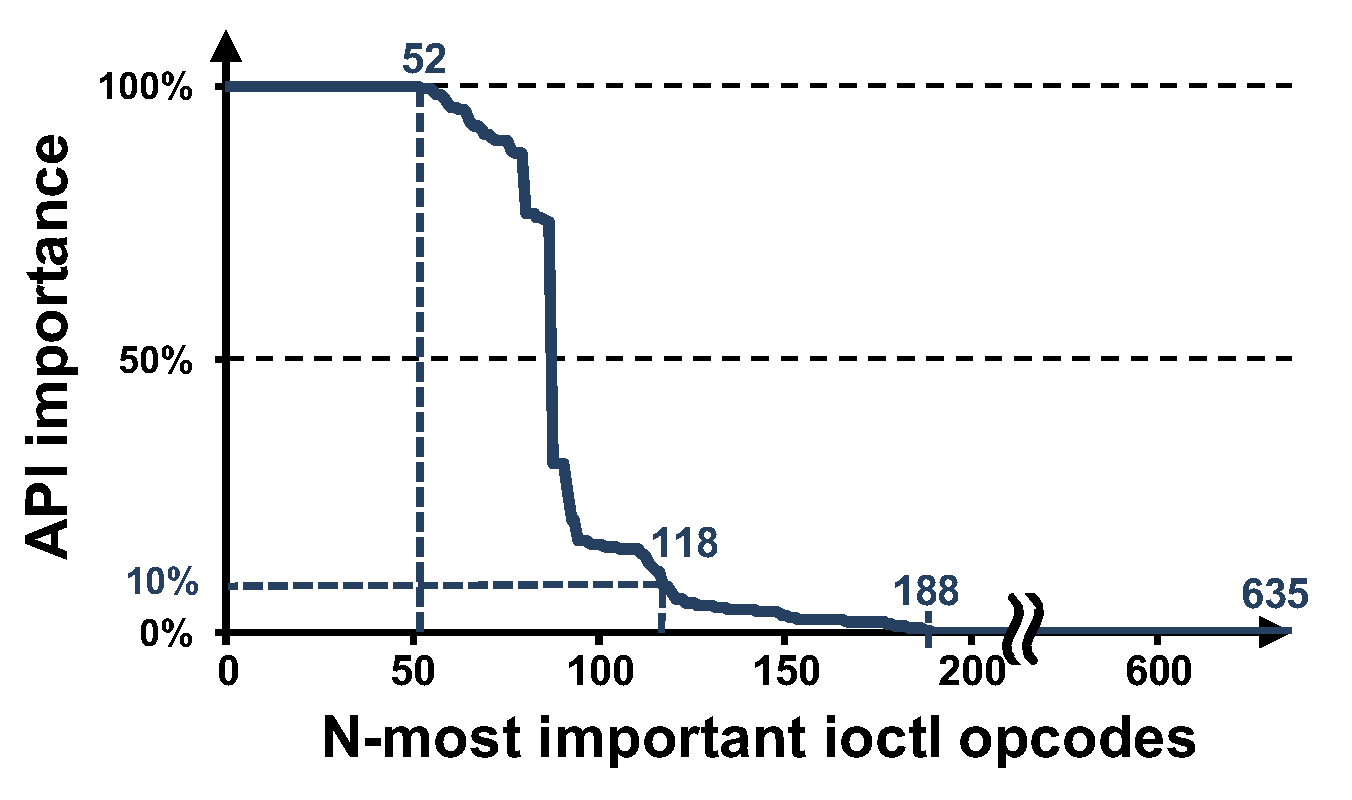
\includegraphics[width=.48\textwidth]{ioctl-popularity-by-inst.pdf}
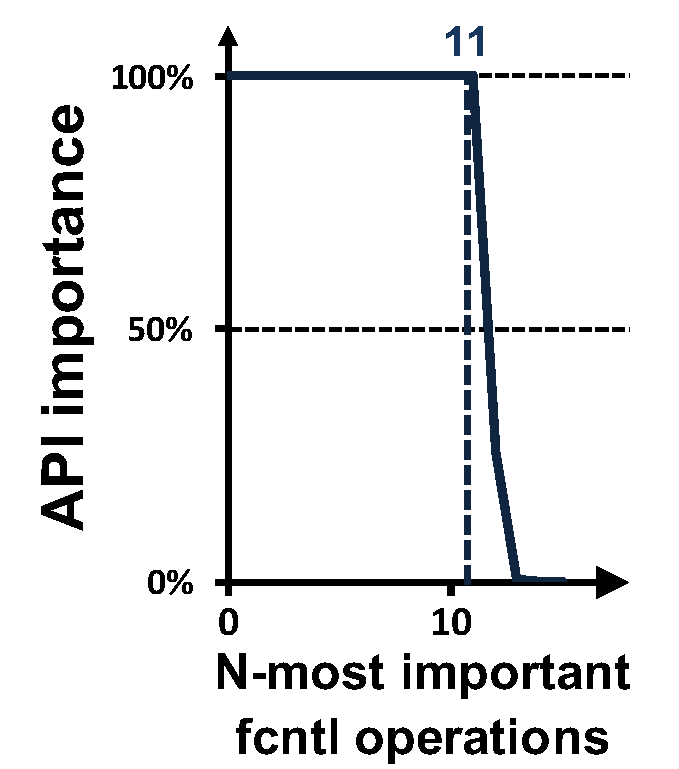
\includegraphics[width=.25\textwidth]{fcntl-popularity-by-inst.pdf}
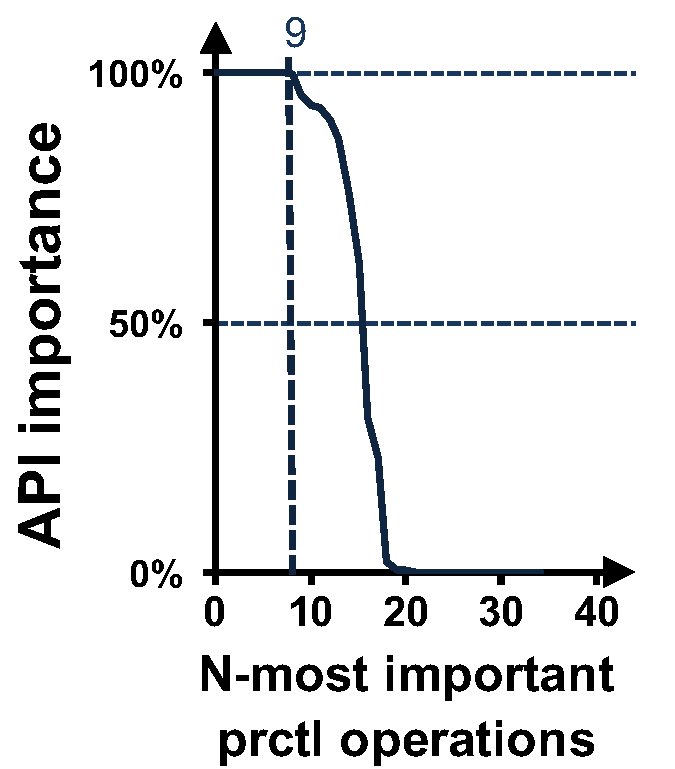
\includegraphics[width=.25\textwidth]{prctl-popularity-by-inst.pdf}
\caption{Ranking of \usagemetric{} among {ioctl}, {\tt fcntl} and {\tt prctl} opcodes.  Higher is more important; 100\% indicates all installations include software that request the operations.}
\label{fig:syspop:opcode-popularity}
\end{figure}


%\fixmedp{If time, it would be nice to investigate these zero cases and make sure no one really uses them}

%\begin{figure}[t]
%\center{
%\includegraphics[width=0.95\linewidth]{figures/fcntl-popularity.pdf}
%}
%\footnotesize
%\caption{Ranking of \usagemetric{} among {\tt fcntl} commands.}
%\label{fig:fcntl-popularity}
%\end{figure}

%\begin{figure}[t]
%\center{
%\includegraphics[width=0.95\linewidth]{figures/prctl-popularity.pdf}
%}
%\footnotesize
%\caption{Ranking of \usagemetric{} among {\tt prctl} codes.}
%\label{fig:prctl-popularity}
%\end{figure}

\subsection{Pseudo-Files and Devices}
\label{sec:syspop:study:pseudo}

In addition to the main system call table, Linux exports many additional APIs through 
pseudo-file systems, such as {\tt /proc}, {\tt /dev}, and {\tt /sys}.
These are called pseudo-file systems because they are not backed by disk, but
rather export the contents of kernel data structures to an application or administrator
as if they were stored in a file.
These pseudo-file systems are a convenient location to export tuning parameters, statistics, 
and other subsystem-specific or device-specific APIs.
Although many of these pseudo-files are used on the command line or in scripts by an administrator,
a few are routinely used by applications.
% interfaces are often the last resort of APIs, for accommodation of the most exotic interfaces. 
In order to fully understand usage patterns of the Linux kernel, pseudo-files must also be considered.

We apply static analysis to find cases where the binary is hard-coded to use a pseudo-file.
Our analysis cannot capture cases where a path to one of these file systems is passed as 
an input to the application, such as {\tt dd if=/dev/zero}.
However, when a pseudo-file is widely-used as a replacement for a system call,
these paths tend to be hard-coded in the binary as a string or string pattern.
%most instances of these file systems as system call replacements have hard-coded paths or patterns 
%in the binary.  
A common pattern we observed was {\tt sprintf(``/proc/\%d/cmdline'', pid)}; our analysis captured these patterns as well.
We also do not differentiate types of access in this study, such as separating read
versus write of a pseudo-file; rather we only consider whether the file is accessed or not.
Thus, our analysis is limited to strings stored in the binary, but we believe this captures
an important usage pattern.  %is a reasonable sample.


%% Note that matching hard-coded paths in binaries does not differentiate
%% the type of access on the files or devices.
%% The possible access on a pseudo file includes reading or writing data, retrieving file attributes, waiting on file descriptor events,
%% or performing directory operations.
%% Our study treat all access to one particular pseudo-file or device
%% as using the same API.

\begin{figure}[t]
\centering
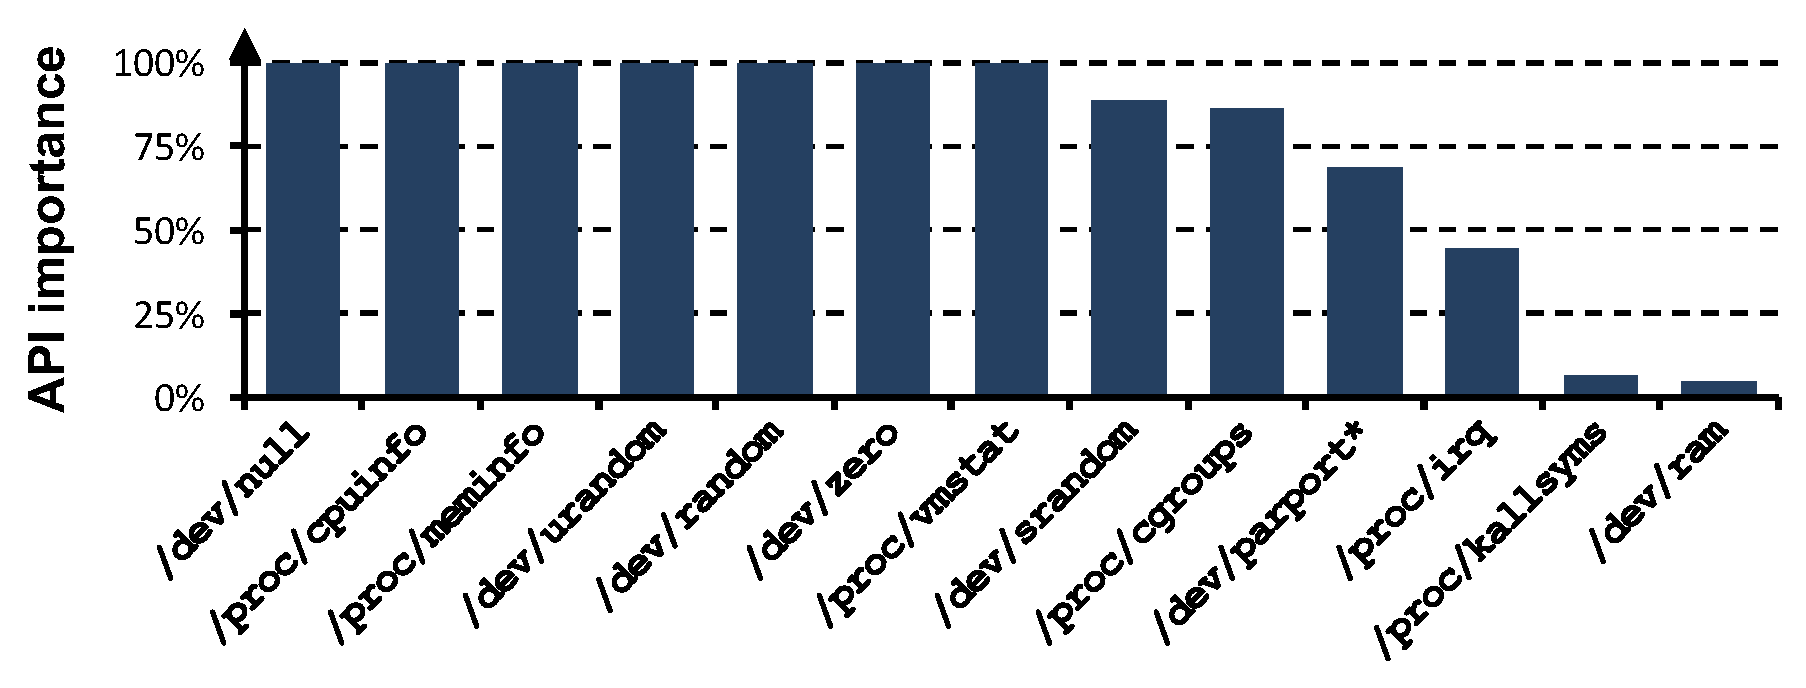
\includegraphics[width=5.5in]{syspop/figures/dev-proc-popularity-by-inst.pdf}
\caption{\usagemetric{} distribution over files under {\tt /dev} and {\tt /proc}.  Higher is more important; 100\% indicates all installations include software that accesses the file. }
\label{fig:syspop:dev-proc-popularity}
\end{figure}

Figure~\ref{fig:syspop:dev-proc-popularity} shows the \usagemetric{} of common pseudo-files under {\tt/dev} and {\tt /proc}.  
These files are ordered from highest \usagemetric{}; the long tail
of files used rarely or directly by administrators is omitted.

%There are two striking facets of this data.
Some files %under {\tt /proc} and {\tt /dev}
are essential,
such as {\tt /dev/null} and {\tt /proc\-/\-cpuinfo}.
These files are widely used in %are hard to deprecate because the usage of
%these APIs exists in not only 
binaries and scripts.
%\fixmedp{Can we comment on how many apps or libraries include a hard-coded string or pattern?}
Among 12,039 binaries that use a hard-coded path,
3,324 access {\tt /dev/null} and 439 access {\tt /proc/cpuinfo}.
However, it is plausible to provide the same functionality in
simpler ways.
For instance, {\tt /proc/cpuinfo} provides a formatted wrapper for
the {\tt cpuinfo} instruction, which one could export
directly to userspace using virtualization hardware, similar to Dune~\citep{belay12dune}.
Similarly, {\tt /dev/zero} or {\tt /dev/null} are convenient for use on the command
line, but it is surprising that a significant number of applications
issue {\tt read} or {\tt write} system calls, rather than simply zeroing a buffer
or skipping the {\tt write}
(e.g., {\tt grub-install}).
%\fixmedp{Can we offer concrete examples of apps that do this?}
Thus, in implementing a Linux compatibility layer, a small number of pseudo-files
are essential, and perhaps others could be eliminated with modest application changes.


%% provide more security-aware alternatives
%% to these APIs, so security-sensitive applications
%% can remove the usage to reduce their attack surfaces.}
%% %These system calls can be either repromoted to system call interfaces,
%% %or directly served inside system libraries using a library OS approach,
%% %to avoid increasing API footprint.
%% For example, \libc{} can encapsulate {\tt /dev/null} and serve it in the user space.
%% %without the usage of real system calls.
%% {\tt /proc/cpuinfo} can be stored as a static information in user's memory,
%% or retrieved from CPU using the {\tt CPUINFO} instruction.

APIs as pseudo-files or pseudo-devices also have a large subset
of infrequently used or unused APIs.
%Second, pseudo-file systems contain a large collection of APIs that are infrequently used,
Many of them
are designed to support one specific application or user.
%only serve certain special purposes for few applications or end-users
For example, {\tt /dev/kvm} is only intended for {\tt qemu} to
communicate with the kernel portion of the KVM hypervisor.
Similarly {\tt /proc/kallsyms} is used primarily to export debugging information to kernel developers.

Because so many files in {\tt /proc} are accessed from the command line
or by only a single application, it is hard to conclude that any should be deprecated.
Nonetheless, these files represent large and complex APIs that create an important attack surface to defend.
As noted in other studies, the permission on {\tt /proc} tend to be
set liberally enough to leak a  significant amount of information~\citep{memento}.
%\fixmedp{Can we comment on how many of these are really accessible from regular applications/ how used in SELinux/AppArmor}
For files used by a single application, an abstraction like a fine-grained capability~\citep{shapiro99eros}
might better capture this need.  
%\fixmedp{I think kvm actually does use some sort of capability already. Please check.}
For files used primarily by the administrator,
carefully setting directory permissions should be sufficient.
%, but with careful consideration of using any security-enhanced Linux variant.



%% Although cleaning up the unused APIs is beneficial for the cleanness of the system design,
%% because pseudo-files and pseudo-devices are often considered
%% the last resort of APIs,
%% developers may choose not to deprecate them.
%% %there is no reason to deprecate them or delegate them to other interfaces
%% %if OS maintainers still consider the APIs useful.
%% %For example, {\tt /proc/kallsyms}
%% %only has \usagemetric{} less then ten percent,
%% %but it is
%% %a necessary API for Linux kernel development.
%% Instead of deprecating unused API,
%% we can apply more secure mechanisms, such as AppArmor or SELinux,
%% to restrict the access to particular applications.}
%% %to prevent them from becoming system vulnerabilities. 

%\callout{A few pseudo-files are essential and must be implemented
%by any Linux-emulator.  Most serve a specific purpose, and might benefit
%from stricter enforcement of the principle of least privilege.}

%For pseudo-files and devices that are ubiquitously important, system developers should provide more secure alternatives
%if possible. Infrequently used APIs that are important for particular applicatins need to be further secured.}}

%First, the \usagemetric{} of these file under {\tt /proc} is very bimodal.
%There are over 1,000 files that are not directly used by any application; we expect that most of these
%are interfaces for an administrator to adjust kernel behavior.

%Second, there are 148 files with an \usagemetric{} score above 90\%---almost as many as there are system calls with a similar \usagemetric{} score.

%\fixme{Remove the discussion about performance impact for now. Will resurrect it after I confirm it is true.}
%In some cases, libraries or applications can tolerate a missing {\tt /proc} file
%by falling back to default values or alternate interfaces.
%For instance, {\tt gcc} will try to read {\tt /proc/cpuinfo} to guide its selection of optimizations and {\tt /proc/meminfo} to avoid
%swapping; if this file is not available, 
%{\tt gcc} will use default values.
%Our static analysis does not detect these cases.
%Nonetheless, in building a Linux-compatibility system, whether these pseudo-files are accurately 
%emulated can have a first-order impact on performance.
%In our experience building the Graphene library OS~\citep{tsai14graphene}, {\tt gcc}
%performance \fixmedp{data nugget here}.

%developers interested in emulating Linux or similar systems should carefully evaluate their emulation of {\tt /proc}.

In the case of the {\tt /dev} file system, the most commonly used files are pseudo-devices, such as accessing
the virtual terminal ({\tt /dev/tty}, {\tt /dev/console}, and {\tt /dev/pts}), or other functionality 
such as the random number generator ({\tt /dev/urandom}).
Even among pseudo-devices, features such as accessing one's standard in and out, or a process's TTY
via the {\tt /dev/} interface are not heavily used.

Intuitively, one would not expect many device paths to be hard-coded, and most direct interactions 
with a device would be done using administrative tools.
For instance, we see that some applications do hard-code paths like {\tt /dev/hda} (commonly used for an IDE hard drive),
yet an increasing number of systems have a root hard drive using SATA, which would consequently be named {\tt /dev/sda}.
Thus, although applications may use paths like {\tt /dev/hda} as a default device path, modern systems are sufficiently varied
that these generally need to be searched at runtime.

%\begin{figure}[t]
%\centering
%\includegraphics[width=0.9\linewidth]{figures/sys-popularity.pdf}
%\caption{\usagemetric{} distribution over the set of files under {\tt /%sys}.  Higher is more heavily used; 1 indicates all systems include %software that accesses the file. }
%\label{fig:sys-popularity}
%\end{figure}

%In the case of {\tt /sys} (Figure~\ref{fig:sys-popularity}), 
%we again note that there are 63 paths with a \usagemetric{} value above 90\%,
%and a total of 97 above 20\%.  Several of these export CPU or power management features,
%or user-accessed buses, like USB.  Unlike {\tt /dev}, several of these hard-coded files 
%are also actual (expected) devices, such as PCMCIA devices.

%Table~\fixmedp{XX} lists the {\tt /proc} files with a \usagemetric{} score of one.  
%\fixmedp{What else to say about this?  Might be more interesting to know how ubiquitously used these are}

\subsection{\Libc{} functions}
\label{sec:syspop:study:libc}

In addition to studying kernel interfaces, we also analyze the \usagemetric{} of APIs
defined in core system libraries, such as \libc{}.
Most programmers don't directly use the APIs exported by the kernel,
but instead program to more user-friendly APIs in \libc{} and other libraries.
%The \libc{} implementation contains lots of wrappers,
%or more user-friendly API variants of system calls and others.
For instance, \glibc{}~\citep{glibc} exports APIs for using locks and condition variables, which internally 
use the subtle {\tt futex} system call~\citep{franke02futex}.

%Figure~\ref{fig:syspop:libc-popularity} 
Our result shows that among %shows the \usagemetric{} of 
the global function symbols exported by 
\libc{} --- 1,274 in total % API among all packages. 
%Here we define \libc{} API as functions that are exported as global function symbols in \libc{}.
%The definition yields a total of 1,274  APIs,
%Among these APIs,
--- 42.8\% have a \usagemetric{} of 100\%,
50.6\% have a \usagemetric{} of less than 50\%,
and 39.7\% have a \usagemetric{} of less than one percent, including some that are not used at all.
In other words, about 40\% of the APIs inside \libc{}
are either not used or only used by few applications.
This result implies that most processes are loading a significant amount of 
unnecessary code into their address space.
By splitting \libc{} into several sub-libraries, based on \usagemetric{}
and common linking patterns, systems could realize a non-trivial space savings.

%\fixmedp{Can we assert that important and unimportant APIs are interleaved
%  on the same pages, so lazy loading doesn't help?}
There are several reasons to avoid loading extra code into an application.
First, there are code reuse attacks, such as return-oriented programming (ROP)~\citep{return-oriented},
that rely on the ability to find particular code snippets, called gadgets.
Littering a process with extra gadgets offers needless assistance to an attacker.
Similarly, when important and unimportant APIs are on the same page,
memory is wasted.  
Finally, the space overhead of large, unused jump tables is significant.
In \glibc{} 2.21, {\tt libc-2.21.so} essentially has 1274 relocation entries, occupying 30,576 bytes of virtual memory. 
%\fixmedp{true?: Because important and unimportant APIs are interleaved, all of these pages typically demand-allocated, even for applications that only use the most popular entries.}
By sorting the relocation table according to API usage,
most \libc{} instances could load only first few pages of relocation tables, and leave the remaining relocation entries for lazy loading.

We analyzed the space savings of a 
\glibc{} 2.21 which removed any APIs with \usagemetric{} lower than 90\%.
In total, \libc{} would retain 889 APIs
and the size would be reduced to 63\% of its original size.
%to \libc\_minor (in total  will stay in \libc{}).
%The size of \libc{} is reduced to 
The probability an application would need a missing function and load it from another library is less than 9.3\%(equivalent to 90.7\% \compatmetric{} for the stripped \libc{}).
%and the probability of any application loading \libc\_minor is smaller than 9.3\% 
Further decomposition is also possible, 
such as placing APIs
that are commonly accessed by the same application into the same sub-library.

%% Knowing the usage of \libc{} APIs, developers can decompose
%% a large \libc{} binary into smaller libraries.
%% Breaking down the size of \libc{} binary effectively reduces
%% the security threats in \libc{},
%% such as the risk of ROP (Return-Oriented Programming) attack.
%% The simplest way of decomposing \libc{} is
%% to move all APIs with lower \usagemetric{}
%% to another library \libc\_minor.


%It could reduce effective memory footprint to deprecate the functions that are never used, 
%or move rarely-used APIs into a separate library. % additional libraries so they do not have to be loaded or installed all the time.

%% \rev{Transition}{Another minor benefit of decomposing \libc{}
%% or just re-ordering \libc{} APIs
%% is to optimize the resource usage needed for dynamic loading of these APIs.}
%% %Other usage of this statistics is to provide them to compilers as a hint to optimize the dynamic loading.
%% Dynamic libraries like \libc{} are relocated during loading time
%% of user processes,
%% and the virtual memory used for storing relocation tables for
%% all libraries loaded in all user processes can be a non-trivial memory footprint because they are unable to share physical pages.
%% In \glibc{} 2.21, {\tt libc-2.21.so} essentially has 1274 relocation entries, occupying 30,576 bytes of virtual memory. 
%% By sorting the relocation table according to API usage,
%% Most \libc{} can load only first few pages of relocation tables, and leave the remaining relocation entries for lazy loading.

%\callout{Decomposing or re-ordering library API can lower memory costs
%in typical application processes.}
%API usage statistics are hints for compilers to optimize memory footprint of dynamic loading by sorting relocation tables by \usagemetric

%\begin{figure}[t]
%\centering
%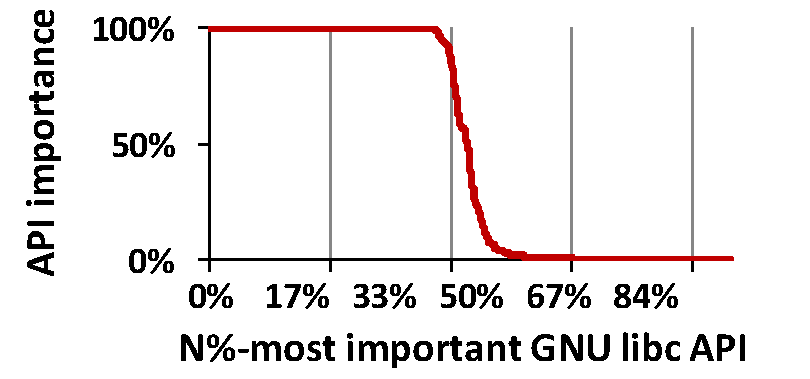
\includegraphics[width=3.6in]{syspop/figures/libc-popularity.pdf}
%\caption[\Usagemetric{} distribution of GNU Library C functions]
%{\usagemetric{} distribution over the set of GNU Library C. Higher is more important; 100\% indicates all installations include software that use the \libc{} API. }
%\label{fig:libc-popularity}
%\end{figure}

%%%We observe that majority (xx \%) of the executables in the \osdist{} repository are ELF binaries (Figure~\ref{fig:executable-type}).
%%%The other executables rely on interpreters like shell, perl, python, etc. We focus our study
%%%only on the ELF binaries which also include the interpreters for other scripts. However, we do
%%%not use the scripts popularity and their footprint while calculating the metric for system call popularity.
%%%Overall, in order to get a compatibility score with Linux for any given OS, we calculate popularity of 4 different
%%%interfaces that the applications use.

\paragraph{Effects of standard libraries on \usagemetric{}.} \Libc{} and the dynamic linker ({\tt ld.so}) 
also contribute to the system call footprint of every dynamically-linked executable.
This has a marked effect on the \usagemetric{} of some system calls.
The APIs used to initialize a program  are listed in Table~\ref{table:libc-init-call}.
In several cases, such as {\tt set\_tid\_address}, however, \libc{} or \libpthread{} may be the only binaries using these interfaces directly,
indicating that changes to some important system interfaces would only require changes in one or two low-level libraries.

%\callout{GNU Library C and the dynamic linker can have a first-order effect on the \usagemetric{} of some system calls.}

%%% \begin{compactenum}
%%% \item Users and developers are often unaware of the footprint caused inside initialization and finalization of \libc{}. For library APIs, users at least have basic sense about what the footprint may look like.
%%% \item It requires only minimal effort to maintain compatibility between GNU Library C and kernel, because the development is actually closely coupled. 
%%% \end{compactenum}
 

%%% These APIs are also the fundamental API footprint of a {\tt Hello World} program.
%%% The developers of GNU C library made the choice of relying on certain APIs, making them one of the most important in the system. 

%%% For example, in our study, the usage in \libc{} has increased the \usagemetric{} of system call {\tt set\_tid\_address} by 0.75, suggesting that deprecating the system call will takes only little effort but changing {\em libc} itself.    

\begin{table}[t]
\centering
\small
\begin{tabular}{>{\footnotesize\raggedright\arraybackslash}m{.6\textwidth}>{\raggedright\arraybackslash}m{.3\textwidth}}
\hline
\addlinespace
System Calls & Libraries \\
\addlinespace
\hline
{\tt access}, {\tt arch\_prctl}, {\tt mprotect} & ld.so \\
\hline
{\tt clone}, {\tt execve}, {\tt getuid}, {\tt gettid},
{\tt kill}, {\tt getrlimit}, {\tt setresuid} & libc \\
\hline
{\tt close}, {\tt exit}, {\tt exit\_group}, {\tt getcwd},
{\tt getdents}, {\tt getpid}, {\tt lseek}, {\tt lstat},
{\tt mmap}, {\tt munmap}, {\tt madvise}, {\tt mprotect},
{\tt mremap}, {\tt newfsstat}, {\tt read} &
libc, ld.so \\
\hline
{\tt rt\_sigreturn}, {\tt set\_robust\_list}, {\tt set\_tid\_address} &
libpthread \\
\hline
{\tt rt\_sigprocmask} &
librt \\
\hline
{\tt futex} &
libc, ld.so, libpthread \\
\hline
\end{tabular}
\footnotesize
\caption{Ubiquitous system call usage caused by initialization or finalization of \libc{} family.}
\label{table:libc-init-call}
\end{table}

\section{Linux Systems and Emulation Layers}

This section uses \compatmetric{} to evaluate systems or emulation layers with partial Linux compatibility.
We also evaluate several \libc{} variants for their degree of completeness against the APIs exported by \glibc{} 2.21.

\subsection{\CompatMetric{} of Linux Systems}

\begin{table}[t]
\centering
\small
\begin{tabular}{m{0.8in}>{\centering}m{1in}>{\raggedright\arraybackslash\footnotesize}m{3.2in}>{\raggedleft\arraybackslash}m{0.8in}}
\toprule
Systems & \# & Suggested APIs to add & W.Comp. \\
\midrule
\addlinespace
UML \kernelversion{} & 284 & {\tt name\_to\_handle\_at}, {\tt iopl}, {\tt ioperm}, {\tt perf\_event\_open} & 93.1\% \\
\addlinespace
\hline
\addlinespace
L4Linux 4.3 & 286 & {\tt quotactl}, {\tt migrate\_pages}, {\tt kexec\_load} & 99.3\% \\
\addlinespace
\hline
\addlinespace
FreeBSD-emu 10.2 & 225 & {\tt inotify}*, {\tt splice}, {\tt umount2}, {\tt timerfd}* & 62.3\% \\
\addlinespace
\hline
\addlinespace
Graphene  & 143 & {\tt sched\_setscheduler}, {\tt sched\_setparam} & 0.42\% \\
Graphene\textsuperscript{\P} & 145 & {\tt statfs}, {\tt utimes}, {\tt getxattr}, {\tt fallocate}, {\tt eventfd2} & 21.1\% \\
\end{tabular}
\caption{\Compatmetric{} of several Linux systems or emulation layers. For each system, we manually identify the number of supported system calls (``\#''), and calculate the \compatmetric{} (``W.Comp.'') . Based on \usagemetric{}, we suggest the most important APIs to add.
(*: system call family.
\P: Graphene after adding two more system calls.) }
\label{tab:linux-compat}
\end{table}

To evaluate the \compatmetric{} of Linux systems or emulation layers,
the prerequisite is to identify the supported APIs of the target systems.
Due to the complexity of Linux APIs and system implementation,
it is hard to automate the process of identification.
However, OS developers are mostly able to maintain such a list based on the internal knowledge. 

We evaluate the \compatmetric{} of four Linux-compatible systems or emulation layers:
User-Mode-Linux~\citep{user-mode-linux}, L4Linux~\citep{hartig97mu}, FreeBSD emulation layer~\citep{freebsd-emu}, and Graphene library OS~\citep{tsai14graphene}.
For each system, we explore techniques
to help identifying the supported system calls,
based on how the system is built.
For example, User-Mode-Linux and L4Linux
are built by modifying the Linux source code,
or adding a new architecture to Linux.
These systems will define architecture-specific system call tables,
and reimplement {\tt sys\_*} functions in the Linux source
that are originally aliases to {\tt sys\_ni\_syscall}
(a function that returns {\tt -ENOSYS}). 
Other systems, like FreeBSD and Graphene,
are built from scratch,
and often maintain their own system call table structures,
where unsupported systems calls
are redirected to dummy callbacks.

%Because the evaluation is simply a proof-of-the-concept,
%we count only system calls,
%omitting other APIs such as vectored system calls and pseudo-files. 

Table~\ref{tab:linux-compat} shows \compatmetric{},
considering only system calls.
The results also identify the most important system calls
that the developers should consider adding. 
User-Mode-Linux and L4Linux both have a \compatmetric{} over 90\%,
with more than 280 system calls implemented.
FreeBSD's  \compatmetric{} is  62.3\% because it is missing some less
important system calls
such as {\tt inotify\_init} and {\tt timerfd\_create}.
Graphene's \compatmetric{} is only 0.42\%.
We observe that the primary culprit is 
scheduling control; by adding two scheduling system calls,
Graphene's \compatmetric{} would be 21.1\%.

\subsection{\CompatMetric{} of \Libc{}}

\begin{table}[t]
\center{
\setlength{\tabcolsep}{1pt}
\small
\begin{tabular}{m{0.7in}>{\centering}m{0.4in}>{\raggedright\arraybackslash\footnotesize}m{1.1in}>{\raggedleft\arraybackslash}m{0.45in}>{\raggedleft\arraybackslash}m{0.55in}}
\toprule
\Libc{} variants & \# & Unsupported (samples) & {\footnotesize W.Comp.} & {\footnotesize W.Comp.} {\scriptsize (normalized)} \\
\midrule
\addlinespace
eglibc 2.19 & 2198 & None & 100\% & 100\% \\
\addlinespace
\hline
\addlinespace
uClibc 0.9.33 & 1867 & {\tt \_\_uflow}, {\tt \_\_overflow}  & 1.1\% & 41.9\% \\
\addlinespace
\hline
\addlinespace
musl 1.1.14 & 1890 & {\tt secure\_getenv}, {\tt random\_r} & 1.1\% & 43.2\% \\
\addlinespace
\hline
\addlinespace
dietlibc 0.33 & 962 & {\tt memalign}, {\tt stpcpy}, {\tt \_\_cxa\_finalize}  & 0\% & 0\% \\
\end{tabular}
}
\caption{\Compatmetric{} of \libc{} variants. For each variant, we calculate \compatmetric{} based on symbols directly retrieved from the binaries,
and the symbols after reversing variant-specific replacement (e.g.,{\tt printf} becomes {\tt \_\_printf\_chk}).}
\label{tab:libc-compat}
\end{table}

This study also uses \compatmetric{} to evaluate the compatibility of several \libc{} variants --- eglibc~\citep{eglibc}, uClibc~\citep{uclibc}, musl~\citep{musl} and dietlibc~\citep{dietlibc} --- against \glibc{},
listed in Table~\ref{tab:libc-compat}.
We observe that, if simply matching exported API symbols, only eglibc is directly compatible to \glibc{}.
Both uClibc and musl have a low \compatmetric{}, because \glibc{}'s headers replace a number of APIs with safer variants at compile time, using macros.
For example, \glibc{} replaces {\tt printf} with {\tt \_\_printf\_chk}, which performs an additional check for stack overflow.
%Because these new APIs often have the same interface as the old ones,
%we assume other \libc{} variants can easily
%reverse the API replacement during symbol resolution.
After normalizing for this compile-time API replacement, both uClibc and musl are at over 40\% \compatmetric{}.
In contrast, dietlibc is still not compatible with most binaries linked against \glibc{} --- if no other approach is taken to improve its compatibility.
The reason of low \compatmetric{} is that dietlibc does not implement many ubiquitously used \glibc{} APIs such as {\tt memalign} (used by 8887 packages) and {\tt \_\_cxa\_finalize} (used by 7443 packages).

\papersection{Security isolation}
\label{sec:linux:security}

\issuedone{1.1.d}{Describe the security isolation story for Linux hosts}
\graphene{} separates OS features from security isolation.
This section explains the Linux host design for isolating mutually untrusting applications, with a reduced attack surface for protecting Linux kernels.
The discussion starts with the security guarantees and threat model, followed by the technical details of security isolation on a Linux host.



\papersubsection{Goals and threat model}

The security isolation model of \graphene{} ensures that mutually-untrusting applications cannot interfere with each other.
A goal of \graphene{} is to provide security isolation with comparable strength as
running applications in separate VMs.
When running two unrelated applications on the same machine,
the security requirement
of the OS involves not only blocking unauthorized access under normal circumstance,
but also preventing an application
from maliciously exploiting OS vulnerabilities to attack the other application.
Because a modern OS, such as Linux or \win{}, contains a rich of features and APIs,
it is difficult to eliminate OS vulnerabilities
or even just to verify whether an OS contains any vulnerabilities. 
A Linux container~\cite{lxc}
does provide a separate OS view for each application,
but still relies on the correctness of the whole Linux kernel to enforce security isolation.
On the other hand, a VM or a \libos{}
isolates the whole OS kernel or a part of the kernel in an unprivileged guest space
for each application.
The security isolation model prevents
any vulnerabilities inside the VM or the \libos{} from compromising the host kernel and other applications.



\graphene{} enforces security isolation %between applications
by separating 
backward-compatible OS features from security mechanisms.
A Linux kernel exports a wide range of system calls,
either as a legacy of previous kernels or as new programmability features. % of newer kernels.
By implementing OS features in a \libos{},
\graphene{} reduces the attack surface of a Linux kernel
to a small amount of system call corner cases.
%to implement \thehostabi{}.
%If a machine only runs applications in \graphene{},
%a Linux developer can try to carve out a minimal Linux kernel, containing only features needed by the Linux PAL.
A reduced attack surface
eliminates majority of execution paths inside a Linux kernel in which a malicious application can explore for vulnerabilities.
The complexity of Linux features and APIs exported by a \libos{} is unrelated with the attack surface of the host kernel,
unless the \libos{} asks for additional \hostapis{}.
A Linux developer can even carve out a minimal Linux kernel with only the features needed by the Linux PAL,
similar to shrinking a Linux kernel to a microkernel.
Otherwise, \graphene{} depends on the host security mechanisms to restrict a \libos{} from accessing unauthorized system calls and resources upon an unmodified Linux kernel.





The Linux PAL installs a {\bf system call filter} and a {\bf reference monitor}
for restricting the system calls, files, RPC streams, and network addresses
accessed by a \picoproc{}.
The Linux PAL requires \hostsyscallnum{} system calls in total
for implementing both required and optional \hostapis{}.
A system call filter, such as the Linux \seccomp{} filter~\cite{seccomp},
can restrict the system call access of an application
to only a small subset of all the system calls, with additional constraints on the parameters and optional flags permitted for each system call.
%The system call filter
%forbids an application from invoking any system calls
%that will interfere other \picoproc{} or increase the risk of exploitation in the host kernel.
A reference monitor further examines the arguments of permitted system calls to restrict the host resources accessed by an application, based on security policies configured in a manifest file~\cite{hunt07rethink}.
The system call filter and the reference monitor
significantly limit the ability of an untrusted \graphene{} \picoproc{} to interfere with the rest of the system,
preventing the risk of exposing any unknown vulnerabilities
on a kernel path never exercised by the system call footprint of \graphene{}.



\graphene{} contributes a multi-process security model 
based on a {\bf sandbox},
or a set of mutually-trusting \picoprocs{} running inside an isolated container.
The reference monitor permits picoprocesses within the same sandbox
to communicate over RPC streams,
allowing the \libos{} to share and coordinate any states
to create an unified OS view.
If two \picoprocs{} belong to different sandboxes,
the reference monitor will block any attempt of connecting RPC streams
between the \picoprocs{}
The access control over RPC streams
enforces an all-or-nothing security isolation model:
either two \picoprocs{} are in the same sandbox and share all the \libos{} states; or they are separated in two sandboxes and share nothing.
Even though the \libos{} instance can span its state across multiple \picoprocs{},
a host kernel needs not to examine the accesses to shared \libos{} states, but still enforces security isolation between sandboxes.




Files and network addresses
are the only host resources allowed to be shared across sandboxes,
using well-studied, explicit rules.
For sharing files, the reference monitor restricts the file access of a \picoproc{}
within a few host file or directories,
creating a restricted view of the local file system
(close to Plan 9's unionized file system views~\cite{pike90plan9}).
The file rules
in a manifest are similar to the policies of a {\bf AppArmor profile}~\cite{apparmor};
for each permitted file or directory,
a developer specifies the URI prefix and the permitted access type, either as read-only or readable-writable. %, within the target file or directory.
For sharing network addresses,
the reference monitor restricts a \picoproc{} from connecting through a local address or connecting to a remote address,
using {\bf iptables-like firewall rules}~\cite{iptablesman}.
Each network rule in a manifest
specifies the local or remote IP address and port range that a \picoproc{} is permitted to bind or connect a network socket.
The rules in a manifest file
specify a minimal list of files and network addresses that a \picoproc{} needs to access, and are largely based on existing security policies (e.g., AppArmor profiles, firewall rules).





\paragraph{Threat model (details).}
When running on a normal Linux host (without \sgx{} or other security hardware), \graphene{} assumes a trusted host kernel and reference monitor.
All the components inside the kernel space, including the \code{gipc} kernel module for bulk IPC, and the reference monitor,
are fully trusted by the other parts of the host kernel and the \graphene{} \picoprocs{}.
%which mediates all system calls with effects outside of a picoprocess's address space,
%such as file {\tt open} or network socket {\tt bind} or {\tt connect}.
On the other hand,
the host Linux kernel does not trust the \picoproc{}, including the Linux PAL, a \thelibos{} instance, \glibc{}, and the application.
The system call filter and reference monitor
initialized before an application starts running
defend the whole host kernel from malicious system calls invoked by a \picoproc{}.



All the components running within a \picoproc{}, including the Linux PAL, the \libos{} (\thelibos{}), \glibc{} libraries, and the application,
mutually trust each other. %, because all these components
%execute in the same guest address space.
Without internal sandboxing, the Linux PAL or \thelibos{}
cannot protect its internal states or control flows from an application.
Although some scenarios might require protecting the PAL or \thelibos{}
from the application,
\graphene{} only restricts the adversary
within a \picoproc{};
in other word, an adversary
only compromises the \libos{} in the same \picoproc{},
but can never interfere the host kernel 
or other unrelated \picoprocs{}.



For a multi-process application,
\graphene{} assumes that the \picoprocs{} 
%launched by the same application instance
running inside the same sandbox
trust each other and that all untrusted code run in sandboxed \picoprocs{}.
\graphene{} assumes the adversary can run arbitrary code inside
one or multiple \picoprocs within a sandbox.
The adversary can exploit any vulnerabilities in the \libos{}
or IPC protocol,
to propagate the attack to other \picoprocs{}.
\graphene{} ensures that
the adversary cannot interfere with any victim \picoprocs{}
in a separate sandbox.
A sandbox strictly isolates the coordination of \thelibos{} instances;
%if the only shared kernel abstractions are byte streams and files, 
the reference monitor ensures
that there is no writable intersection between sandboxes, so that
the adversary cannot interfere with any victim \picoprocs{}.


%%% The only processes allowed to run as standard kernel processes (non-\graphene{}) 
%%% are the reference monitor and
%%% system administration utilities that need more kernel interfaces than the \pal{} ABI provides.
%%% Ensuring that a collaborating picoprocess correctly implements
%%% some function (such as receiving a signal),
%%% as well as preventing exploitation of vulnerabilities in picoprocesses
%%% are beyond the scope of this work.

\graphene{} reduces the attack surface of the host Linux kernel, but does not change the trusted computing base; however, reducing the effective system call table size of a \picoproc{} does facilitate adoption of a smaller host kernel.
This thesis leaves the creation of a smaller host kernel for future work.

\papersubsection{System call restriction}
\label{sec:linux:security:syscall-restriction}


\graphene{} reduces the host ABI to \palcallnum{} calls
and the Linux system call footprint to \hostsyscallnum{} system calls.
To reduce the effective attack surface to a Linux host,
the Linux host restricts a \picoproc{} from accessing any system calls that are not part of the ordinary footprint of a Linux PAL.
The system call restriction on Linux focuses on blocking most of the system calls
that interferes with other processes.
The remaining permitted system calls with external effects are checked by 
the reference monitor (see Section~\ref{sec:linux:security:ref-monitor}).
 
%% dp: Meh
%%% Any picoprocess implementation 
%%% must restrict access to the host system call table,
%%% generally by blocking system calls in the host kernel~\cite{porter11drawbridge}
%%% or using {\tt ptrace}~\cite{xax}.


%The \pal{} is a host-provided library which implements \palcalls{} generic kernel ABIs,
%implemented using 
%These native system calls include {\tt ioctl} with 5 opcodes exclusively used by \graphene{} kernel extensions.

%This section describes how we adapt recent Linux sandboxing techniques 
%to \graphene{}.


%all allowed system calls with potentially external effects.

%%% For instance, an attempt to open a file will be checked by the reference monitor
%%% to see if the file is included in the sandbox definition, specified in the manifest
%%% with required permissions.
%%% Once the file handle is open, the \pal{} is then allowed to issue an {\tt mmap} or {\tt read}
%%% on the handle, as this operation can only affect the picoprocess address space
%%% or  file, which was already checked.

%Because the \pal{} is in the same address space as the application code, it is not
%trusted to enforce any security policies, and our threat model assumes that
%the \pal{} can be compromised by the adversary.
%Thus, the host kernel 
%only permits system calls that appear in the \pal{}'s source code and, through the reference monitor, further inspects calls that can have external effects.

%\begin{figure}[t!]
%\centering
%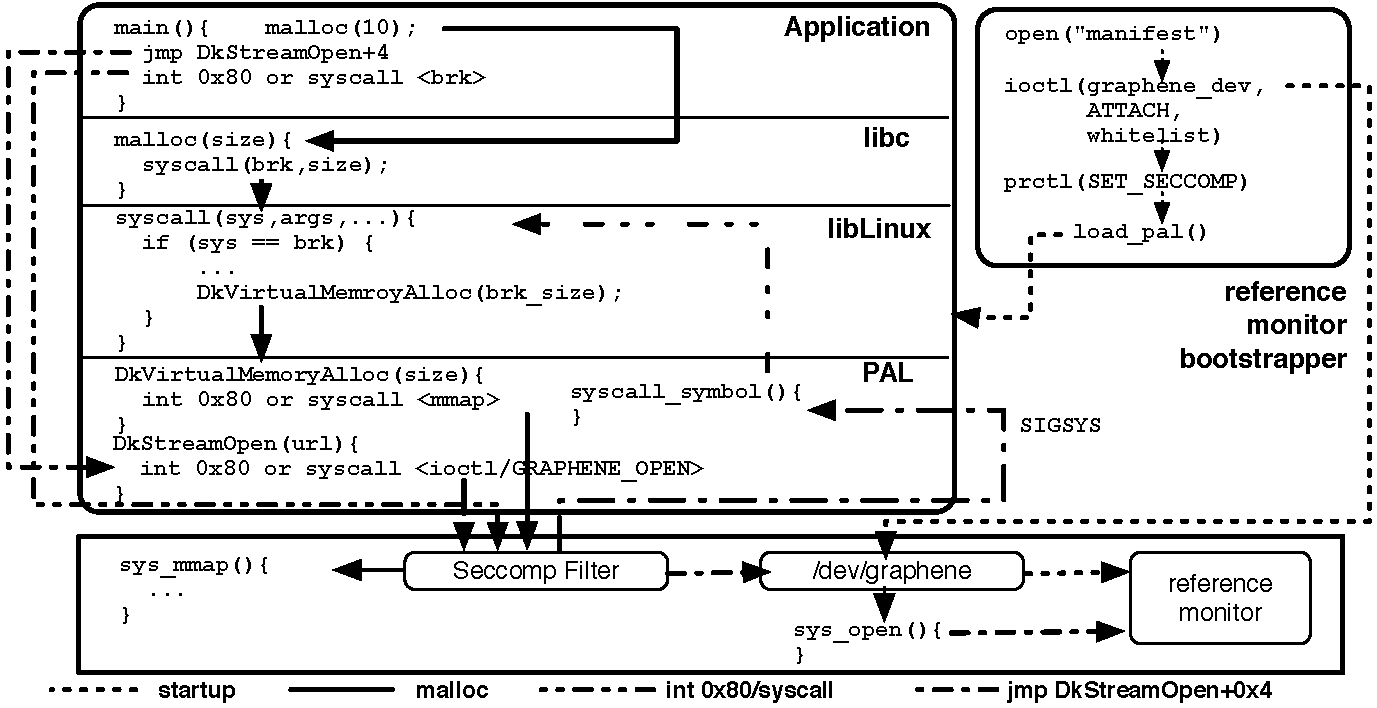
\includegraphics[width=\linewidth]{syscall-restriction.pdf}
%\footnotesize
%\caption[System call restriction approach in sysname{}]
%{System call restriction approach. The reference monitor loads policies into the LSM at startup.  A \graphene{} application requests OS services in three different ways. 
%In the normal case (first line of {\tt main}), {\tt malloc} is invoked causing the invocation of {\tt brk} ({\tt libLinux}) and {\tt mmap} in the \pal{}. In the second line, the application jumps to an address in \pal{}, which is permissible.
%Files are accessed through {\tt ioctl} to {\tt /dev/graphene} and checked by reference monitor.
%The third line invokes {\tt brk} with an {\tt int} instruction, which is redirected to the {\tt libLinux} function.}
%\label{fig:graphene:syscall-restriction}
%\end{figure}



\issuedone{1.3.d}{Extend the discussion of \seccomp{} filter}
\graphene{} restricts the host system calls 
using a \seccomp{} %(SECure COMPuting)
filter~\cite{seccomp}, a feature introduced in Linux 2.6.12.
% a recent Linux system call filtering mechanism, called 
A \seccomp{} filter allows a Linux process to install an immutable Berkeley Packet Filter (BPF) program
that specifies allowed system calls, as well as specifies
the consequence of invoking certain system calls, such as creating a \code{ptrace} event or raising a \code{SIGSYS} signal.
The BPF grammar is rich enough to filter scalar argument values,
such as only permitting specific opcodes for \syscall{ioctl},
as well as filter certain register values, such as blocking system calls from program counters (i.e., \code{RIP} register values) outside of the Linux PAL.
%This feature is particularly salient in the case of {\tt ioctl},
%where the \pal{} uses 5 out of over 400 opcodes for our bulk IPC module and sandbox creation;
%our BPF rules will block any other {\tt ioctl} opcode.
The current \seccomp{} filter installed by the Linux PAL contains \seccomplines{} lines of straightforward BPF macros.  %Experiments show that adding more precise argument checks has no significant impact on system call latency.
Once a \seccomp{} filter is installed in a process,
the filter intermediates
every system calls from the process and its future children, and guarantees the processes can never bypass the restriction.
The Linux PAL uses \code{SIGSYS} signals to capture rejected system calls,
and can either terminate the whole application or
redirect the system call to \thelibos{}.
The consecutive steps of system call redirection are described in Section~\ref{sec:libos:syscall-redirection}.



Developing a \seccomp{} filter presents several technical challenges.
First, a filter must restrict consecutive \picoprocs{}
to install a new filter the reverts the system call restriction.
%A \seccomp{} filter is installed using the \syscall{prctl} system call, so
Blocking the \syscall{prctl} system call in a \seccomp{} filter will prevent further installation of \seccomp{} filters.
Second, the BPF grammar can only filter certain values or ranges of a register.
The filter needs to
ensure that only the Linux PAL can invoke system calls;
however,
for satisfying the dynamic loading behavior of \thehostabi{},
the Linux PAL
is built as a shared library loaded at an address randomized by the Linux ASLR (Address Space Layout Randomization) feature.
If a filter only permits a specific range of program counters,
a child \picoproc{}
will load the Linux PAL at another randomized address,
and the inherited filter will restrict the child \picoproc{} to invoke any system calls.
The Linux PAL introduces a small, initial loader
loaded at a fixed address
within each \picoproc{} and permitted to invoke system calls.
Finally, a \seccomp{} filter
cannot check a string argument, such as a file path for \syscall{open} or a network address for \syscall{bind}.
Checking a string argument requires
involves reading user memory of unknown sizes and string comparison, and the BPF grammar only allows checking an argument arithmetically.
Filtering permitted file paths and network addresses
must rely on a trusted reference monitor (see Section~\ref{sec:linux:security:ref-monitor}).
%In order to avoid the overhead of trapping to the reference monitor on 
%every use of {\tt open}, {\tt stat}, {\tt bind} or {\tt connect} system calls, we instead 
%force picoprocess to only use {\tt ioctl} system call to \graphene{} special device ({\tt /dev/graphene}) as alternative interface these system calls. Direct access to these system calls are banned by seccomp filter.
%extend AppArmor~\cite{apparmor} 
%to enforce file system isolation in the kernel.



The \seccomp{} filter blocks  unauthorized system calls
from anywhere inside a \picoproc{}.
Even if none of the application binaries contains any \assembly{syscall} or \assembly{int \$80} instruction,
a piece of malicious application code can always bypass the Linux PAL
to invoke unauthorized system calls.
The application code can simply
jump to a \assembly{syscall} instruction inside the Linux PAL,
or corrupt a returned address on the current stack to launch a ROP (return-oriented programming) attack.
Even if the Linux PAL is hidden or isolated from the application,
an adversary can always leverage a gadget, a byte sequence that resembles the target instruction, within an executable or a library.
Therefore, the \seccomp{} enforces both program-counter-based 
and argument-based restrictions
to block unauthorized system calls from both the Linux PAL and the rest of \picoproc{}.


%In order to reduce the impact of bugs in the reference monitor,
%the reference monitor itself runs with a \seccomp{} filter, blocking unexpected system calls.


\paragraph{Security implications.}
Using an existing system call restriction mechanism like \seccomp{},
\graphene{} limits the ability of an untrusted application to attack a Linux kernel.
Ideally, since \thelibos{} only requires \thehostabi{},
\graphene{} can adopt a modified Linux kernel
that only exports \palcallnum{} \hostapis{} to each \picoproc{}.
%However, as a usability feature, \graphene{} runs \graphene{} on an unmodified Linux kernel using a Linux PAL to translate among host interfaces.
The \seccomp{} filter instead isolates a \picoproc{} on an unmodified Linux kernel,
with a reduced attack surface 
comparable to only exporting \thehostabi{}.
%The filter only permits \hostsyscallnum{} system calls with specific flags and opcodes
%required by the Linux PAL.
According to the principle of least privilege,
each component or layer in a system should only be granted access to a minimal amount of resources or abstractions
required for performing the expected tasks.
The \seccomp{} filter only permits
a minimal amount of system calls with specific flags and opcodes
required by the Linux PAL,
so an untrusted application
can only trigger
a limited amount of execution paths inside the host Linux kernel.
\graphene{} limits
the ability of an untrusted application to explore
known and unknown vulnerabilities
on any kernel execution paths for servicing one of the blocked system calls.



Although a regular Linux process can also leverage a \seccomp{} filter,
\graphene{} makes a major contribution
to reduce the system call footprint of any large-scale application
to a fixed, small system call profile.
Analysis %of applications and libraries
%in the official Ubuntu repositories
shows that the system call  footprint of a large-scale application such as Apache or MySQL can contain more than 100 system calls.
Since \thelibos{} has absorbed the Linux system call table,
running Apache, MySQL, or any other application in \graphene{} leads to at most \hostsyscallnum{} host system calls.
As a system
running a wide range of applications
can exposes a different partial view of the system call table to each application,
\graphene{}
has a static system call profile for all applications,
allowing OS developers to focus
on testing or analyzing a small portion of execution paths and corner cases
of a Linux kernel.
\citet{sun15unpredictability}
proposes sandboxing an uncertain, potentially-malicious application
in \graphene{}
with an unpredictable \thelibos{} implementation.







\paragraph{Static binaries.}
Besides security purposes,
a \seccomp{} filter provides a compatibility feature
for redirecting hard-coded system calls
in a statically-linked application binary.
\graphene{} leverages the \seccomp{} filter to redirect these leaked system calls
back to \thelibos{}. 
The filter contains BPF rules to check if the program counters
invoking the system calls
are parts of the Linux PAL.
The filter blocks system call invoked outside of the Linux PAL
and delivers a \code{SIGSYS} signal
to the PAL signal handler for redirecting the system calls to \thelibos{}.



\papersubsection{Reference monitor}
\label{sec:linux:security:ref-monitor}

The reference monitor on a Linux host
checks the arguments of host system calls for referencing any sharable host resources.
A host system call like \syscall{open}, \syscall{connect}, or \syscall{bind}
specifies a file system path or a network address
for opening a file or network stream and cannot be filtered by a \seccomp{} filter.
The host kernel trusts the reference monitor
to only permit
a list of sharable resources in a \picoproc{},
based on
rules in a manifest file.
Once the reference monitor has permitted the creation of a file or network stream,
consecutive operations on the stream
such as reading or writing data can be trusted
as long as being mediated by one of the permitted system calls.


\begin{figure}
\centering
\begin{lstlisting}
loader.exec = file:/usr/sbin/apache2        # allow loading executable 
loader.preload_libs = file:/graphene/libLinux.so    # loading libLinux
fs.allow_ro.libc = file:/graphene/libc/     # loading modified libc
fs.allow_ro.mods = file:/usr/lib/apache2/modules/   # loading modules
fs.allow_ro.cond = file:/etc/apache2/       # reading configuration
fs.allow_rw.logs = file:/var/log/apache2/   # writing to logs
fs.allow_ro.http_docs = file:/var/www/      # reading website files
net.allow_bind.httpd = 0.0.0.0:80           # binding to local port 80
net.allow_conn.any = 0.0.0.0:1-65535        # allow any connection
\end{lstlisting}
\caption{A example of a manifest file, containing security rules for the reference monitor to permit accessing sharable resources. The manifest file is for running a Apache http server (without php and other language engines).}
\label{fig:linux:manifest-example}
\end{figure}


The reference monitor enforces simple, white-listing rules
based on security mechanisms
already familiarized by users and developers.
Figure~\ref{fig:linux:manifest-example} shows an example of resource access rules
in a manifest.
First, a manifest lists
the URI prefixes of permitted files or directories
of an application,
similar to an AppArmor profile.
The executable (\code{loader.exec}) and the preloaded \libos{} binaries (\code{loader.preload\_libs})
are permitted for read-only access by default.
The reference monitor
simply compares file URIs against each permitted URI prefix
and checks the access types;
unlike many existing security mechanisms in Linux and similar OSes, such as permission bits, Access Control Lists (ACLs), and SELinux labels,
the reference monitor does not retrieve
security policies from file metadata, but obtains the manifest from an out-of-band channel.


Manifest-based security
simplifies the inspection, authentication, and population
of security policies.
An Android application is deployed with a similar manifest,
listing the accessed files and other resources,
which users approve when installing the application.
Developers can authenticate a security policy by signing the content of a manifest.
Moreover, to run an application, a user can choose among multiple manifest files
with different levels of security privileges.



Network rules in a manifest are similar to {\bf iptables firewall rules} for defending a server or a desktop machine.
A network rule specifies a local or remote address
that the application is permitted to bind or connect a network stream.
A local or remote address
can be an IPv4 or IPv6 address (possible to specify an ``any'' address, i.e., \code{0.0.0.0} or \code{[::1]}), combined with a specific port number or range.
When an application creates a network stream,
the reference monitor checks whether the local and remote addresses
match one of the network rules.







%is implemented using {\tt ioctl} system call to a special device {\tt /dev/graphene}.
%A picoprocess is restricted by seccomp filter~\cite{seccomp} to use any {\tt open} or socket {\tt connect} and {\tt bind} system calls.
%It must use the \graphene{} special device to open or create streams,
%so the file paths or network addresses can be checked against the sandbox rules.
%The kernel module as the driver of the \graphene{} special device can coexist with any LSM such as \emph{AppArmor} or \emph{SELinux}.

The reference monitor on a Linux host
is implemented as a Linux Security Module (LSM) extended from the existing AppArmor module.
AppArmor is the default LSM of most Linux distributions,
and a Linux kernel disallows multiple LSMs (e.g., AppArmor, SELinux) to be effective simultaneously.
\graphene{} instruments
a few security hooks of the AppArmor, to add checks for file system paths
and network addresses.
The security checks of the reference monitor are stackable with other host security mechanisms.
For example, if a manifest lists a root-privileged file and the \graphene{} application runs in a unprivileged process,
existing security checks in a Linux kernel
still blocks the file access even though the reference monitor permits the access.
The drawback of the implementation
is that \graphene{} must run on a modified Linux kernel.
Linux kernels do not support loading LSM as a dynamic kernel module.
\graphene{} only replaces
the AppArmor LSM in a Linux kernel; the rest of the Linux kernel remains unchanged.


A trusted security loader initializes the reference monitor
when launching an application in \graphene{}.
When a user launches an application in \graphene{} from the command line,
the first \picoproc{} begins in a new sandbox.
The security loader
reads the manifest file given by the user,
and submits the sandbox rules to the reference monitor.
The reference monitor exports a miscellaneous device called \code{/dev/graphene}
for the security loader to submit sandbox rules using the \syscall{ioctl} system call.
Once the reference monitor
starts a \picoproc{} in a sandbox, neither the first \picoproc{} nor any consecutive \picoprocs{} spawned in the sandbox can ever escape the sandbox or drop the restrictions on certain resources.


\paragraph{Alternative approaches.}
Other approaches can implement the reference monitor without modifying a Linux kernel, with a trade-off of performance or development simplicity.
An approach is to implement the reference monitor as a trusted process receiving \code{ptrace} events from \graphene{} \picoprocs{}.
Using the \syscall{ptrace} system call, this reference monitor can retrieve user memory from the monitored \picoprocs{},
and block the system calls which request for unpermitted resources.
Unfortunately, intercepting every system calls with \code{ptrace} events introduces significant overhead to \hostapis{};
thus, this approach is not ideal for isolating \graphene{} applications on a Linux host.


Another approach is to translate the resource rules in a manifest file
to AppArmor or iptables rules.
As explained in previous paragraph, the file and network rules in a manifest file are similar to the file lists in an AppArmor profile and the firewall rules enforced by iptables.
Instead of implementing a \graphene{}-specific reference monitor,
\graphene{} can convert a manifest file, either statically or dynamically,
to security rules recognized by AppArmor and iptables.
This approach requires no modification
in a Linux kernel, and can benefit from
existing optimizations of AppArmor and iptable. %these security mechanisms.
\graphene{} leaves the integration with AppArmor and iptables for future work.




\paragraph{Dynamic process-specific isolation.}
A child \picoproc{} may either inherit its parent's sandbox, 
or start in a new sandbox,
by either specifying a flag to \palcall{ProcessCreate} or calling the sandboxing \hostapi{}, \palcall{SandboxSetPolicy}.
A new sandbox may obtain a subset of the original file system view,
but can never request access to new regions of the 
host file system. 
%The restrictive policy enforced on the child will be written in a new manifest file generated by the parent, and the policy will be checked by the reference monitor.
If a child \picoproc{} voluntarily moves itself to a new sandbox
using \palcall{SandboxSetPolicy},
the Linux PAL issue another \syscall{ioctl} call to \code{/dev/graphene}
to dynamically detach
the \picoproc{}
from the parent's sandbox and update sandbox rules. The reference monitor
closes existing RPC streams and prevents RPC stream creation 
across sandboxes.
%among picoprocesses
%that are not in the same sandbox.
%and restricts external connections to remote URIs according to firewall rules in the manifest.
When a process detaches from a sandbox,
the reference monitor effectively splits the original sandbox
by closing any RPC streams that could bridge the two sandboxes.


\begin{comment}
We hasten to note that program counter filtering
is only provided for backwards compatibility, not security.
An attacker can compromise the \pal{}, so system policies are enforced
externally by the reference monitor.


Dynamically redirecting system calls to {\tt libLinux} is 
less efficient than dynamically linking against
the \graphene{} libc or statically compiling {\tt libLinux} into the application.
The overhead of dynamic redirection comes from 
transferring control to the kernel, then back to 
the \pal{}, and then to {\tt libLinux}.
We leave exploration of more efficient alternatives for future work,
such as redirecting the hardware system call table to {\tt libLinux}
on a host system like Dune~\cite{belay12dune},
or dynamically rewriting parts of the static binary~\cite{hunt99detours}.
\end{comment}

%\paragraph{Example.}
%Figure~\ref{fig:graphene:syscall-restriction} illustrates three possible situations. 
%%% An unmodified Linux application is dynamically linked against the 
%%% \graphene{} {\tt libc}, 
%%% which then dynamically links its system calls from {\tt libLinux},
%%% which in turn links in the host kernel ABI from the \pal{}.
%%% The application requests OS functionality in three ways.
%An unmodified application first invokes the {\tt libc} function {\tt malloc}, which issues 
%a {\tt brk} system call to {\tt libLinux}, which requests memory 
%from the host via a {\tt Dk\-Virtual\-Memory\-Alloc} \pal{} call,
%which ultimately issues an {\tt mmap} host system call.
%The {\tt mmap} host system call is allowed by seccomp because it only 
%affects the picoprocess's address space.
%The second line of the application jumps to the \pal{} instruction that issues
%an {\tt open} system call.
%From a security perspective, this is permissible,
%as it is isomorphic to \pal{} functionality.
%In practice, this could cause
%corruption of {\tt libLinux} or application data structures,
%but the only harm is to the application itself. 
%Because this system call involves the file system, the reference monitor LSM first checks if the file to be opened is included in the sandbox definition (manifest) before allowing  the {\tt open} system call in the kernel.  
%Finally, the application uses inline assembly to issue a {\tt brk} system call;
%%in an attempt to obtain I/O port privilege; 
%because this system call was not issued by the \pal{},
%seccomp will redirect this call back to the \pal{},
%which then calls the {\tt libLinux} implementation.


Sandbox creation in \graphene{} can provide
more options than virtualization, to reflect the security policy of applications at any timing,
in the granularity of picoprocess. 
A picoprocess can voluntarily detach itself from the current sandbox, dropping its privileges,
after finishing security-sensitive operations.
If a picoprocess decides one of its children is not trustworthy, it may also start the child under a restricted manifest,
or promptly shut down RPC streams to stop sharing OS states.
The picoprocess that moves to a separate sandbox will have a restrictive view of the filesystem, and no coordination with the previous sandboxes.
Section~\ref{sec:eval:graphene} describes an experiment that improves security isolation of Apache http server without sacrificing functionality.



%We add a \pal{} call which
%permits a picoprocess to request that it be moved into a new sandbox.
%This call, as well as file system path checks, are implemented
%as extensions to the  AppArmor LSM~\cite{apparmor}.
%%We modify \sandboxmodlines{} lines in the
%%to implement this call,
%The new sandbox call closes any open stream handles that cross sandbox boundaries;
%mediate path lookups;
%and create a new broadcast stream for multi-process
% coordination (\S\ref{sec:graphene:namespaces:blocks}).
%%The reference monitor also interposes on this call so that it can 
%%mediate future stream creation.

%To securely apply seccomp filtering we leveraged the fact that all
%\graphene{} processes have the same parent and also the new
%{\tt NO\_NEW\_PRIVS} bit introduced for Linux processes starting kernel
%version 3.5. This bit can be set by any process, is inherited across
%{\tt fork}, {\tt clone}, and {\tt execve}, and cannot be unset by
%children processes. Thus, we set the {\tt NO\_NEW\_PRIVS} bit in the initial
%\graphene{} process and apply seccomp filters allowing only system calls
%with corresponding functions in the \pal{}. As a result all \graphene{}
%processes will inherit the filters and cannot relax or bypass it.



%which reduces the kernel
%system call API surface to user-level processes. This mechanism allows
%a process to specify a whitelist filter for system calls, which is
%implemented as a Berkeley Packet Filter (BPF) program. The invocation
%of a disallowed system call causes the application to throw a {\tt SIGSYS}
%signal, which can be caught by a registered handler provided by the
%application. In \graphene{} we registered this handler at the \pal{}.


%\graphene{} applications rely on an OS loaded as a library to request
%system services. As most of traditional applications, \graphene{}
%processes do not normally issue system calls directly: they invoke
%wrapper functions from a \graphene{}-compliant version of libc, which
%allows for portability, security (parameters are limited and checked)
%and easiness of programming. However, while standard libc functions
%directly invoke the kernel system call themselves, our modified
%version of libc wrappers invoke functions from another library which
%represents the OS, libLinux (Figure \ref{fig:graphene:syscall-restriction}). A
%\graphene{} application can access all necessary system functionality
%through libLinux, which invokes corresponding system call functions at
%the \pal{}, also loaded as a library with a
%\graphene{} process. The \pal{} is the layer responsible for directly
%invoking system calls at the kernel. As discussed in \S\ref{sec:graphene:impl} the \pal{} provides \graphene{} applications with a
%subset of the kernel system call interface.\graphene{} applications rely
%on an OS loaded as a library to request system services.
%
%Even though we expect most of \graphene{} applications to leverage libc
%wrappers, we need to address applications that need to invoke system
%calls directly. Applications might need to bypass a library such as
%libc because some needed wrappers are not provided (there are no
%wrappers in libc for module and NUMA related system calls), or the
%wrapper does not meet the programmer’s needs. \graphene{} applications
%that need to perform direct invocation of system calls run unmodified
%as long as the system calls invoked are provided by the libos{l{}. We
%do not consider this a security violation; even though the application
%would be risking not functioning according to the libosaradigm for
%bypassing the \pal{}, all potential damage would be confined in the
%misbehaving application itself.  However, we do not allow the direct
%invocation of a system call that does not have a corresponding
%function in the libosnd \pal{}. In Figure \ref{fig:graphene:syscall-restriction}
%we illustrate these three situations. We have a \graphene{} application
%loaded with three libraries: a \graphene{}-compliant libc, libLinux
%representing the library OS with functions for a selected number of
%system calls, and the \pal{} which actually invokes host kernel system
%calls. The illustrated application requests three different types of
%OS functionality. It first invokes a function from libc, then it
%directly invokes a system call whose functionality is provided by the
%\pal{}, and third it attempts to directly invoke a system call not
%present in the \pal{}, which is not allowed by \graphene{}.

%We enforce system call restriction by leveraging seccomp Linux system
%call filtering mechanism~\cite{seccomp}, which reduces the kernel
%system call API surface to user-level processes. This mechanism allows
%a process to specify a whitelist filter for system calls, which is
%implemented as a Berkeley Packet Filter (BPF) program. The invocation
%of a disallowed system call causes the application to throw a {\tt SIGSYS}
%signal, which can be caught by a registered handler provided by the
%application. In \graphene{} we registered this handler at the \pal{}.
%
%To securely apply seccomp filtering we leveraged the fact that all
%\graphene{} processes have the same parent and also the new
%{\tt NO\_NEW\_PRIVS} bit introduced for Linux processes starting kernel
%version 3.5. This bit can be set by any process, is inherited across
%{\tt fork}, {\tt clone}, and {\tt execve}, and cannot be unset by
%children processes. Thus, we set the {\tt NO\_NEW\_PRIVS} bit in the initial
%\graphene{} process and apply seccomp filters allowing only system calls
%with corresponding functions in the \pal{}. As a result all \graphene{}
%processes will inherit the filters and cannot relax or bypass it.


%\begin{figure}
%\begin{centering}
%\includegraphics[width=2.0in\textwidth]{figures/syscall_restriction.png}
%\footnotesize
%\caption{System call restriction approach. \graphene{} application requesting OS services. The {\tt printf} function is handled by a wrapper function at our modified version of libc., which invoked a corresponding syscall function at libLinux, the library OS.This function invokes a system call function at the \pal{}, which actually invokes kernel system calls. The application also directly invokes two system calls and the last invocation is prohibited.
%\label{fig:syscall_restriction}
%\end{centering}
%\end{figure}

%\end{comment}

%\section{Implications for System Developers}
\label{sec:analysis}

The statistics in Section~\ref{sec:observation} can inform decisions of application developers, library developers,
and kernel developers.  Similarly, the ability to easily generate a comprehensive data set of API footprints
has several practical uses.

% to make well informed decisions that may affect the efficiency, security and compatibility of the system.

%As a side-effect of our study, we generate a system call profile for every 
%application binary i.e., we determine what are the possible system calls 
%made by a given application either directly to the kernel or via a 
%dynamically linked library. 

One practical benefit of this study is the ability to automatically identify a system call profile of
every application distributed with \osdist{}. In fact, we observed that the total 31,433 applications 
have 11,680 different system call footprint and 9,133 out of these applications have a unique system call footprint.
We note that these numbers may vary with dynamic analyses, but the fact that one third of all Debian/Ubuntu applications
have a unique system call footprint is interesting.

System call footprints have been explored previously for identifying malware or software compromises~\citep{policy-extraction}. %\fixmedp{Is this a correct interpretation?}
%This approach has been explored previously in the literature
Linux has recently added seccomp, a Berkeley Packet Filter-based system call filtering framework~\citep{seccomp};
generation of seccomp policies can be easily automated using our framework,
reducing the system's attack surface in the event of an application compromise.

%\callout{We can automatically create system call filters for applications to reduce security risks.}

%%% this has been ond 
%%% Kernel rootkits enter the system by exploiting some vulnerability in the
%%% application and elevating the privilege to modify the system behavior.
%%% The set of system calls or kernel interfaces 
%%% used by an application constitute the bare minimum kernel attack surface 
%%% that needs to be exposed to vulnerabilities in that particular application.
%%% However, unless the access of kernel interface is limited to only this minimal set,
%%% all the linux interfaces are exposed to the vulnerabilities in the application.
%%% Linux kernel v3.5 added the BPF based seccomp support for system call filtering to limit which
%%% syscalls can be called by a process/application. 
%%% As a side-effect of our study, we generate a system call profile for every 
%%% application binary i.e., we determine what are the possible system calls 
%%% made by a given application either directly to the kernel or via a 
%%% dynamically linked library.
%%% We can easily automate the conversion of this system call profile generated
%%% by our analysis for each application to seccomp filter rules.
%%% These seccomp rules can reduce the attack surface available to vulnerability exploits in the application,
%%% improving the overall security of the system.

%\fixmedp{From here down is a little repetitive.  It is ok, but I think this has been covered elsewhere, or could be merged up into the appropriate section}
These tools can also help OS developers evaluate when it is safe to remove a deprecated interface,
or when interfaces appear to be irrelevant to most users (e.g., {\tt remap\_file\_ pages}).
In the case of an irrelevant interface, this may either indicate something is a candidate for deprecation (e.g., {\tt lookup\_dcookie}),
or that a useful or important feature (e.g., {\tt faccessat}) is not getting sufficient traction.
Linux developers currently wait as long as 
six years to retire an interface, allowing ample time for application and library developers to change.
% let the applications and libraries to change the use of deprecated ABI before it is completely dropped. 
Our dataset and methodology can allow more proactive outreach and more rapid system evolution.
%The reason for this long wait is that the kernel developers have no way of knowing if there is any application in the wild
%still using the interface to be deprecated. Using our system, the kernel developers can be proactive and
%notify the maintainers of only those applications that are affected by the change. 

%%% Apart from helping new OS developers to maintain compliance to Linux ABI based on the metric discussed in section \S\ref{sec:measure},
%%% our popularity distribution can also help kernel developers to choose the interfaces to be deprecated.
%%% More the number of interfaces to kernel, bigger is the available attack surface. Thus, it is desirable to
%%% remove some of the less popular interfaces to reduce the attack surface. Moreover, maintaining each
%interface incurs additional effort for kernel developers. 

%% dp:  meh
%%% Apart from just removing the
%%% interfaces no longer used by any application, the kernel developers can also move the less popular system calls
%%% to optional ioctl calls provided by dynamically loaded kernel modules. In fact, the kernel developers can
%%% just notify particular libraries to handle the missing syscall by registering for seccomp upcall so that
%%% the libraies can load the required kernel module at runtime if needed.
%%% Moreover, this syscall popularity
%%% distribution can provide the application and library developers a good approximation of the possible candidates for
%%% deprecation so that they can avoid refactoring the code by avoiding use of least popular interfaces especially 
%%% if there is another popular alternative is available.

The \libc{} function call popularity can similarly help library developers to remove function calls that
are not used (222 functions). 
Moreover, the function call importance distribution can also help reduce the library's memory footprint by
organizing the in-memory layout by importance.
%Unimportant functions will never be demand-paged in on many systems.
% 2MB is a little underwhelming
%%% Although \libc{}'s text segment is only about 2MB, this could be a non-trivial improvement for 
%%% embedded devices, and potentially reduce the need for 
%%% loading the code for only most popular functions in memory. While the reduction in memory footprint is small
%%% it is still substantial for embedded devices. For instance, the total \libc{} text section is only about 2MB.

% dp: I also think this is  a reach
\begin{comment}
The x86 processor fetches instructions at the order of cacheline size and usually have an prefetch hardware
that learns sequential or step-based access patterns of memory and prefetch those instructions or data before
it is actually needed. The performance of an application can be highly optimized if there are very low number of
cache misses and if the prefetch hardware can always fetch the right data or instruction.
The compilers know about the details of target architecture and can organize the code to optimize the code
for the target architecture. Using the \libc{} function call popularity, the compilers can place the most frequently used code
together causing less cacheline misses. The least popular part of the library will be demand loaded in memory only if it is accessed.
In fact, this approach can help reduce the working memory set of the application without even any need for special case handling.
For instance, 46\% of all the function call constitute the top 90\% of the most popular function calls. 
\end{comment}

%Commands to get the numbers for this calculation.
% grep -n -e '0\.09' libc-popularity.csv | head -n 1 | cut -d ":" -f 1
% wc -l libc-popularity.csv



%Popularity of system calls can help kernel developers decide on which system calls can be easily deprecated.


%1. Which syscalls/function calls to deprecate?
%	- Help application developers to choose popular system calls as they have lower risk of being deprecated. Application developers do not have to refactor the code if they can avoid the
%	  potential candidates for deprecation.

%2. Help compiler tools to load only most popular system calls in memory during linking so that the memory footprint will be reduced and caching can be used much more efficiently
%	- Kernel compilers can also organize the code such that all the code for popular system calls is placed together so that it will cause least number of cache line misses and be easy to prefetch.

%3. Automatically generate sandbox profiles and reduce the attack surface of OS/library/application

%4. Case study the most used and unused syscalls and find the reason behind them.
%	If the answer is because \libc{} decided to do so, find out if a syscall is used by \libc{} but not by any application, we need to figure out why?

%5. Make popular vector calls/fs access as syscalls and make less popular ones as optional ioctls.

%%=======Inferences=======
%1. syncfs is less prefered over sync by developers.
%2. security which is undefined is used by librsbac.so.1.0.0 but everyone now uses librsbac.so.1 instead which doesnt use security
%3. numa based syscalls have very low popularity - get\_mempolicy, set\_mempolicy, numactl, sched\_getaffinity, sched\_setaffinity, move\_pages, migrate\_pages.
%4. Recently added syscalls like finit_module, kcmp have lower popularity.
%5. Pople use setresuid and getresuid more often than confusing and distribution dependent setuid/setreuid thanks to setuid demystified paper.




% Unused System Calls & Possible reason for not using
% get\_kernel\_syms & Removed in 2.6
% getpmsg, putpmsg, tuxcall & Unimplemented
% io\_getevents, restart\_syscall, rt\_tgsigqueueinfo, kcmp, finit\_module & No \libc{} wrapper for this system call
% lookup\_dcookie & special-purpose system call only used by oprofile profiler
% epoll\_ctl\_old, epoll\_wait\_old & Replaced by epoll\_ctl and epoll\_wait
% semtimedop & Timeout option for semop which is by itself not popular(0.162)
% migrate\_pages, move\_pages & Applicaitons are not NUMA-aware
% recvmmsg, sendmmsg & Linux specific. Other generic syscalls like recvmsg(0.968) and sendmsg(0.808) are prefered.
% clock\_adjtime & Added in 2.6.39 to support Precision Time Protocol. Other system call adjtimex(0.021) is prefered
% process\_vm\_readv, process\_vm\_writev & Nonstandard Linux extensions. No atomicity guarantee.




%%%% Unused system calls %%%%

% get_kernel_syms Removed in 2.6
% getpmsg The getpmsg() function shall be equivalent to getmsg(), except that it provides finer control over the priority of the messages received. - Unimplemented
% putpmsg The putpmsg() function is equivalent to putmsg(), except that the process can send messages in different priority bands. - Unimplemented
% tuxcall Unimplemented
% lookup_dcookie added in 2.6 - return a directory entry's path <=====
% epoll_ctl_old - old
% epoll_wait_old - old
% restart_syscall added in 2.6 - a helper function that restarts a system call <=====
% migrate_pages added in 2.6.16 - move all pages in a process to another set of nodes<===== 
% move_pages added in 2.6.18 - move individual pages of a process to another node <=====
% rt_tgsigqueueinfo added in 2.6.31 - send a signal plus data to a process or thread. These system calls are not intended for direct application use; they are provided to allow the implementation of sigqueue(3) and pthread_sigqueue(3). <=====
% recvmmsg added in 2.6.33  -  receive multiple messages on a socket <=====
% clock_adjtime - add in 2.6.39 - \libc{} doesnt offer the syscall <=====
% sendmmsg added in 3.0 - send multiple messages on a socket <=====


%%%% Least popular syscall (<1%) in ascending order of popularity%%%%

% process_vm_writev - added in 3.2 These system calls are nonstandard Linux extensions. The data transfers performed by process_vm_readv() and process_vm_writev() are not guaranteed to be atomic in any way. These system calls were designed to permit fast message passing by allowing messages to be exchanged with a single copy operation (rather than the double copy that would be required when using, for example, shared memory or pipes). <===== 

% finit_module added in 3.8
% kcmp added in 3.5 - compare  two  processes  to determine if they share a kernel resource
% process_vm_readv - read process_vm_writev details. <=====
% security - Unimplemented system calls  
% getcpu - 2.6.19  determine CPU and NUMA node on which the calling thread is running
% syncfs - 2.6.39 synchronizes just the file system containing file referred to by the open file descriptor fd
% sysfs - 1.2 get file system type information
% get_mempolicy - 2.6.6 retrieve NUMA memory policy for a process
% mq_notify - 2.6.6
% get_thread_area
% set_thread_area
% get_robust_list
% set_mempolicy
% remap_file_pages
% semtimedop
% vserver
% timerfd_gettime
% mbind
% io_getevents
% timer_getoverrun
% uselib
% afs_syscall
% io_destroy
% _sysctl
% query_module
% create_module
% kexec_load
% fanotify_init
% fanotify_mark
% timerfd_settime
% name_to_handle_at
% open_by_handle_at
% timerfd_create
% modify_ldt
% prlimit64
% mq_getsetattr
% tee
% mq_timedsend
% vmsplice
% perf_event_open
% mq_open
% mq_timedreceive
% mq_unlink
% io_cancel
% sched_rr_get_interval
% io_setup
% acct
% io_submit
% rt_sigqueueinfo
% clock_nanosleep
% epoll_pwait
% preadv
% pwritev
% nfsservctl
% ustat
% request_key
% rt_sigpending
% add_key
% getdents64
% timer_gettime
% setfsgid
% setfsuid
% keyctl
% capget
% waitid
% msgrcv
% msgsnd



%%%% Most popular syscall (>90%) in decending order of popularity%%%%

% vfork
% exit_group
% exit
% close
% stat
% fstat
% lseek
% mmap
% munmap
% gettid
% rt_sigprocmask
% write
% open
% read
% writev
% getrlimit
% getuid
% sched_yield
% getcwd
% getdents
% futex
% clock_getres
% getpid
% getgid
% fcntl
% tgkill
% clone
% lstat
% dup2
% newfstatat
% openat
% execve
% kill
% setpgid
% setresuid
% setresgid
% sched_setscheduler
% pread64
% sched_setparam
% ioctl
% madvise
% mprotect
% rt_sigreturn
% rt_sigaction
% set_tid_address
% set_robust_list
% 


\chapter{Evaluation}
\label{chap:eval}
\section{Summary}
\label{sec:graphene:summary}

The \graphene{} design is centered around
building a para-virtualized layer, which can reuse the OS components for reproducing Linux system interfaces.
%instead of building arbitrary compatibility layers for reproducing the system interface.
%constantly porting the significant  of the existing system interface.
%In \graphene{}, 
\graphene{} defines a host ABI, as a new boundary between the OS and user space.
The host ABI is simple enough to port (containing \palcalls{} functions),
and exports sufficient functionality for virtualizing a primary part of the system API components.
A library OS is built upon the host ABI,
and implements \graphenesyscalls{} Linux system calls to reuse unmodified Linux applications.
\graphene{} decouples the development for a compatibility layer,
from host-specific challenges to building OS features, and isolating applications from other malicious tenants.



%\sysname{} extends library OS designs 
%to include multi-process APIs required by common applications, such as a shell or 
%web server.
%\sysname{} demonstrates efficient, selective
%coordination of shared state across multiple library OS 
%instances---maintaining host independence.
%%simplifying security sandboxing of otherwise unwieldy OS features.
%Applications on \sysname{} enjoy both 
%strong security isolation with acceptable performance and low memory overheads.
%% from unrelated programs 
%%and seamless shared namespaces 
%%among a group of coordinating guests.
%%% Although this paper focuses on distributed coordination
%%% to facilitate the efficiency benefits,
%%% expect our experiences with distributed coordination 
%%% may also be particularly relevant to highly scalable OS designs, 
%%% which avoid the bottlenecks of shared OS data structures~\cite{baumann09barrelfish, song11eurosys}.
%%Graphene's overheads are acceptable and the memory 
%%footprint is substantially lower than a VM.



%% , which could benefit from the reduced memory footprint
%% in a cloud 

%% by introducing a novel design for  coordination APIs. 
%% to a new OS (Linux),
%% new classes of applications,
%% and introduces a
%% %an alternative design point for storage virtualization.
%% Our results further demonstrate the feasibility of the library OS model.
%% % generally,
%% Applications on Graphene enjoy both 
%% strong security isolation from unrelated programs 
%% and seamless shared namespaces 
%% among a group of coordinating guests.
%% Although we explore this concept in a library OS,
%% we expect the namespace coordination framework 
%% could also be adapted to limit the attack surface area between
%% processes in a traditional OS.
%% We expect these experiences with distributed coordination 
%% may also be particularly relevant to highly scalable OS designs, 
%% which avoid the bottlenecks of shared OS data structures~\cite{baumann09barrelfish}.
%and specifically of content-addressable storage as the primary virtual storage abstraction.
%%% This work opens up a number of interesting questions for future work, 
%%% including studying opportunities for low-level storage optimization within the CAS server,
%%% making CAS the root file system,
%%% eliminating storage management in the host kernel, and 
%%% investigating the impact of frequent migration among devices.

\begin{comment}
Enabling legacy applications in a restricted environment,
such as \picoprocs{} or enclaves,
requires extra effort for mitigating the limitations of platforms,
in order to support typical OS personalities.
\graphene{}, as described in this chapter, extends the existing \libos{} designs
from isolating single-process or unshared abstractions
to include multi-process APIs required by many UNIX applications,
such as servers or shell scripts.
The challenge that \graphene{} primarily overcomes
is the requirement for coordinating shared states across multiple \picoprocs{},
to provides a collaborative, unified OS view.
Essentially, \graphene{} implements all shared, multi-process abstractions
and OS states
based on coordination over host-provided, pipe-like RPC streams.
The RPC-based, distributed OS implementation enables multi-process support in \graphene{}, with minimal extension to the host interface,
and a sweet-spot for enforcing inter-application security isolation,
by simply sandboxing the RPC streams.
Such a model largely reduces the complexity of
enforcing security isolation
on idiosyncratic multi-process abstractions
and shared states.
Because the corporative nature of \picoprocs{} in \graphene{},
an application can even dynamically impose sandboxing on one of its processes,
to reflect per-process, variable security policies.
\end{comment}

\begin{comment}
In principle, we attempt to use \graphene{} to justify the platform independence
of the \libos{} design,
without sacrificing its qualitative benefits,
such as isolating mutually-untrusting applications
and a narrow attack surface to kernels.
\graphene{} implements a considerable number of common Linux system calls,
to support popular, modern applications
such as Apache web server, GNU Make, OpenJDK \java{} VM and the Python runtime.
\graphene{} translates the high-level system APIs used by applications
to a host ABI
inherited and extended from a previous Windows-compatible \libos{}~\cite{porter11drawbridge}.
In addition, we port the \pal{} (Platform Adaption Layer) of \graphene{}
to various platforms,
including FreeBSD, OSX, Windows, and even a more restricted environment, the \intel{} \sgx{} enclaves.
In particular, \graphene{} being ported to \intel{} \sgx{}
(\graphenesgx{})
can isolate applications --- either single-process or multi-process
--- on a host where neither the operating system nor the hardware (except the CPU package)
is trusted by the applications. 
Overall, \graphene{} shows that,
by simply porting the reasonably sized host ABI
to a new platform,
a whole large spectrum of legacy applications tested on the previous platforms
can be activated all together.
\end{comment}



\makeatletter
\def\input@path{{}}
\makeatother
\graphicspath{{}}